\section{Reconstruction error cuts for 3 leptons + $e_T^{miss}$}

In this section the remainding two reconstruction error cuts in the 3 lepton + $e_T^{miss}$ are shown. 
The figures here are shaped with the same subfigure structure as the figures in the results and 
discussion section. 
\subsection*{Regular autoencoder output}
\begin{figure}[H]
    \centering
    \begin{subfigure}{.40\textwidth}
        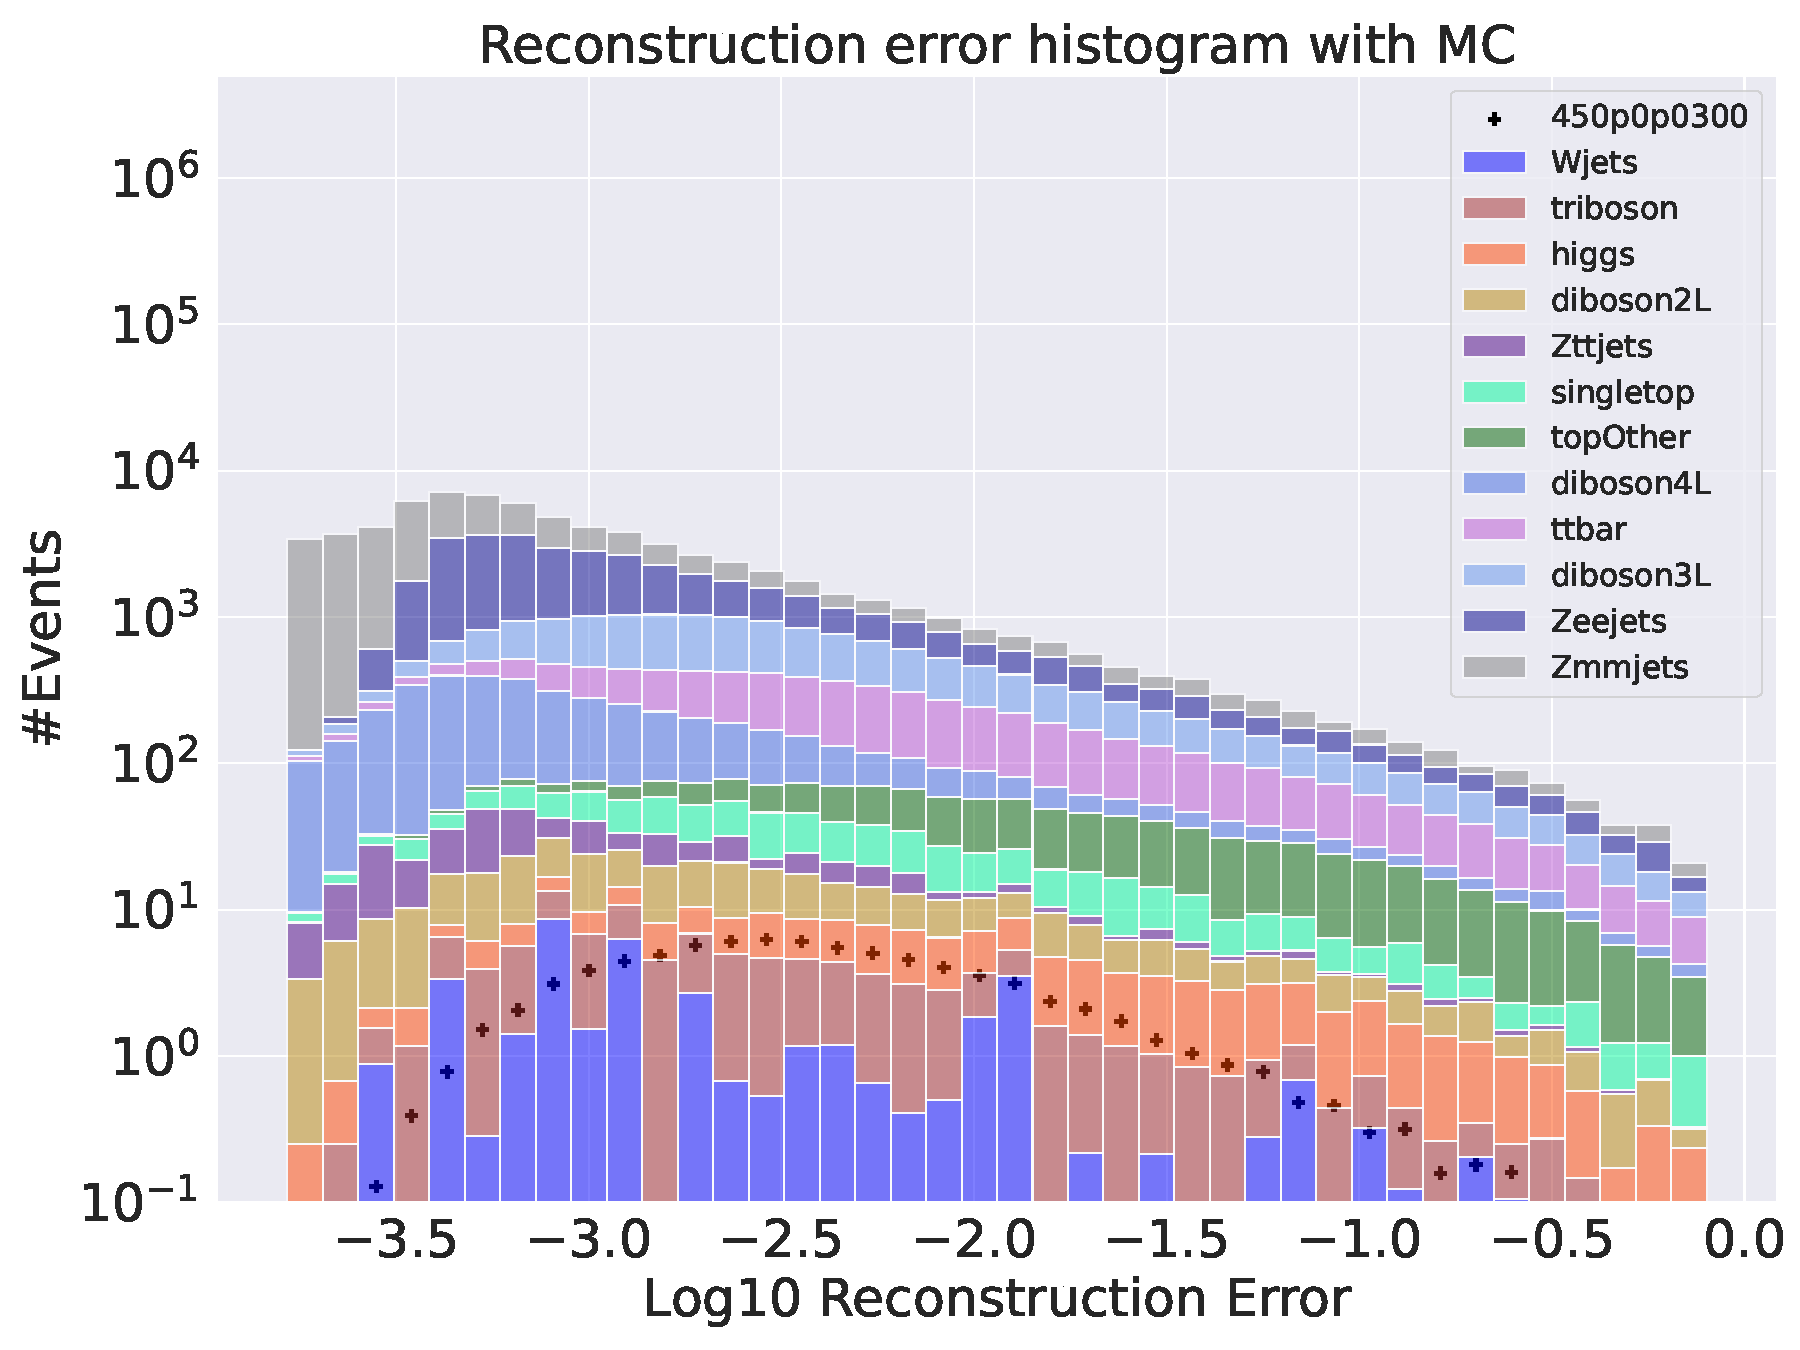
\includegraphics[width=\textwidth]{Figures/AE_testing/big/3lep/b_data_recon_big_rm3_feats_sig_450p0p0300.pdf}
        \caption{ }
        \label{fig:AE_3lep_big_450_2}
    \end{subfigure}
    \hfill
    \begin{subfigure}{.40\textwidth}
        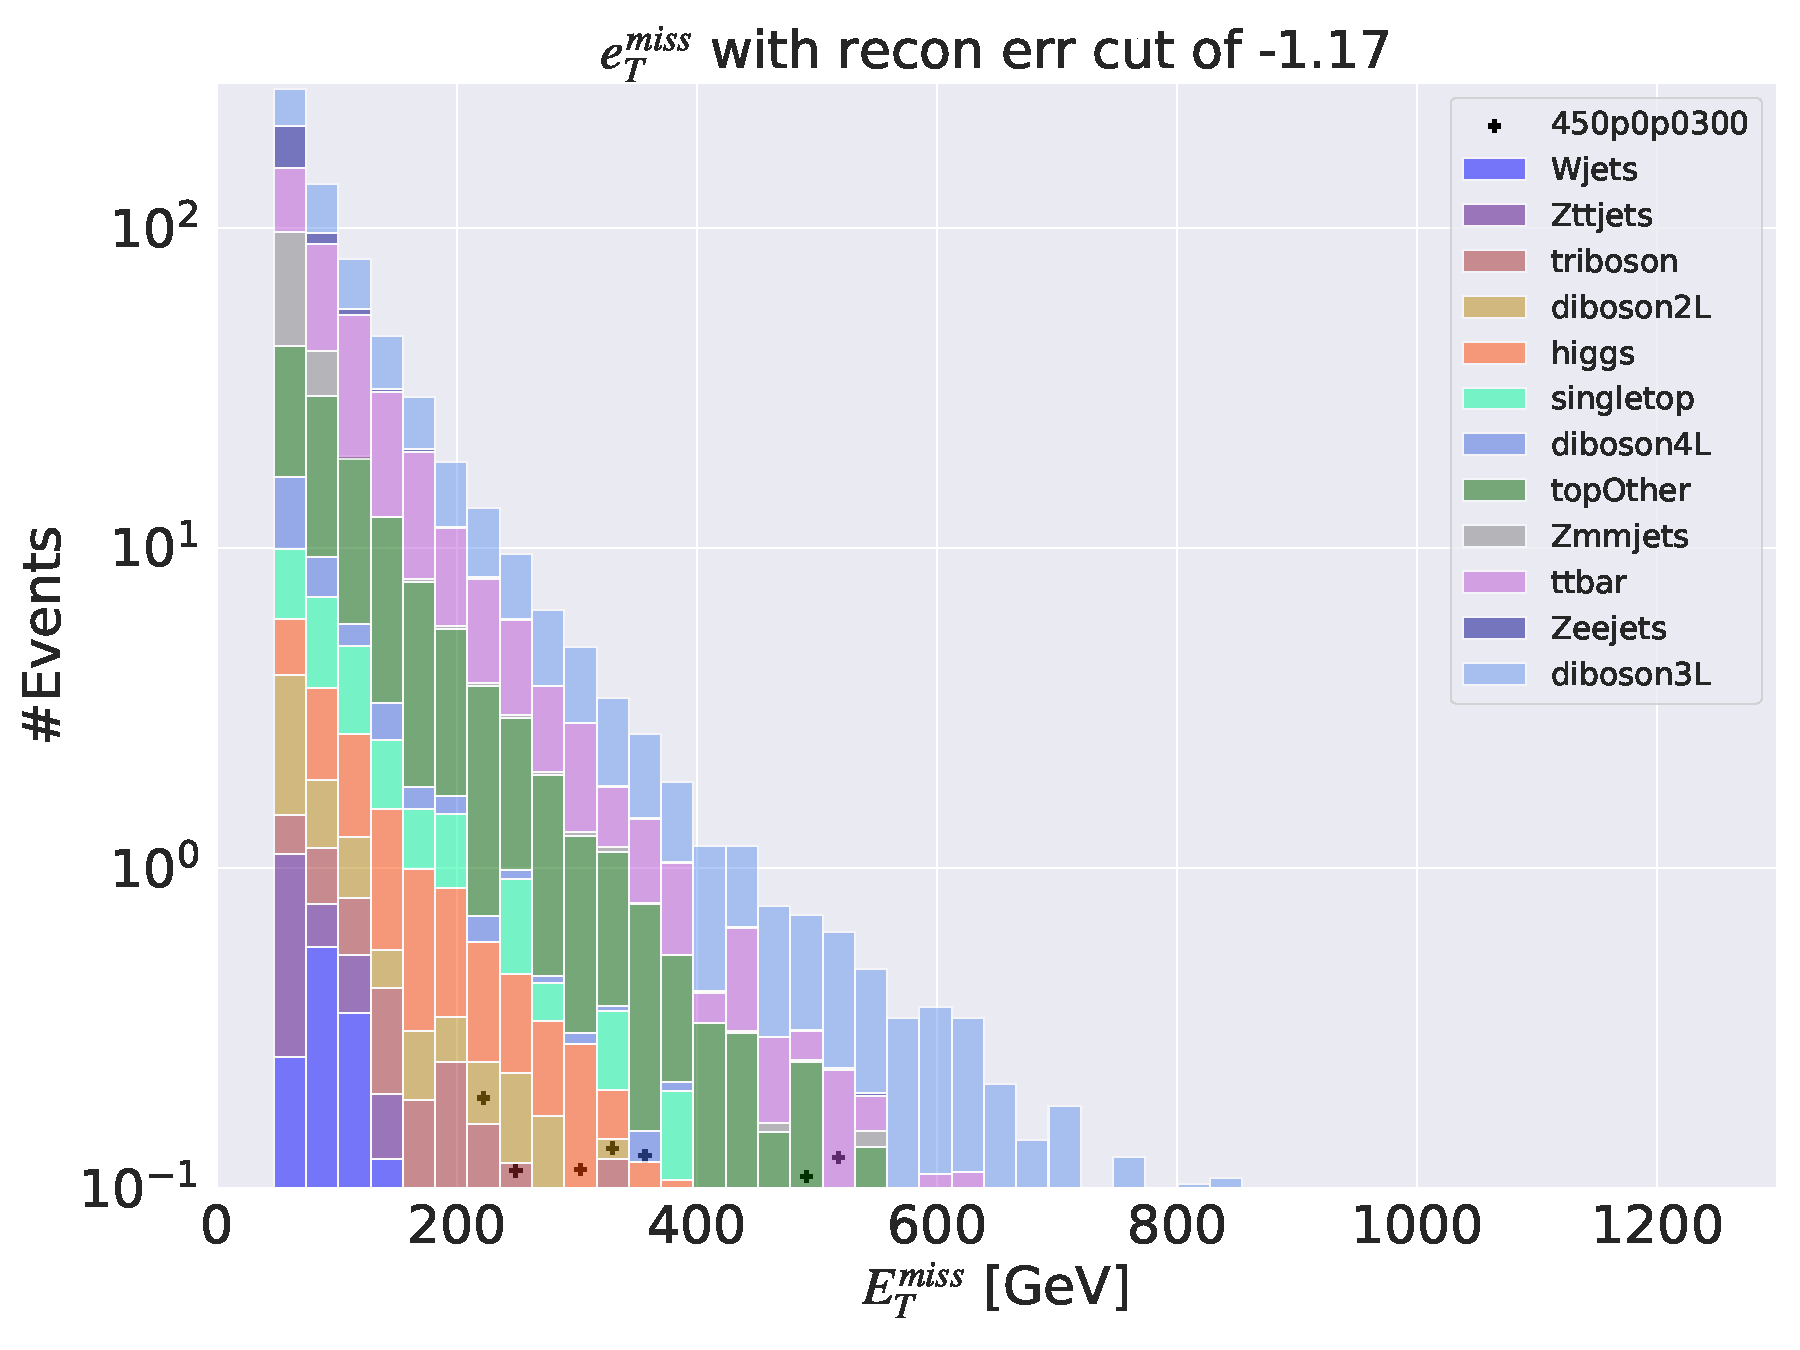
\includegraphics[width=\textwidth]{Figures/AE_testing/big/3lep/b_data_recon_big_rm3_feats_sig_450p0p0300_etmiss_recon_errcut_-1.17.pdf}
        \caption{}
        \label{fig:AE_3lep_big_etmiss_450_2}
    \end{subfigure}
    \hfill
    \begin{subfigure}{.40\textwidth}
        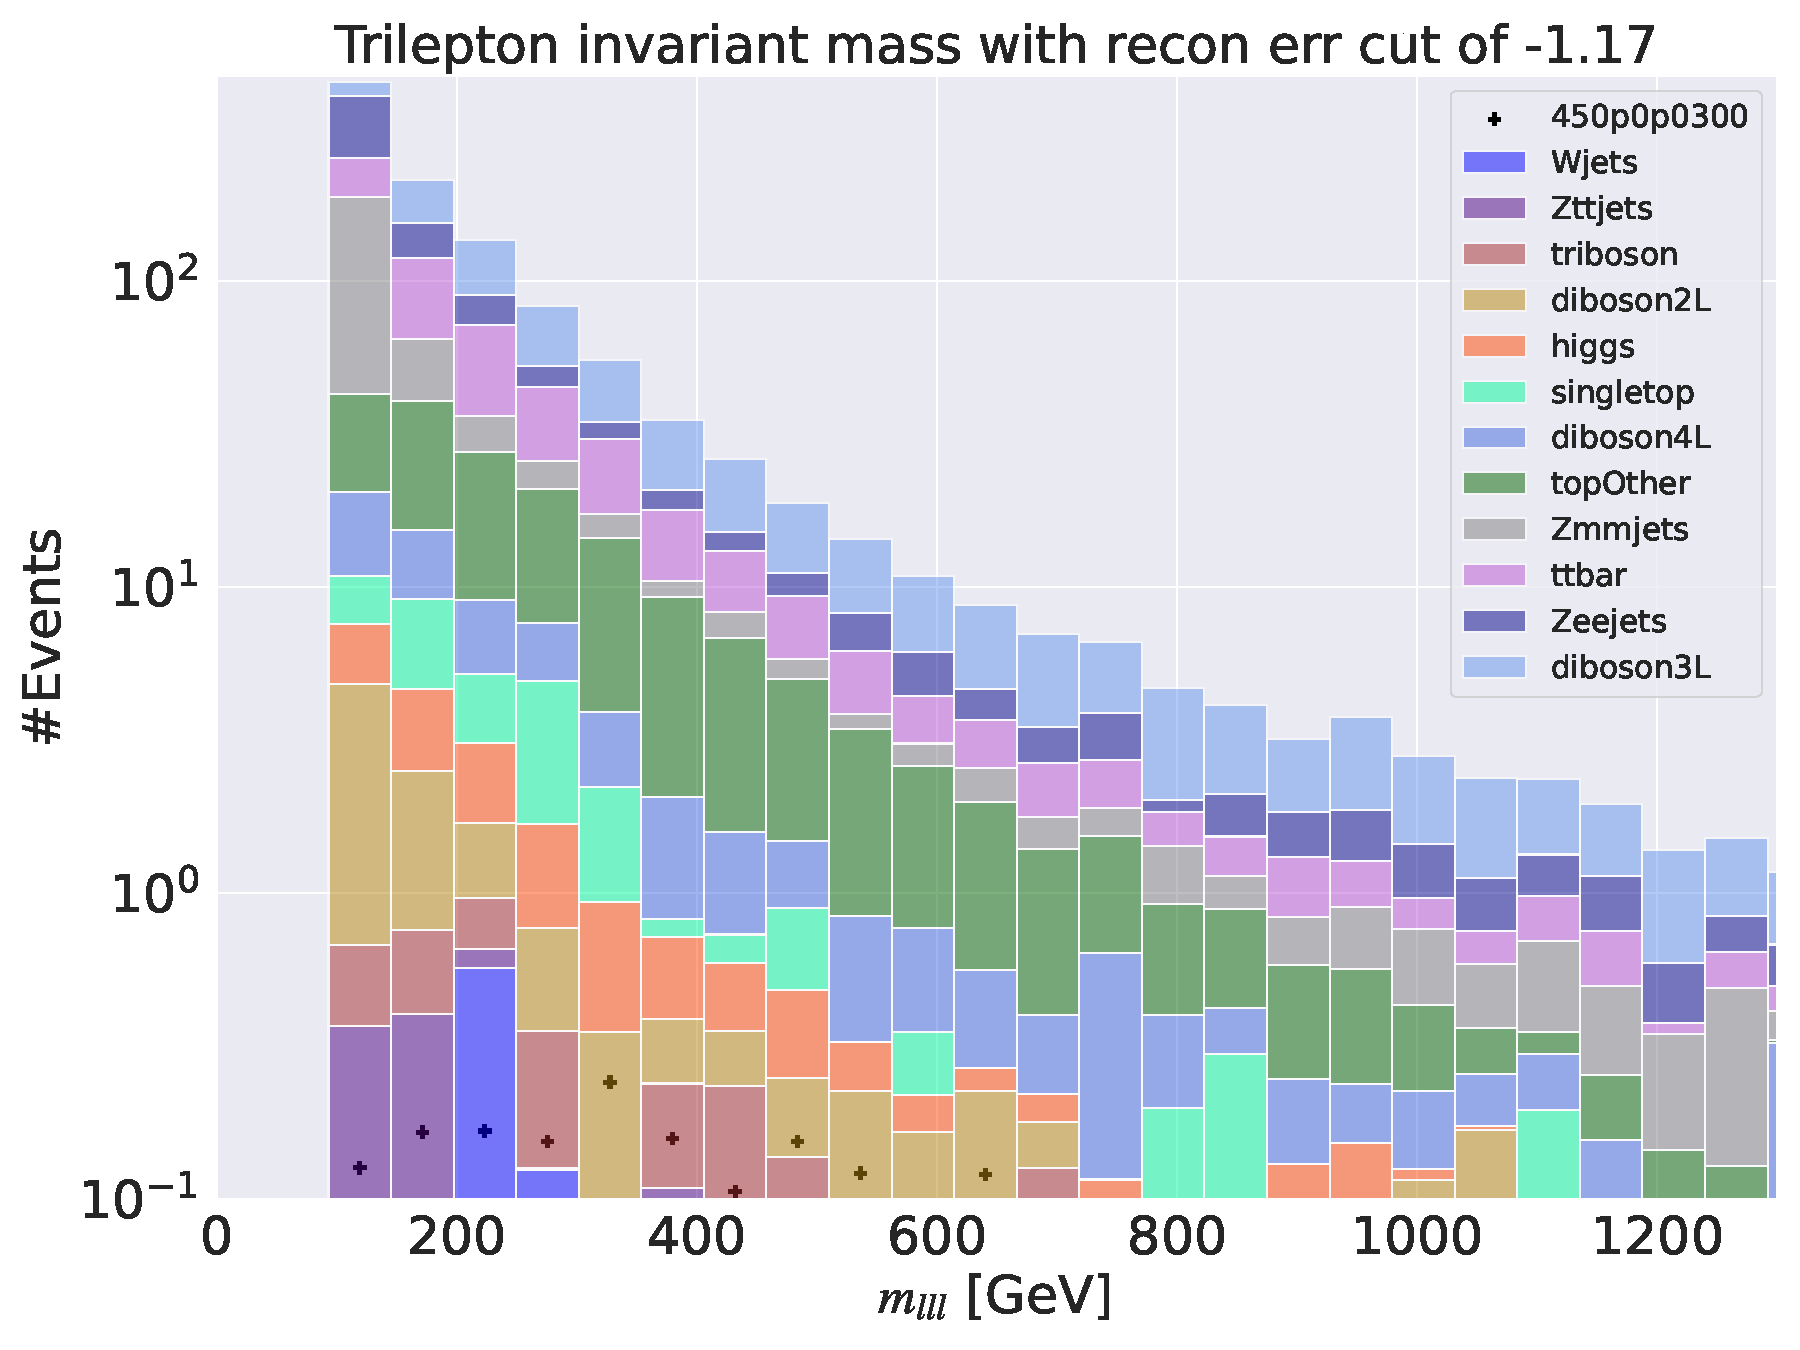
\includegraphics[width=\textwidth]{Figures/AE_testing/big/3lep/b_data_recon_big_rm3_feats_sig_450p0p0300_mlll_recon_errcut_-1.17.pdf}
        \caption{}
        \label{fig:AE_3lep_big_mlll_450_2}
    \end{subfigure}
    \hfill   
    \begin{subfigure}{.40\textwidth}
        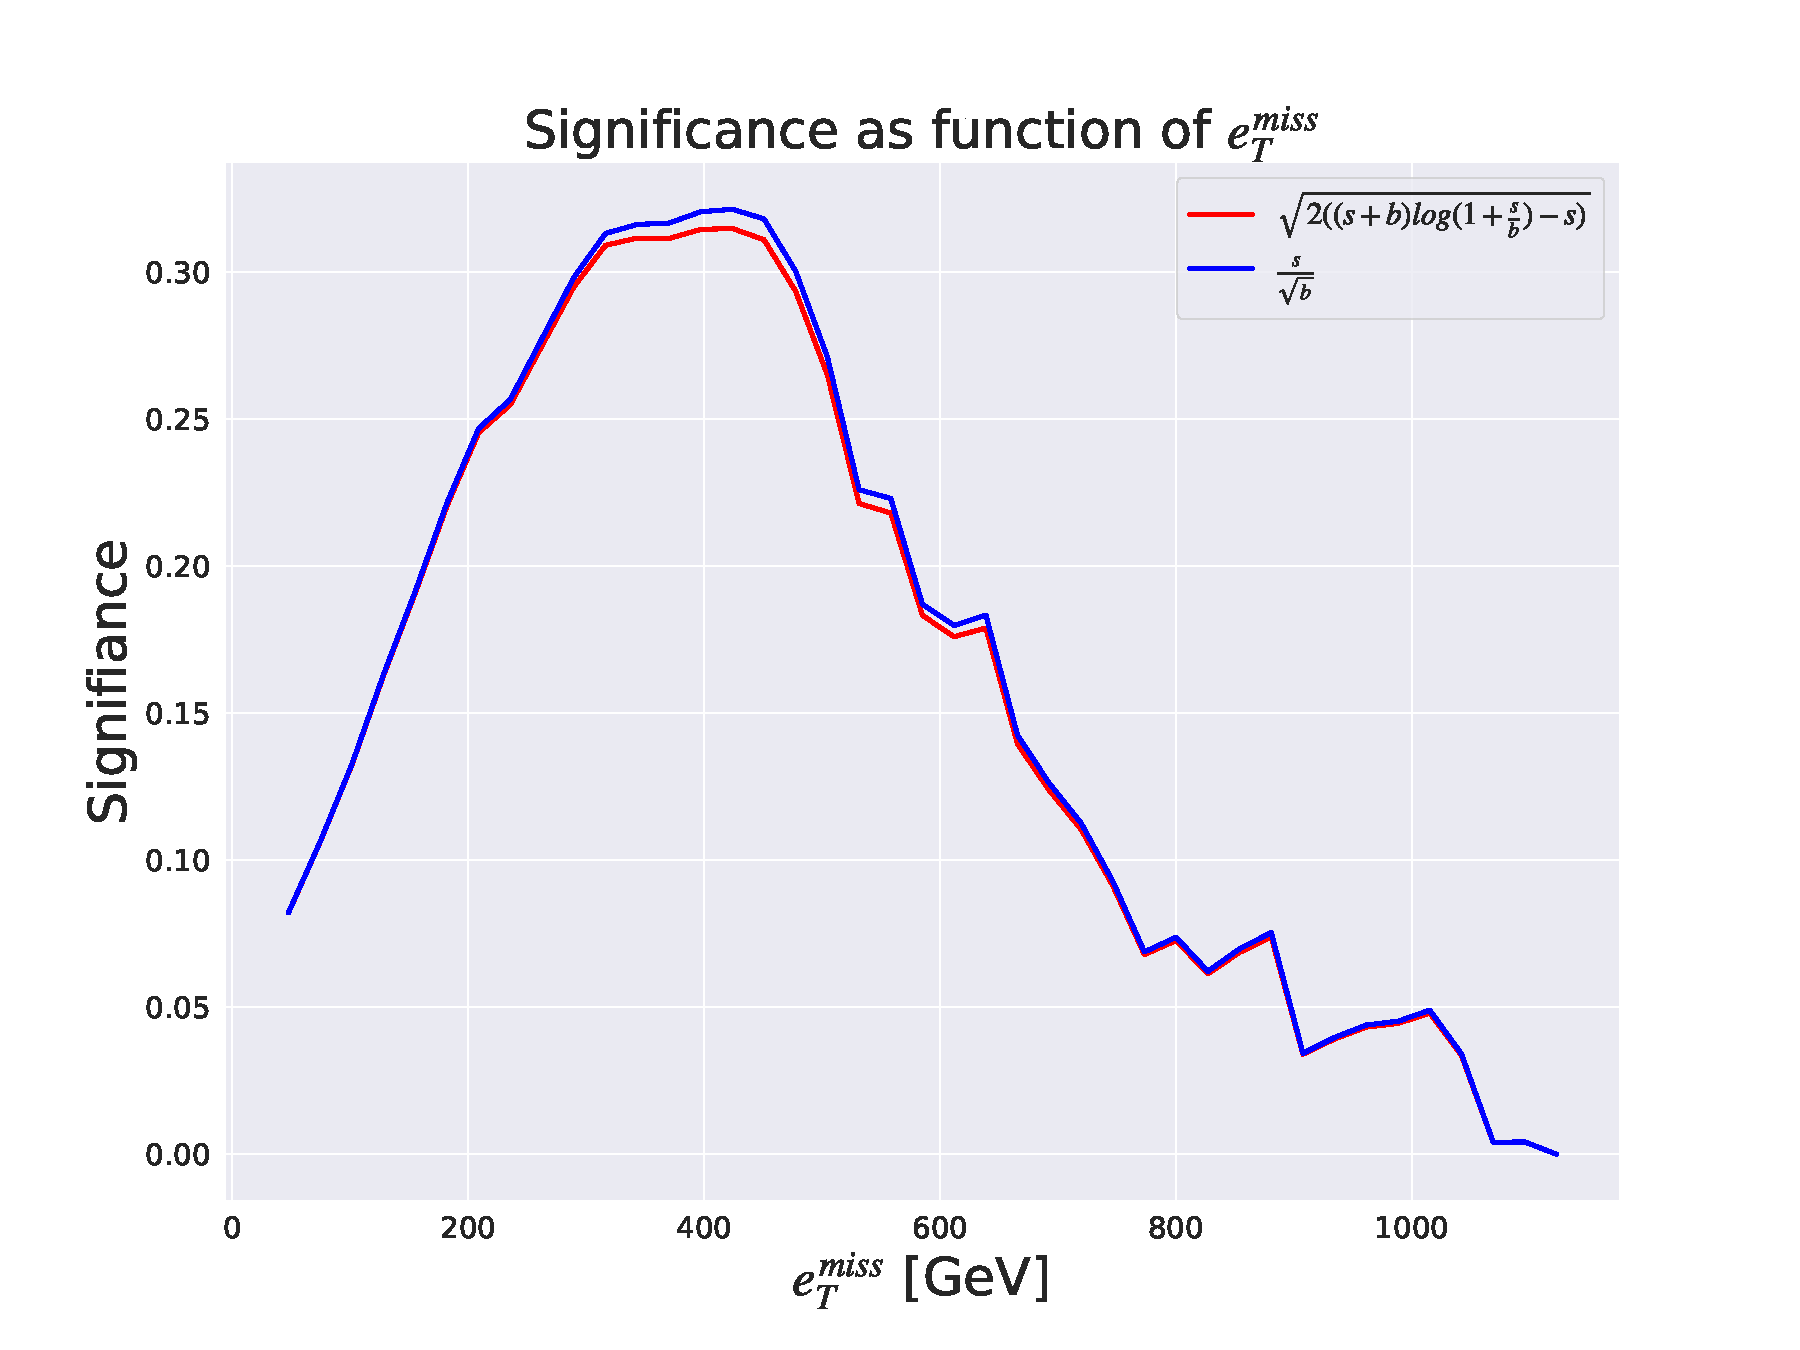
\includegraphics[width=\textwidth]{Figures/AE_testing/big/3lep/significance_etmiss_450p0p0300_-1.1736206563802147.pdf}
        \caption{}
        \label{fig:AE_3lep_big_signi_450_2}
    \end{subfigure}
    \hfill      
    \caption[3lep deep network | $450p300$ | AE | 2]{Reconstruction error, $e_T^{miss}$ signal region, $m_{lll}$ signal region and significance as function of 
    $e_T^{miss}$ for the deep regular autoencoder using the SUSY $450p300$. 
    Figure \ref{fig:AE_3lep_big_450_2} shows the reconstruction error 
    distribution for the SM MC and the SUSY signal. Here the autoencoder produce the same reconstruction error shape for both background and 
    signal. Figure \ref{fig:AE_3lep_big_etmiss_450_2} shows the $e_T^{miss}$ distribution for the SM MC and the SUSY signal in the signal region. 
    The signal region is made using a cut around $10^{-1.17}$. Most of the background is removed, with almost no signal in the signal region.
    Figure \ref{fig:AE_3lep_big_mlll_450_2} shows the $m_{lll}$ distribution for the SM MC and the SUSY signal. 
    There is almost no signal in the signal region. Figure \ref{fig:AE_3lep_big_signi_450_2} shows the significance as function of
    $e_T^{miss}$. The peak is put around a cut of about 430 GeV in the $e_T^{miss}$, with a significance of around $0.35$.}
    \label{fig:AE_3lep_big_rec_sig_signi_450_2}
\end{figure}

\begin{figure}[H]
    \centering
    \begin{subfigure}{.40\textwidth}
        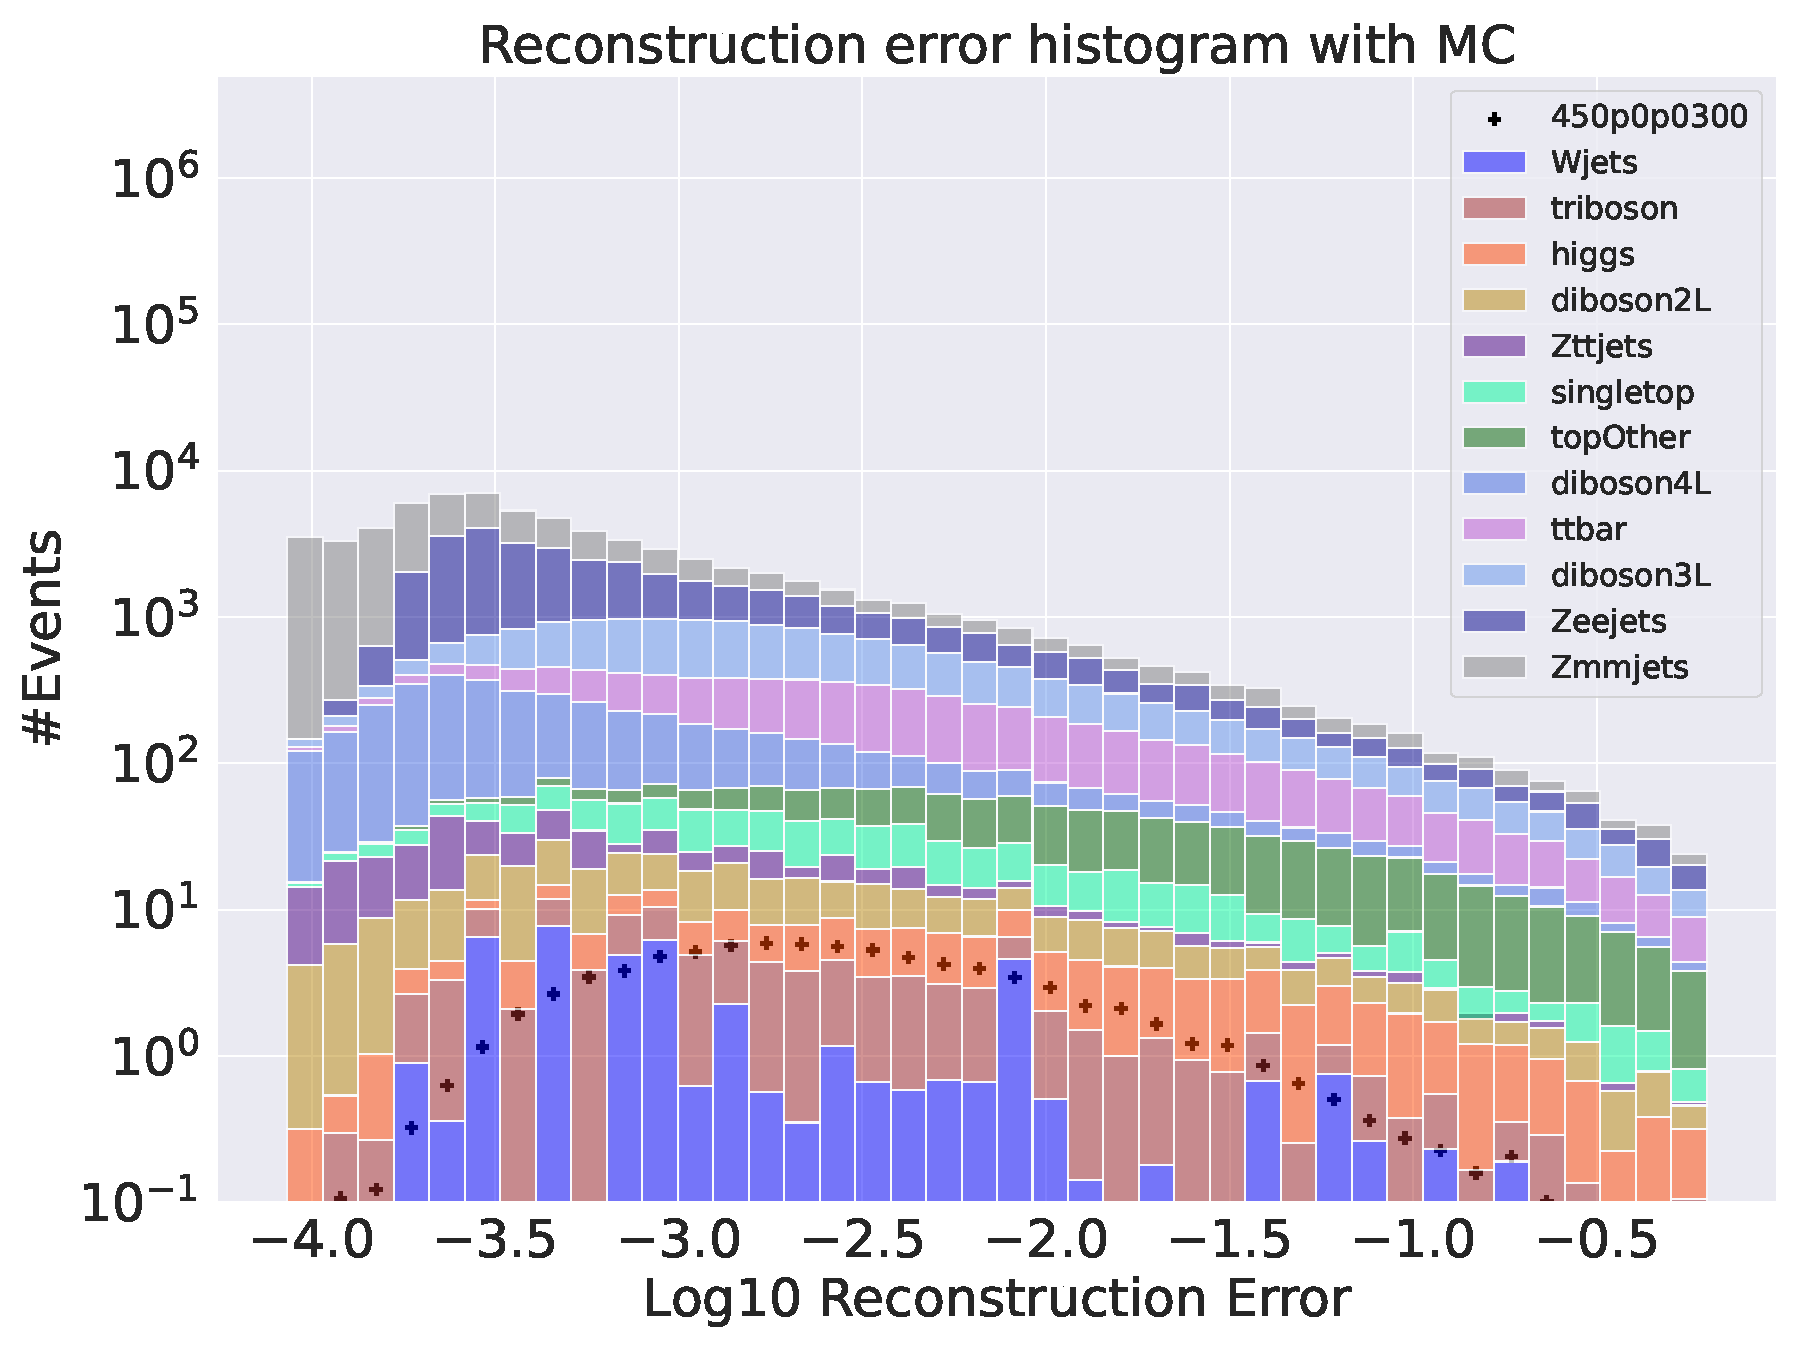
\includegraphics[width=\textwidth]{Figures/AE_testing/small/3lep/b_data_recon_big_rm3_feats_sig_450p0p0300.pdf}
        \caption{ }
        \label{fig:AE_3lep_small_450_2}
    \end{subfigure}
    \hfill
    \begin{subfigure}{.40\textwidth}
        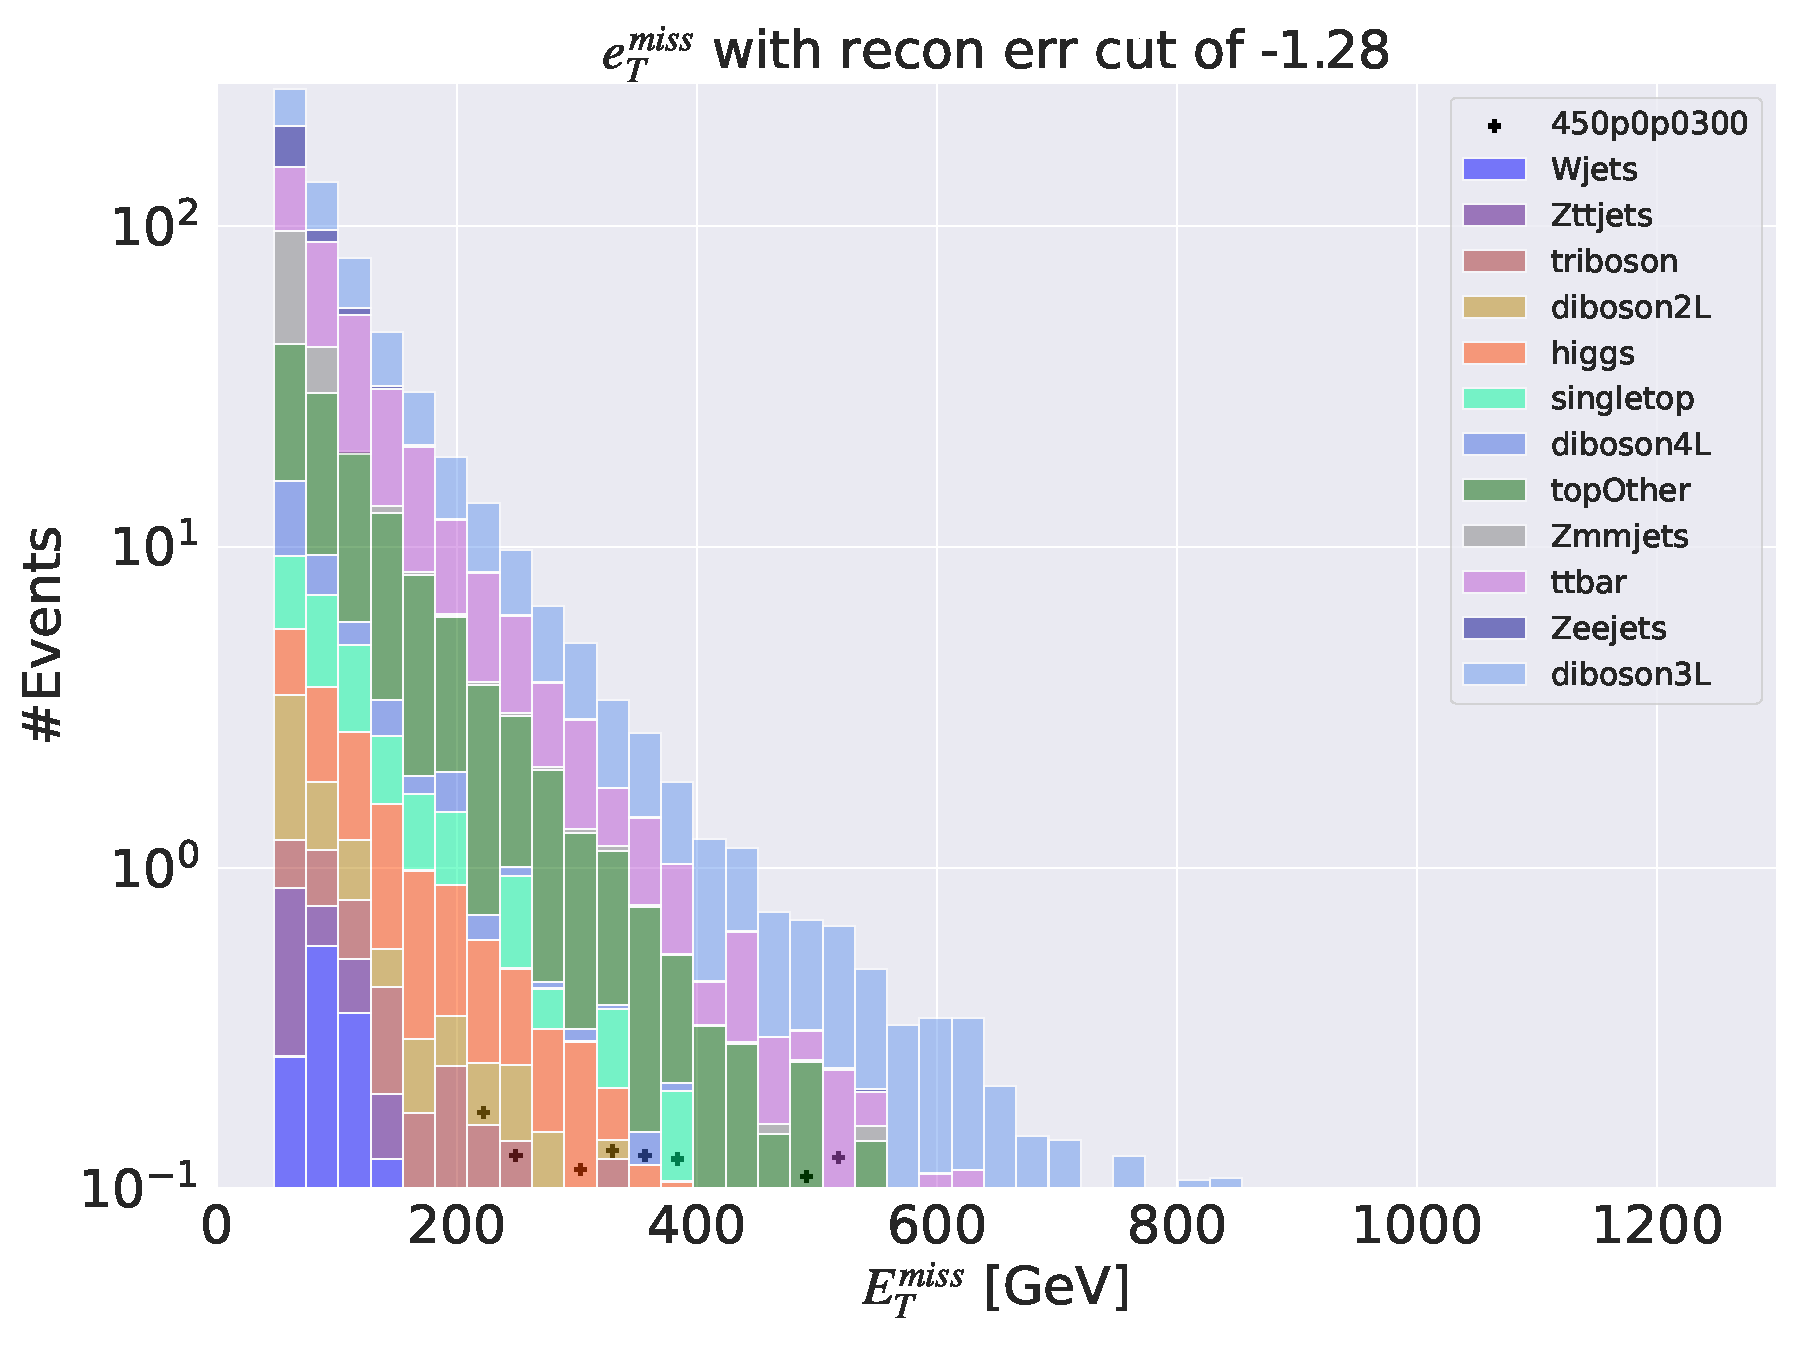
\includegraphics[width=\textwidth]{Figures/AE_testing/small/3lep/b_data_recon_big_rm3_feats_sig_450p0p0300_etmiss_recon_errcut_-1.28.pdf}
        \caption{}
        \label{fig:AE_3lep_small_etmiss_450_2}
    \end{subfigure}
    \hfill
    \begin{subfigure}{.40\textwidth}
        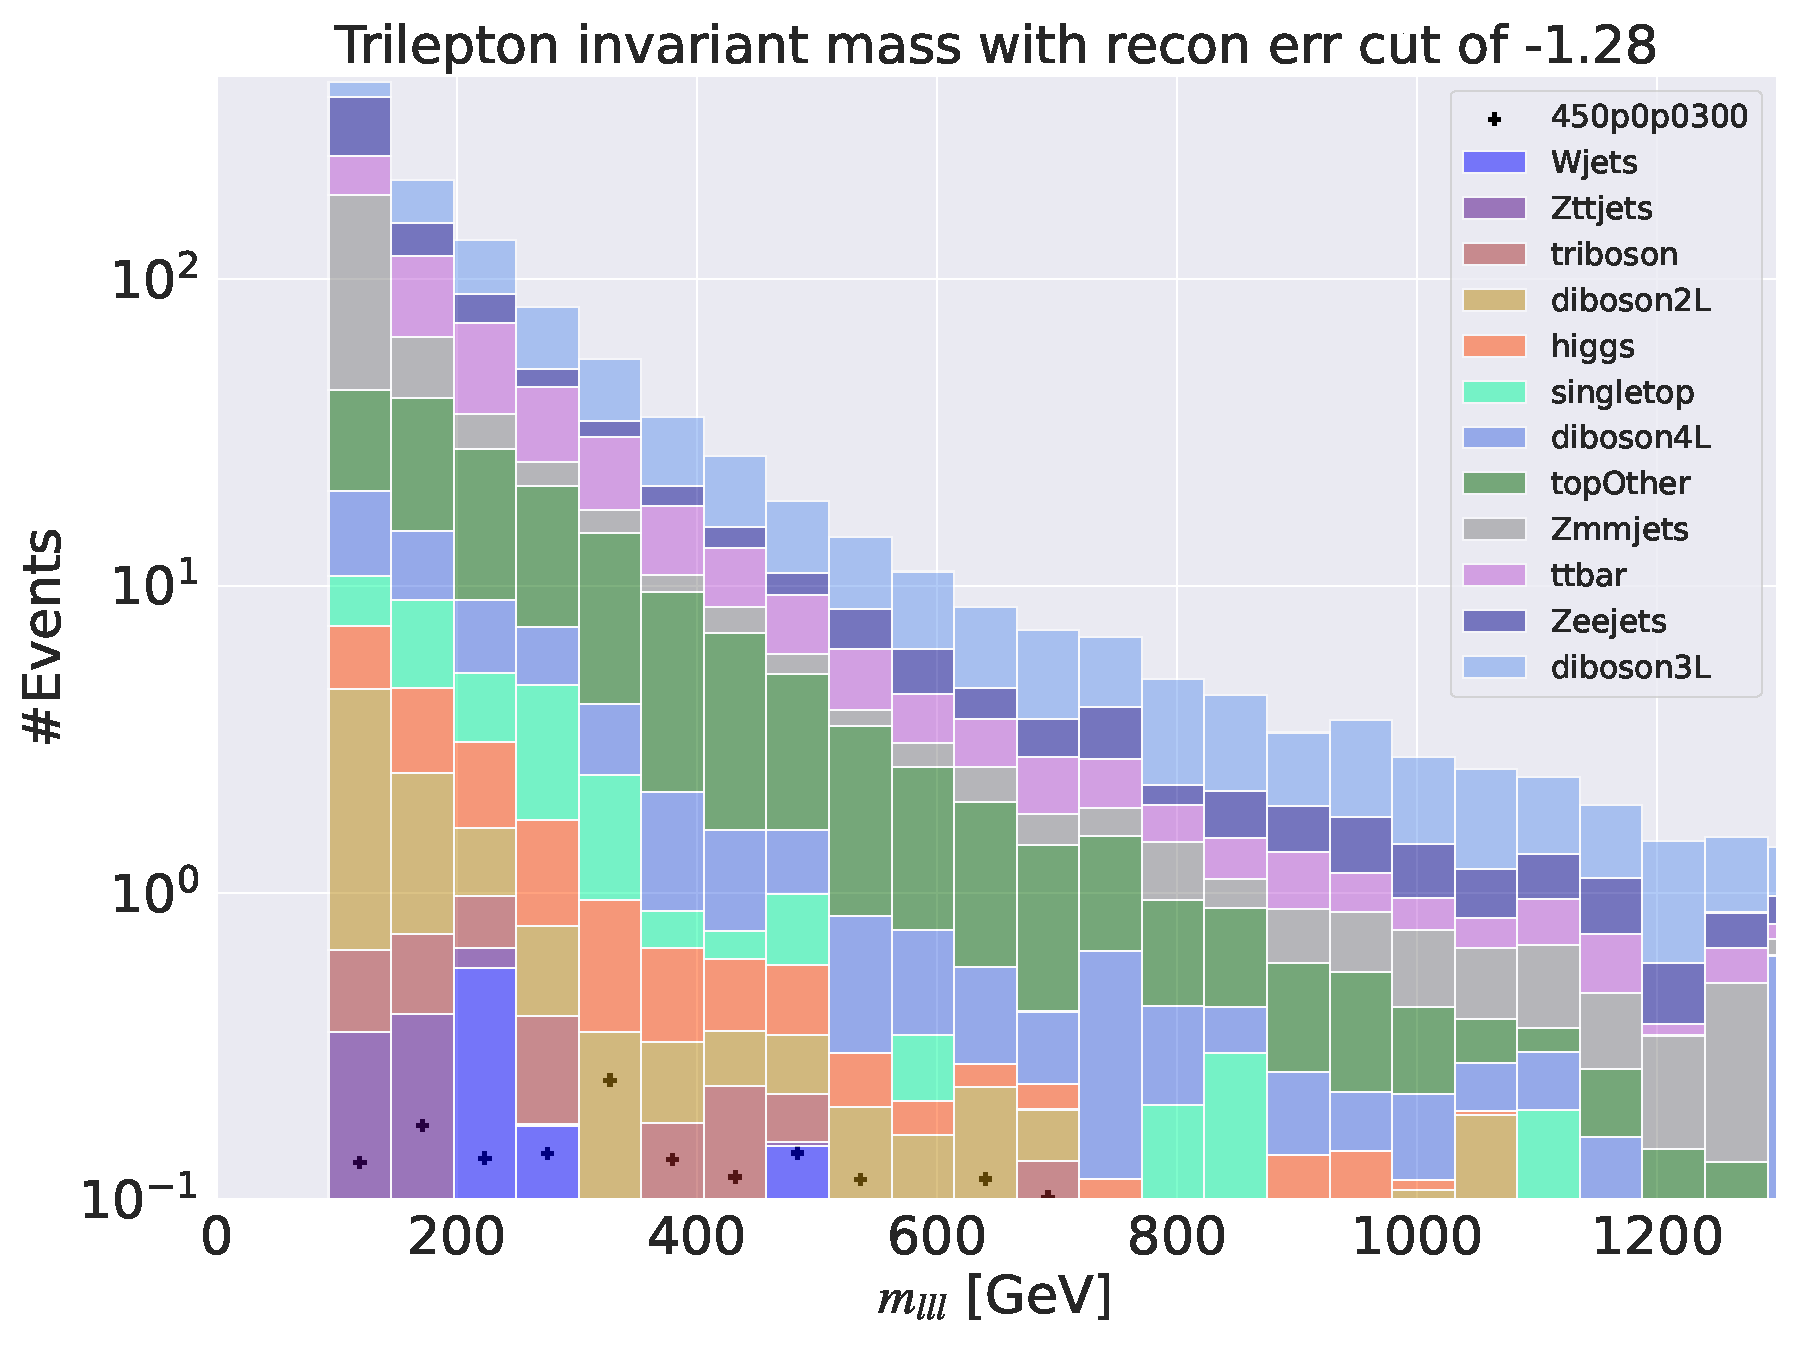
\includegraphics[width=\textwidth]{Figures/AE_testing/small/3lep/b_data_recon_big_rm3_feats_sig_450p0p0300_mlll_recon_errcut_-1.28.pdf}
        \caption{}
        \label{fig:AE_3lep_small_mlll_450_2}
    \end{subfigure}
    \hfill   
    \begin{subfigure}{.40\textwidth}
        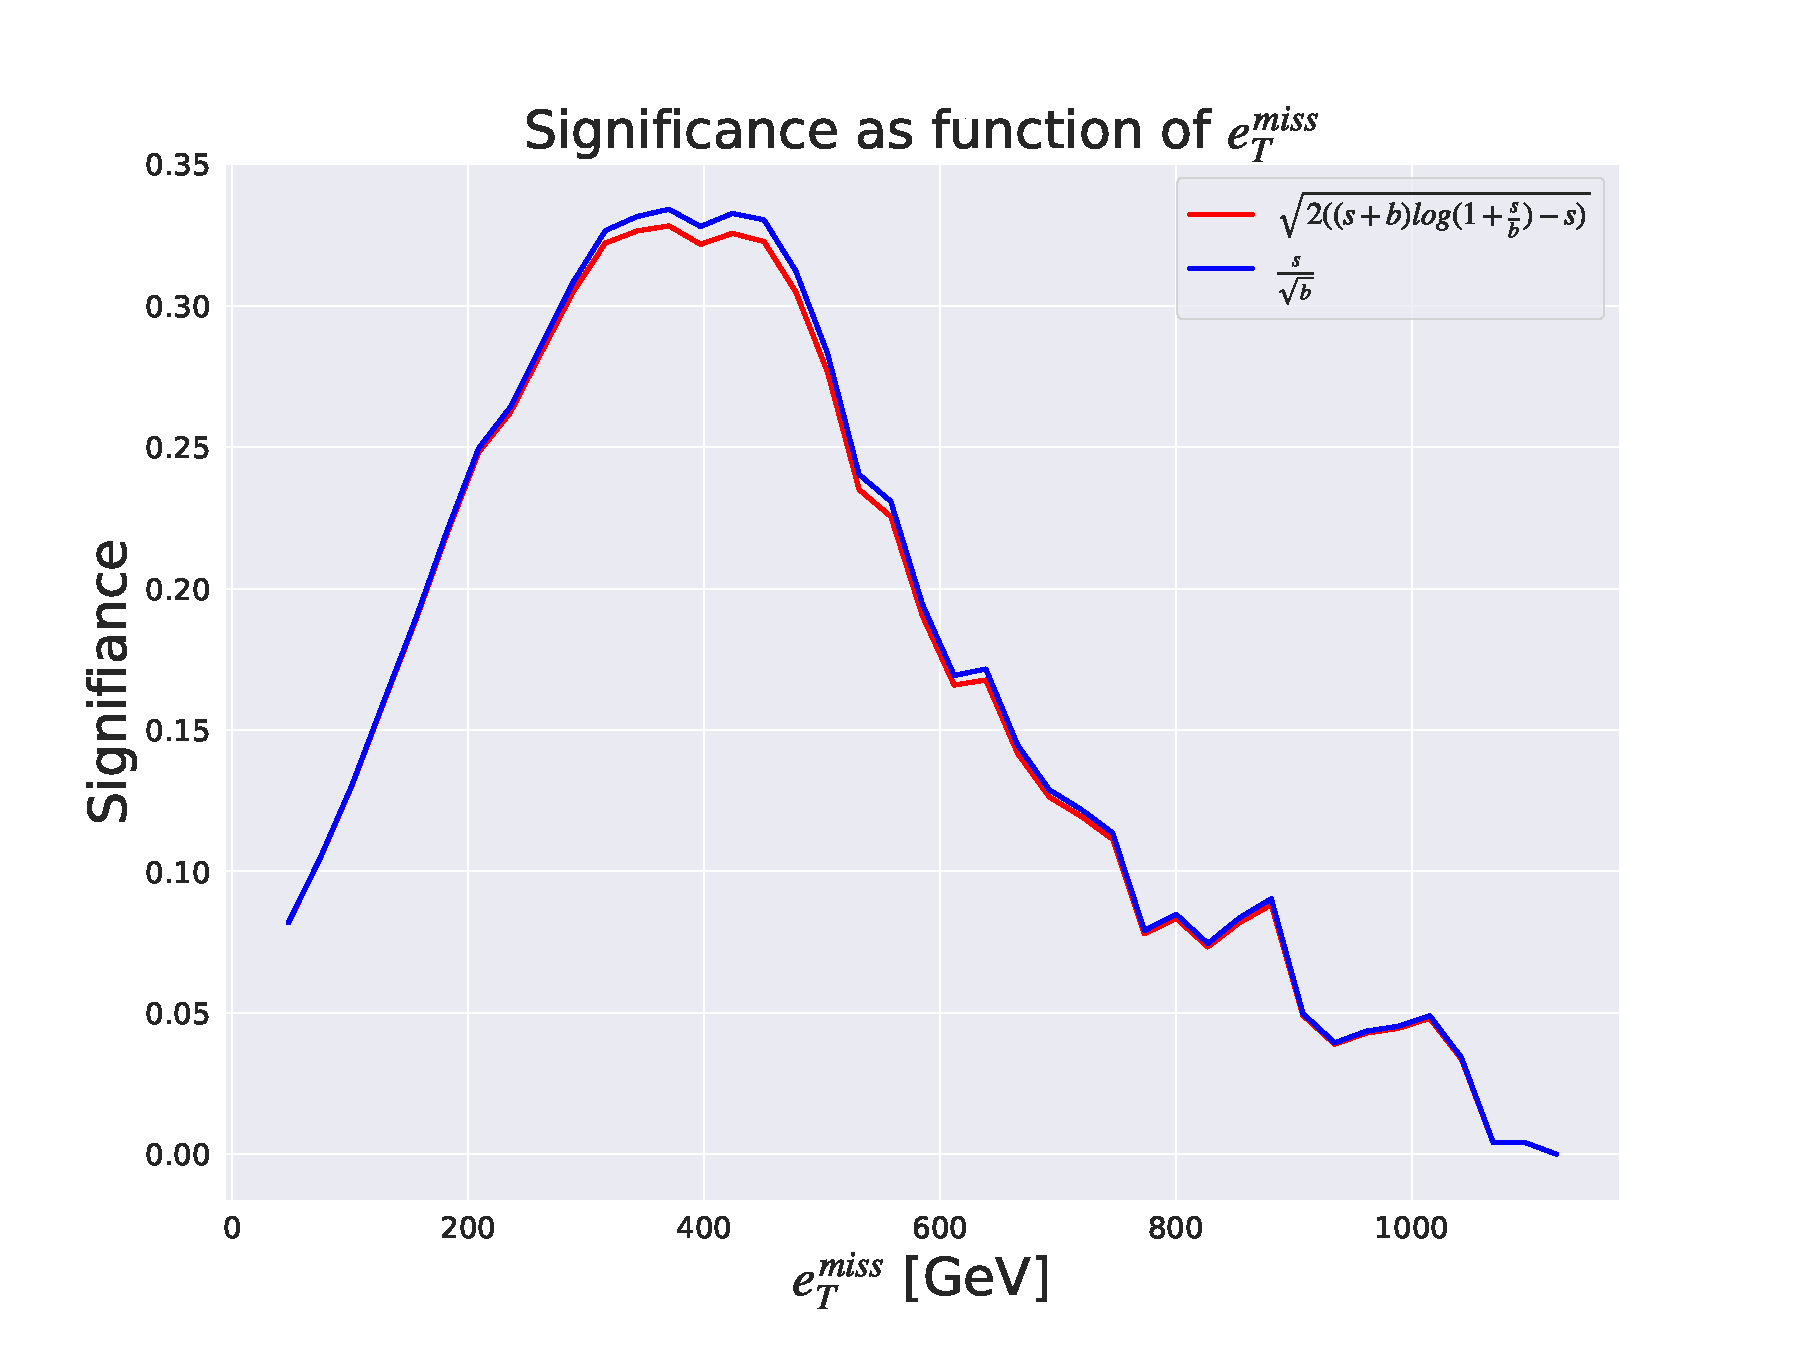
\includegraphics[width=\textwidth]{Figures/AE_testing/small/3lep/significance_etmiss_450p0p0300_-1.2800970222462997.pdf}
        \caption{}
        \label{fig:AE_3lep_small_signi_450_2}
    \end{subfigure}
    \hfill      
    \caption[3lep shallow network | $450p300$ | AE | 2]{Reconstruction error, $e_T^{miss}$ signal region, $m_{lll}$ signal region and significance as function of 
    $e_T^{miss}$ for the shallow regular autoencoder. Here the SUSY $450p300$ model is used. 
    Figure \ref{fig:AE_3lep_small_450_2} shows the reconstruction error 
    distribution for the SM MC and the SUSY signal. Here the autoencoder produce the same reconstruction error shape for both background and 
    signal. Figure \ref{fig:AE_3lep_small_etmiss_450_2} shows the $e_T^{miss}$ distribution for the SM MC and the SUSY signal in the signal region. 
    The signal region is made using a cut around $10^{-1.28}$. Most of the background is removed, with almost no signal in the signal region.
    Figure \ref{fig:AE_3lep_small_mlll_450_2} shows the $m_{lll}$ distribution for the SM MC and the SUSY signal. 
    There is almost no signal in the signal region. Figure \ref{fig:AE_3lep_small_signi_450_2} shows the significance as function of
    $e_T^{miss}$. The peak is put around a cut of about 380 GeV in the $e_T^{miss}$, with a significance of around $0.33$.}
    \label{fig:AE_3lep_small_rec_sig_signi_450_2}
\end{figure}








\begin{figure}[H]
    \centering
    \begin{subfigure}{.40\textwidth}
        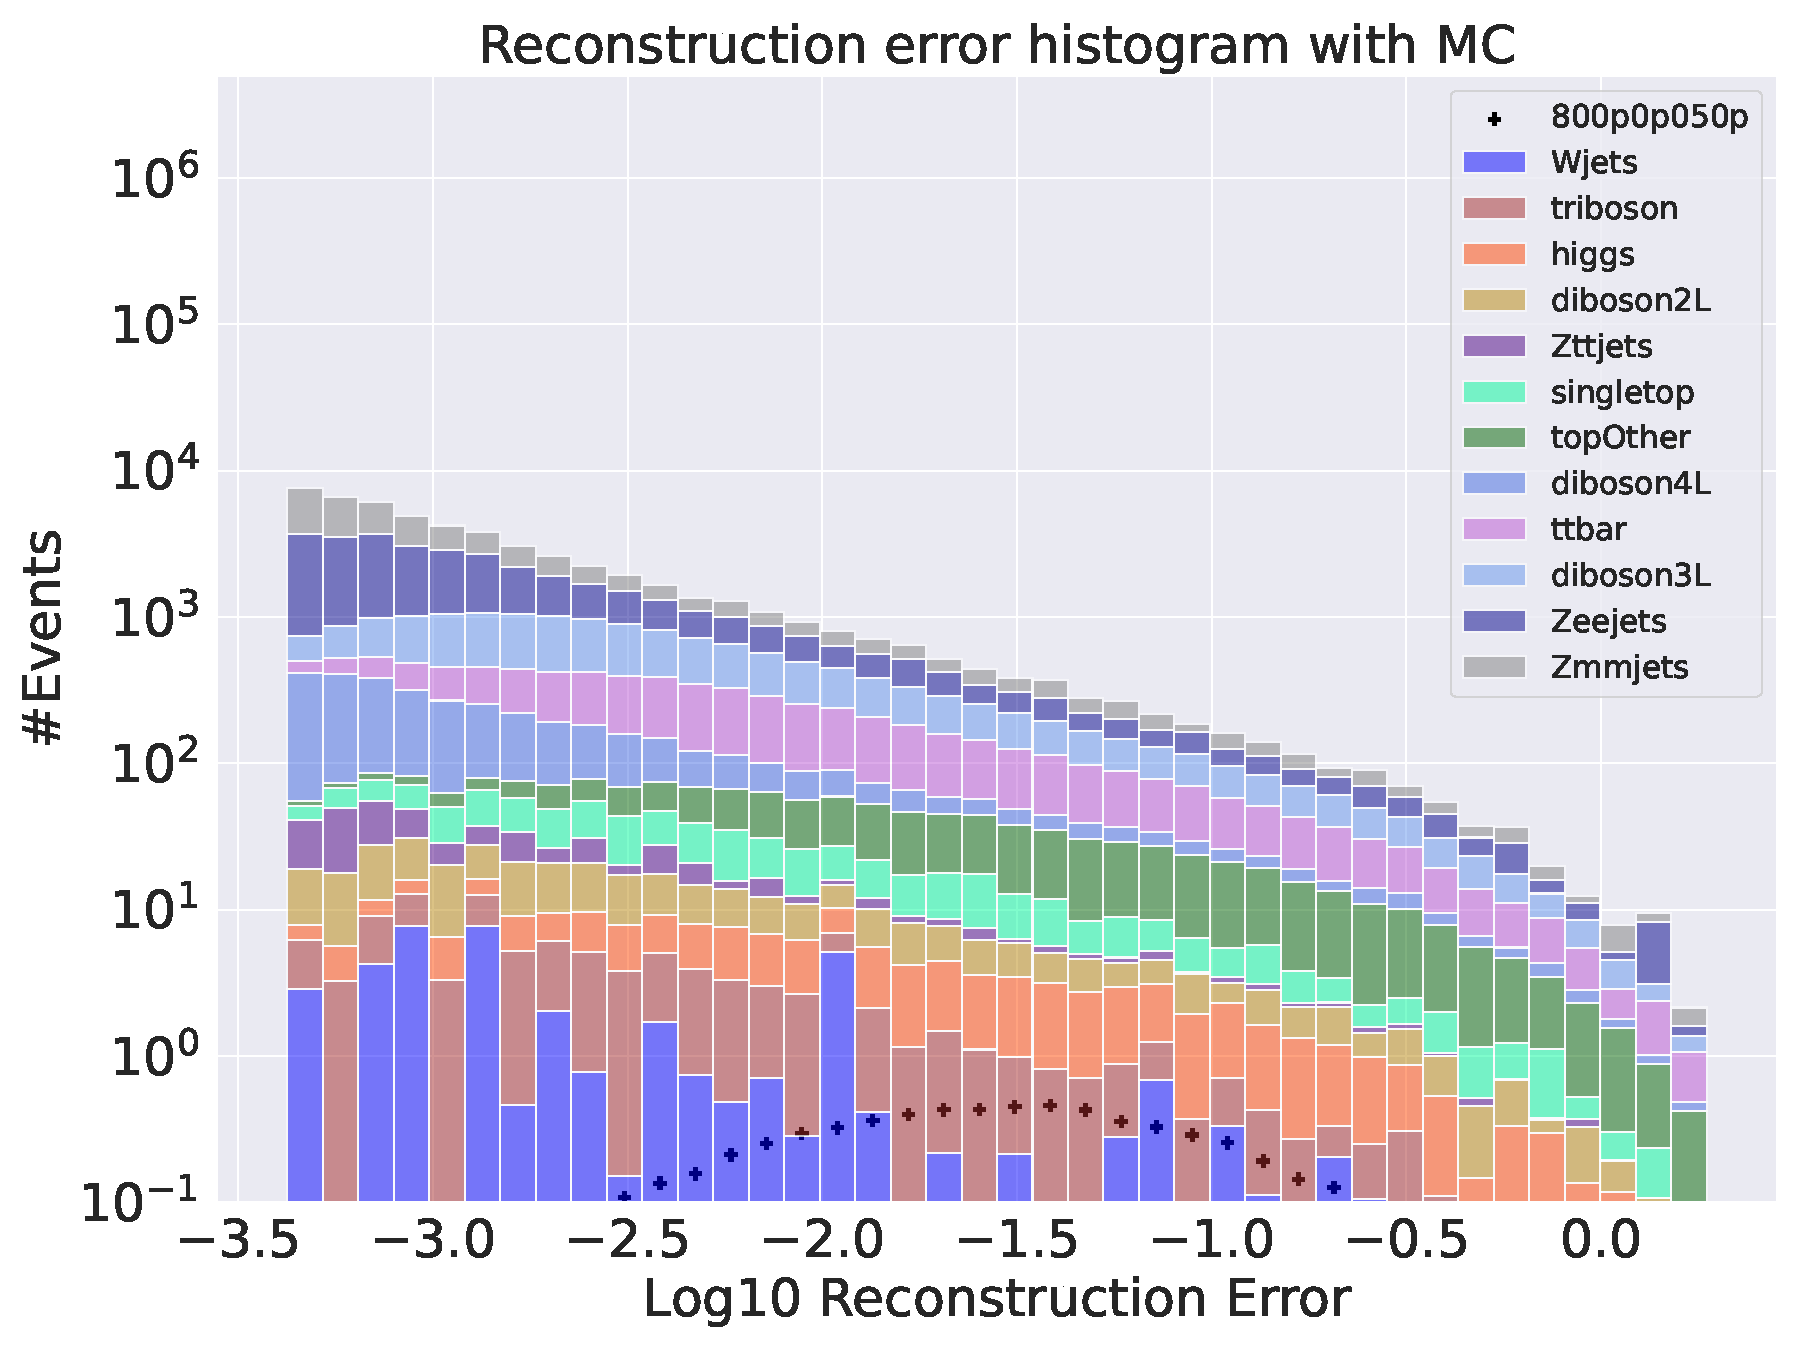
\includegraphics[width=\textwidth]{Figures/AE_testing/big/3lep/b_data_recon_big_rm3_feats_sig_800p0p050p.pdf}
        \caption{ }
        \label{fig:AE_3lep_big_800_2}
    \end{subfigure}
    \hfill
    \begin{subfigure}{.40\textwidth}
        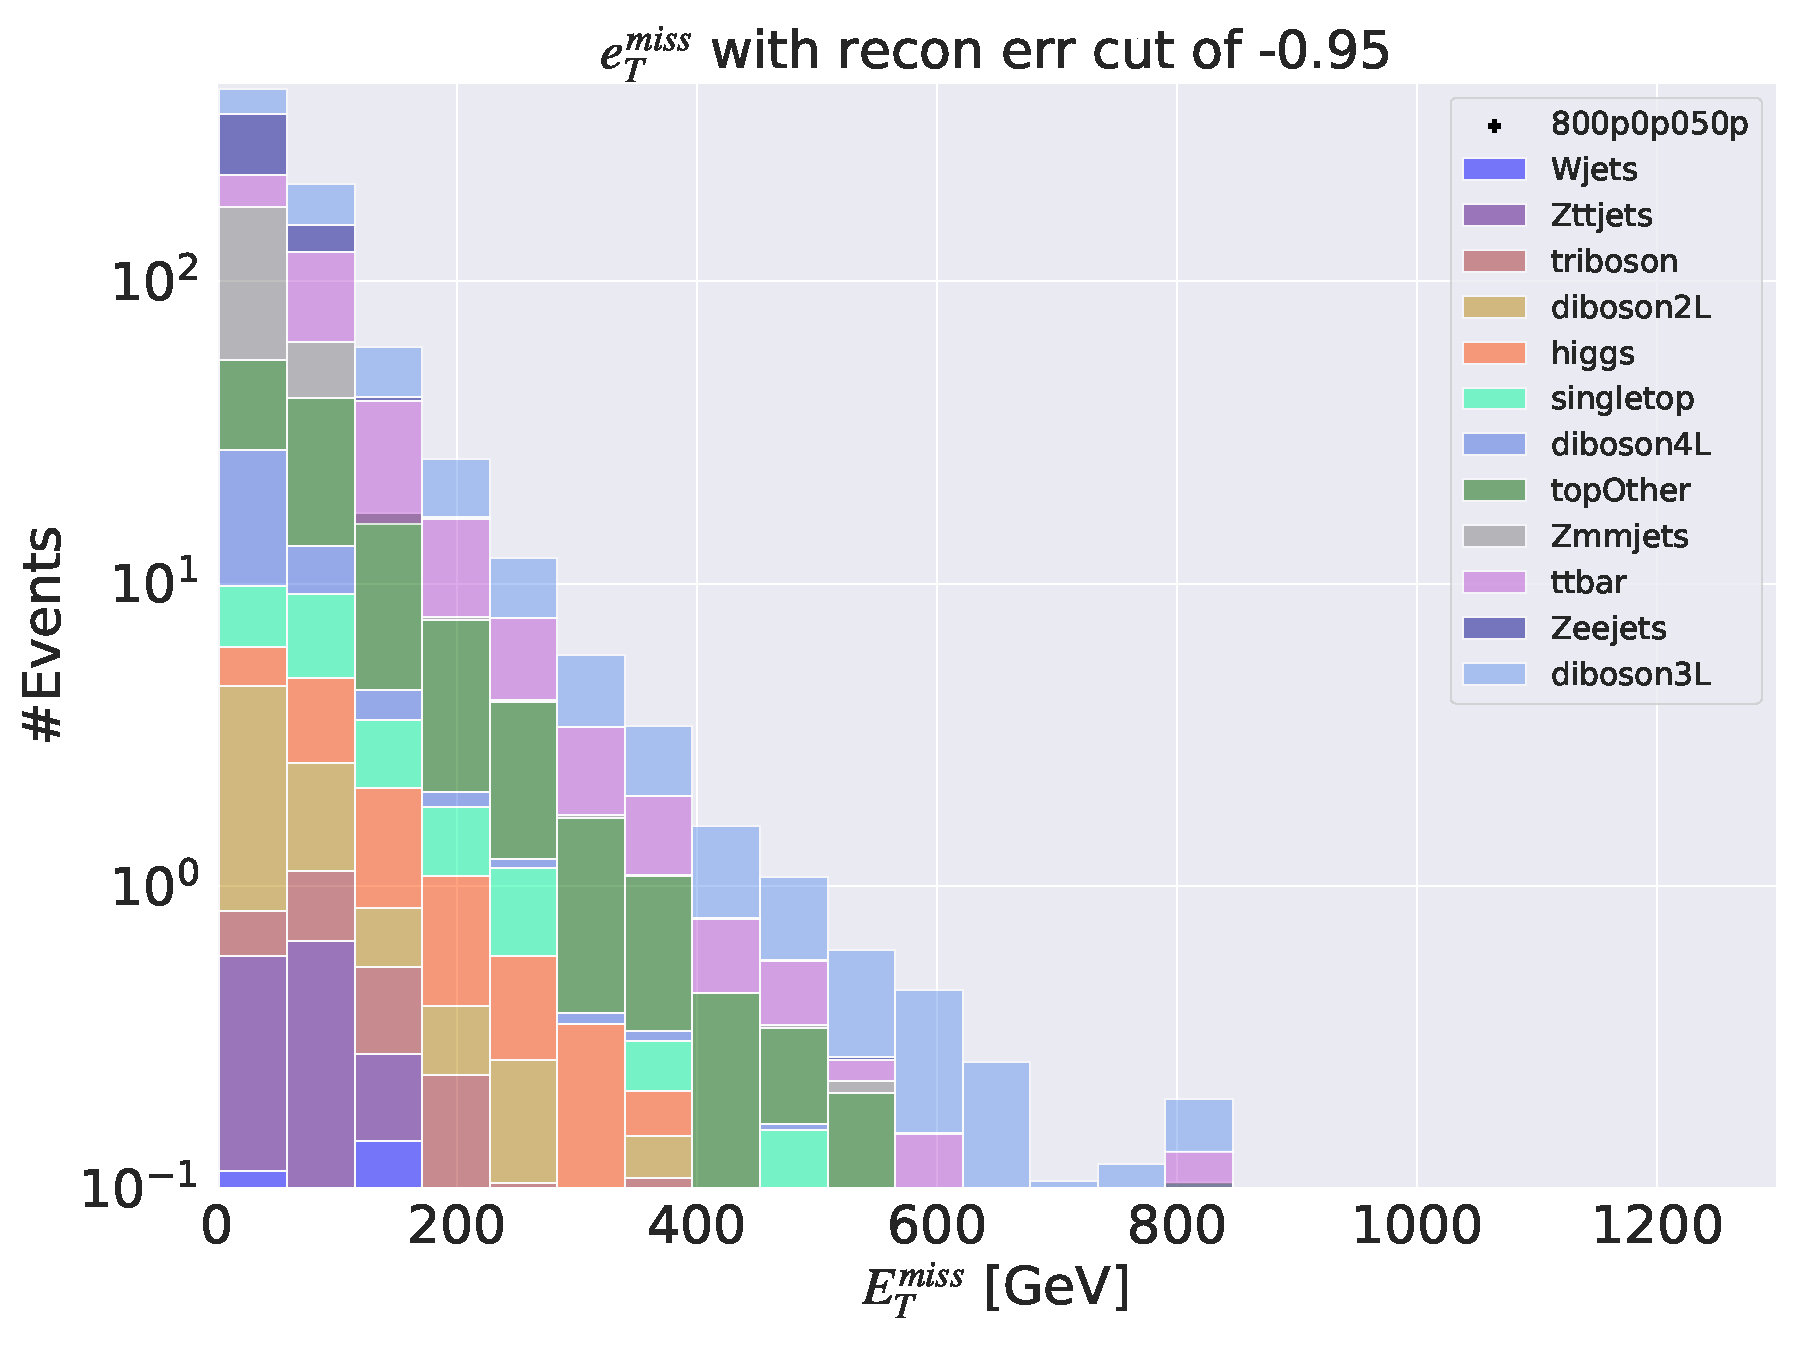
\includegraphics[width=\textwidth]{Figures/AE_testing/big/3lep/b_data_recon_big_rm3_feats_sig_800p0p050p_etmiss_recon_errcut_-0.95.pdf}
        \caption{}
        \label{fig:AE_3lep_big_etmiss_800_2}
    \end{subfigure}
    \hfill
    \begin{subfigure}{.40\textwidth}
        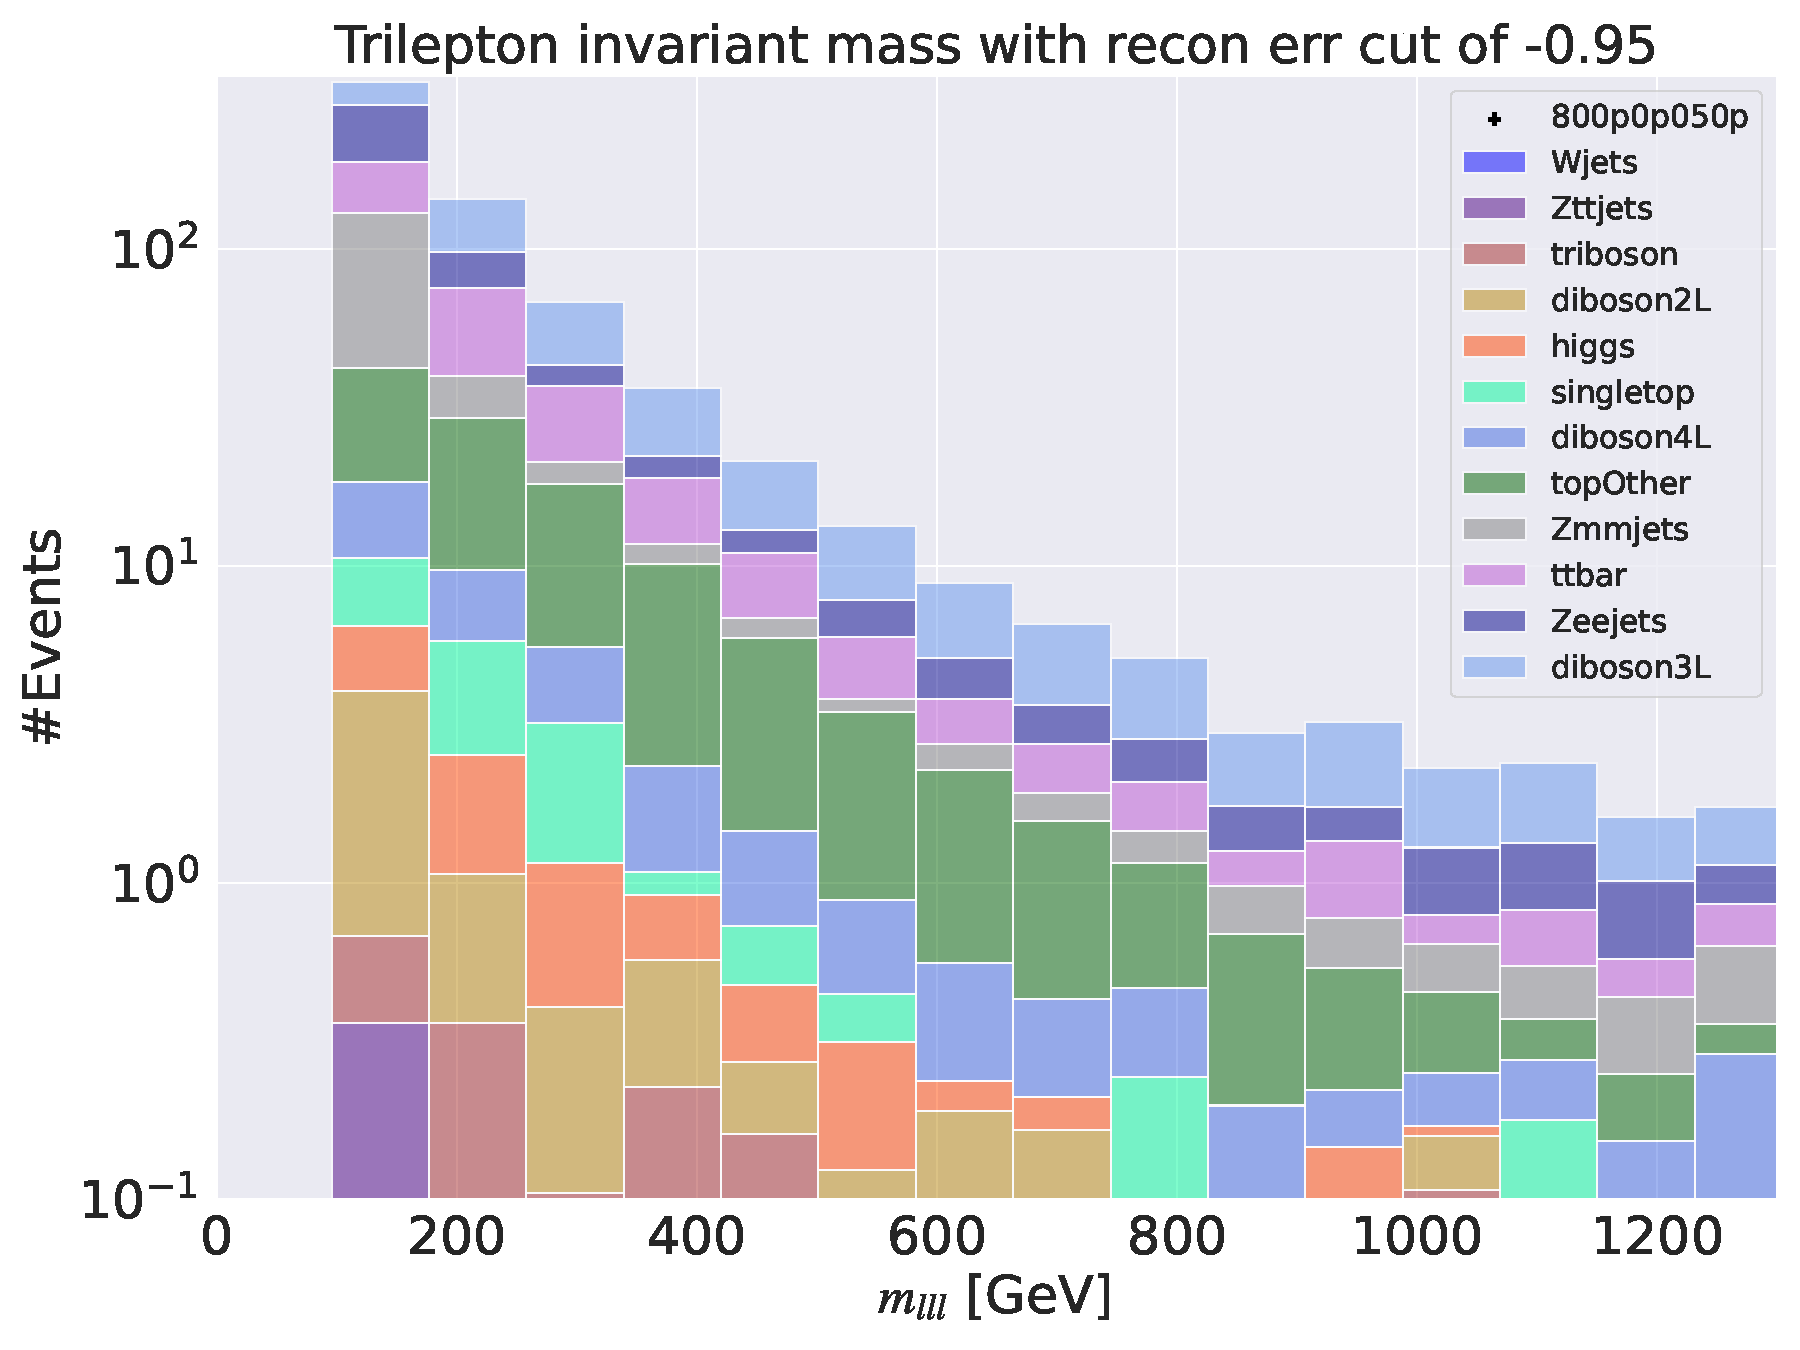
\includegraphics[width=\textwidth]{Figures/AE_testing/big/3lep/b_data_recon_big_rm3_feats_sig_800p0p050p_mlll_recon_errcut_-0.95.pdf}
        \caption{}
        \label{fig:AE_3lep_big_mlll_800_2}
    \end{subfigure}
    \hfill   
    \begin{subfigure}{.40\textwidth}
        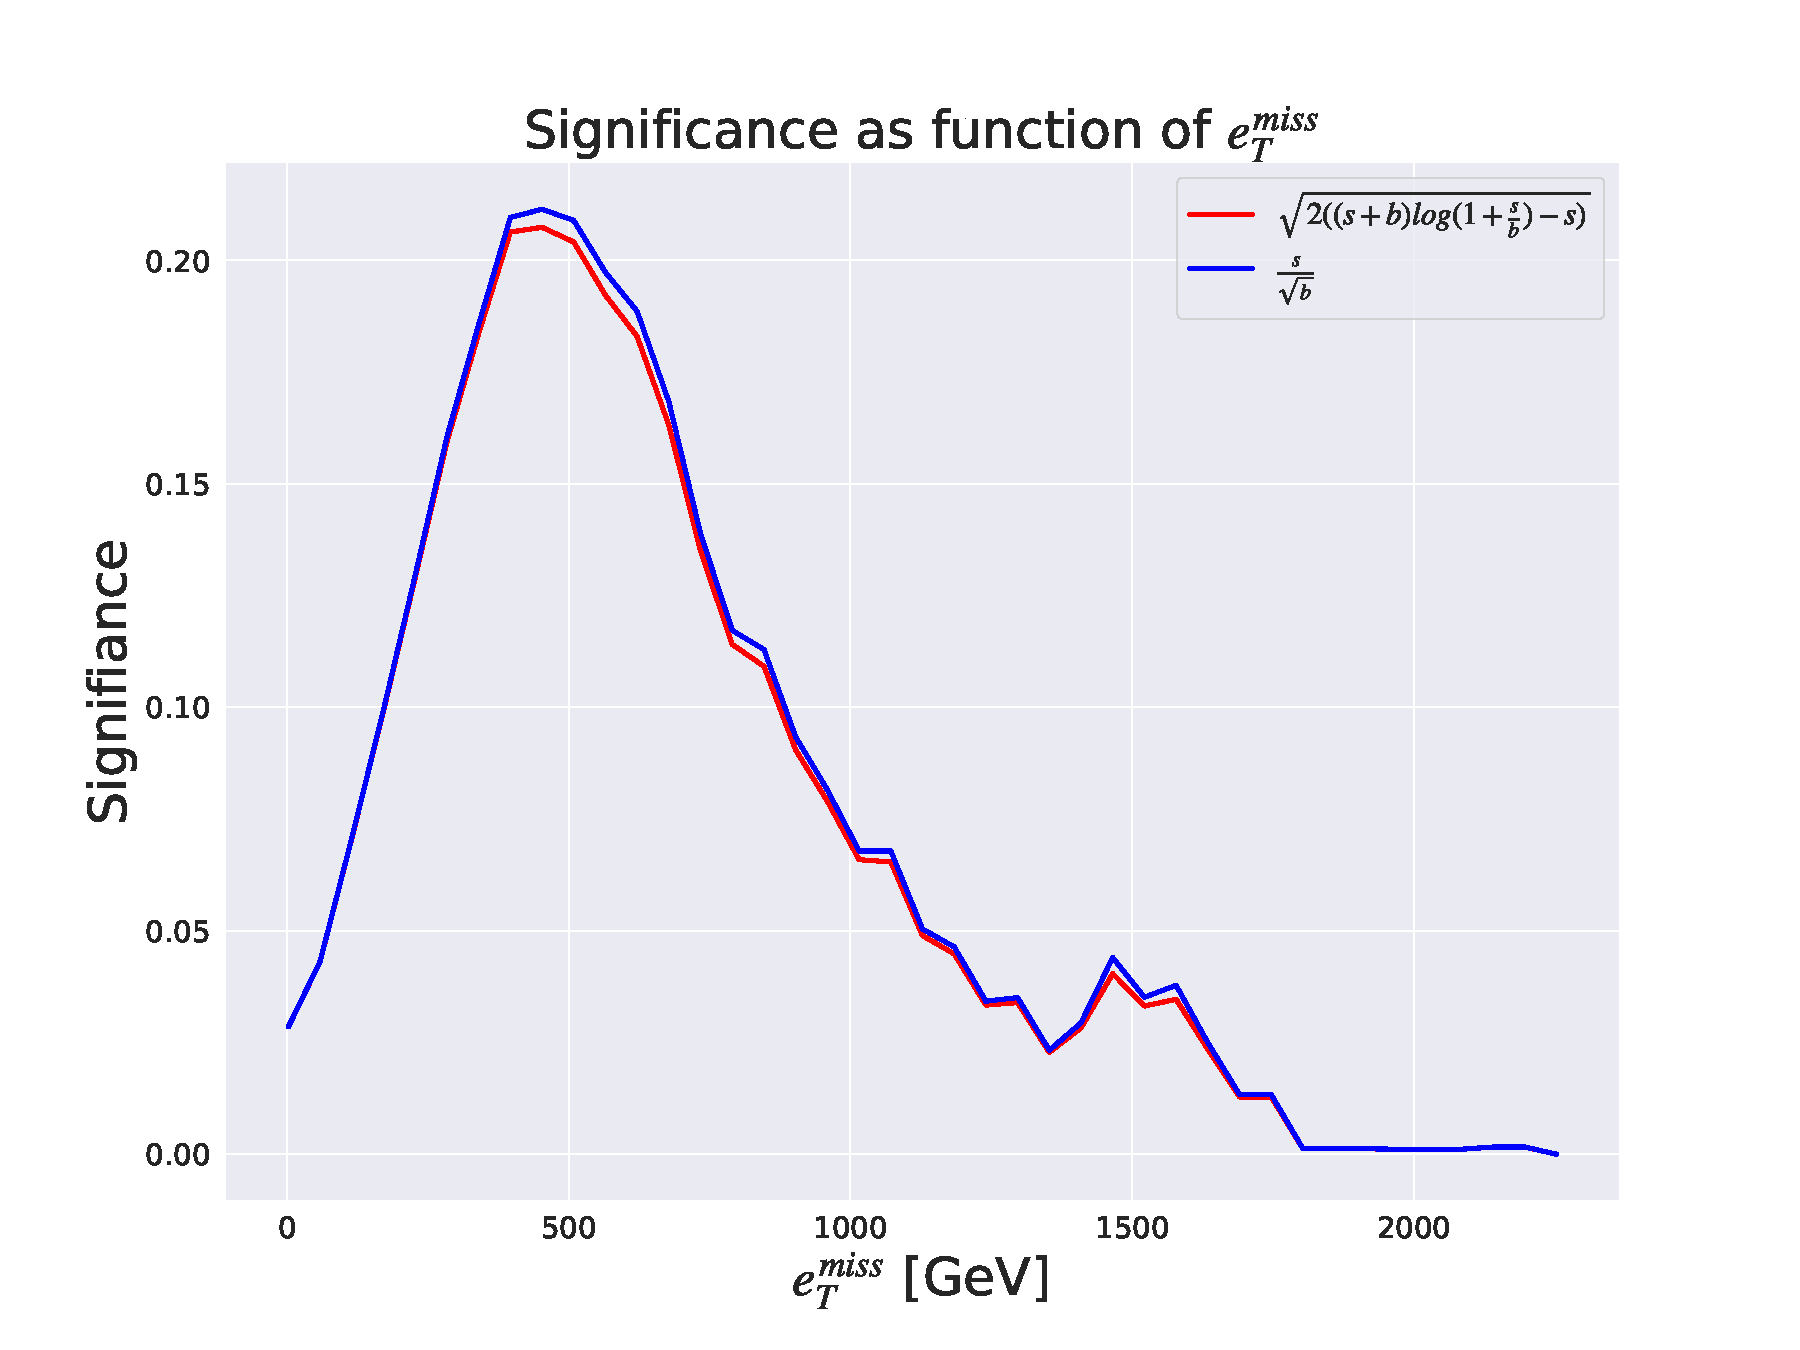
\includegraphics[width=\textwidth]{Figures/AE_testing/big/3lep/significance_etmiss_800p0p050p_-0.9544944422260757.pdf}
        \caption{}
        \label{fig:AE_3lep_big_signi_800_2}
    \end{subfigure}
    \hfill      
    \caption[3lep deep network | $800p50$ | AE | 2]{Reconstruction error, $e_T^{miss}$ signal region, $m_{lll}$ signal region and significance as function of 
    $e_T^{miss}$ for the deep regular autoencoder. Here the SUSY $450p300$ model is used.
    Figure \ref{fig:AE_3lep_big_800_2} shows the reconstruction error 
    distribution for the SM MC and the SUSY signal. Here the autoencoder produce a mirrored reconstruction error shape for both background and 
    signal. Figure \ref{fig:AE_3lep_big_etmiss_800_2} shows the $e_T^{miss}$ distribution for the SM MC and the SUSY signal in the signal region. 
    The signal region is made using a cut around $10^{-0.95}$. Most of the background is removed, with almost no signal in the signal region.
    Figure \ref{fig:AE_3lep_big_mlll_800_2} shows the $m_{lll}$ distribution for the SM MC and the SUSY signal. 
    There is almost no signal in the signal region. Figure \ref{fig:AE_3lep_big_signi_800_2} shows the significance as function of
    $e_T^{miss}$. The peak is put around a cut of about 480 GeV in the $e_T^{miss}$, with a significance of around $0.25$.}
    \label{fig:AE_3lep_big_rec_sig_signi_800_2}
\end{figure}

\begin{figure}[H]
    \centering
    \begin{subfigure}{.40\textwidth}
        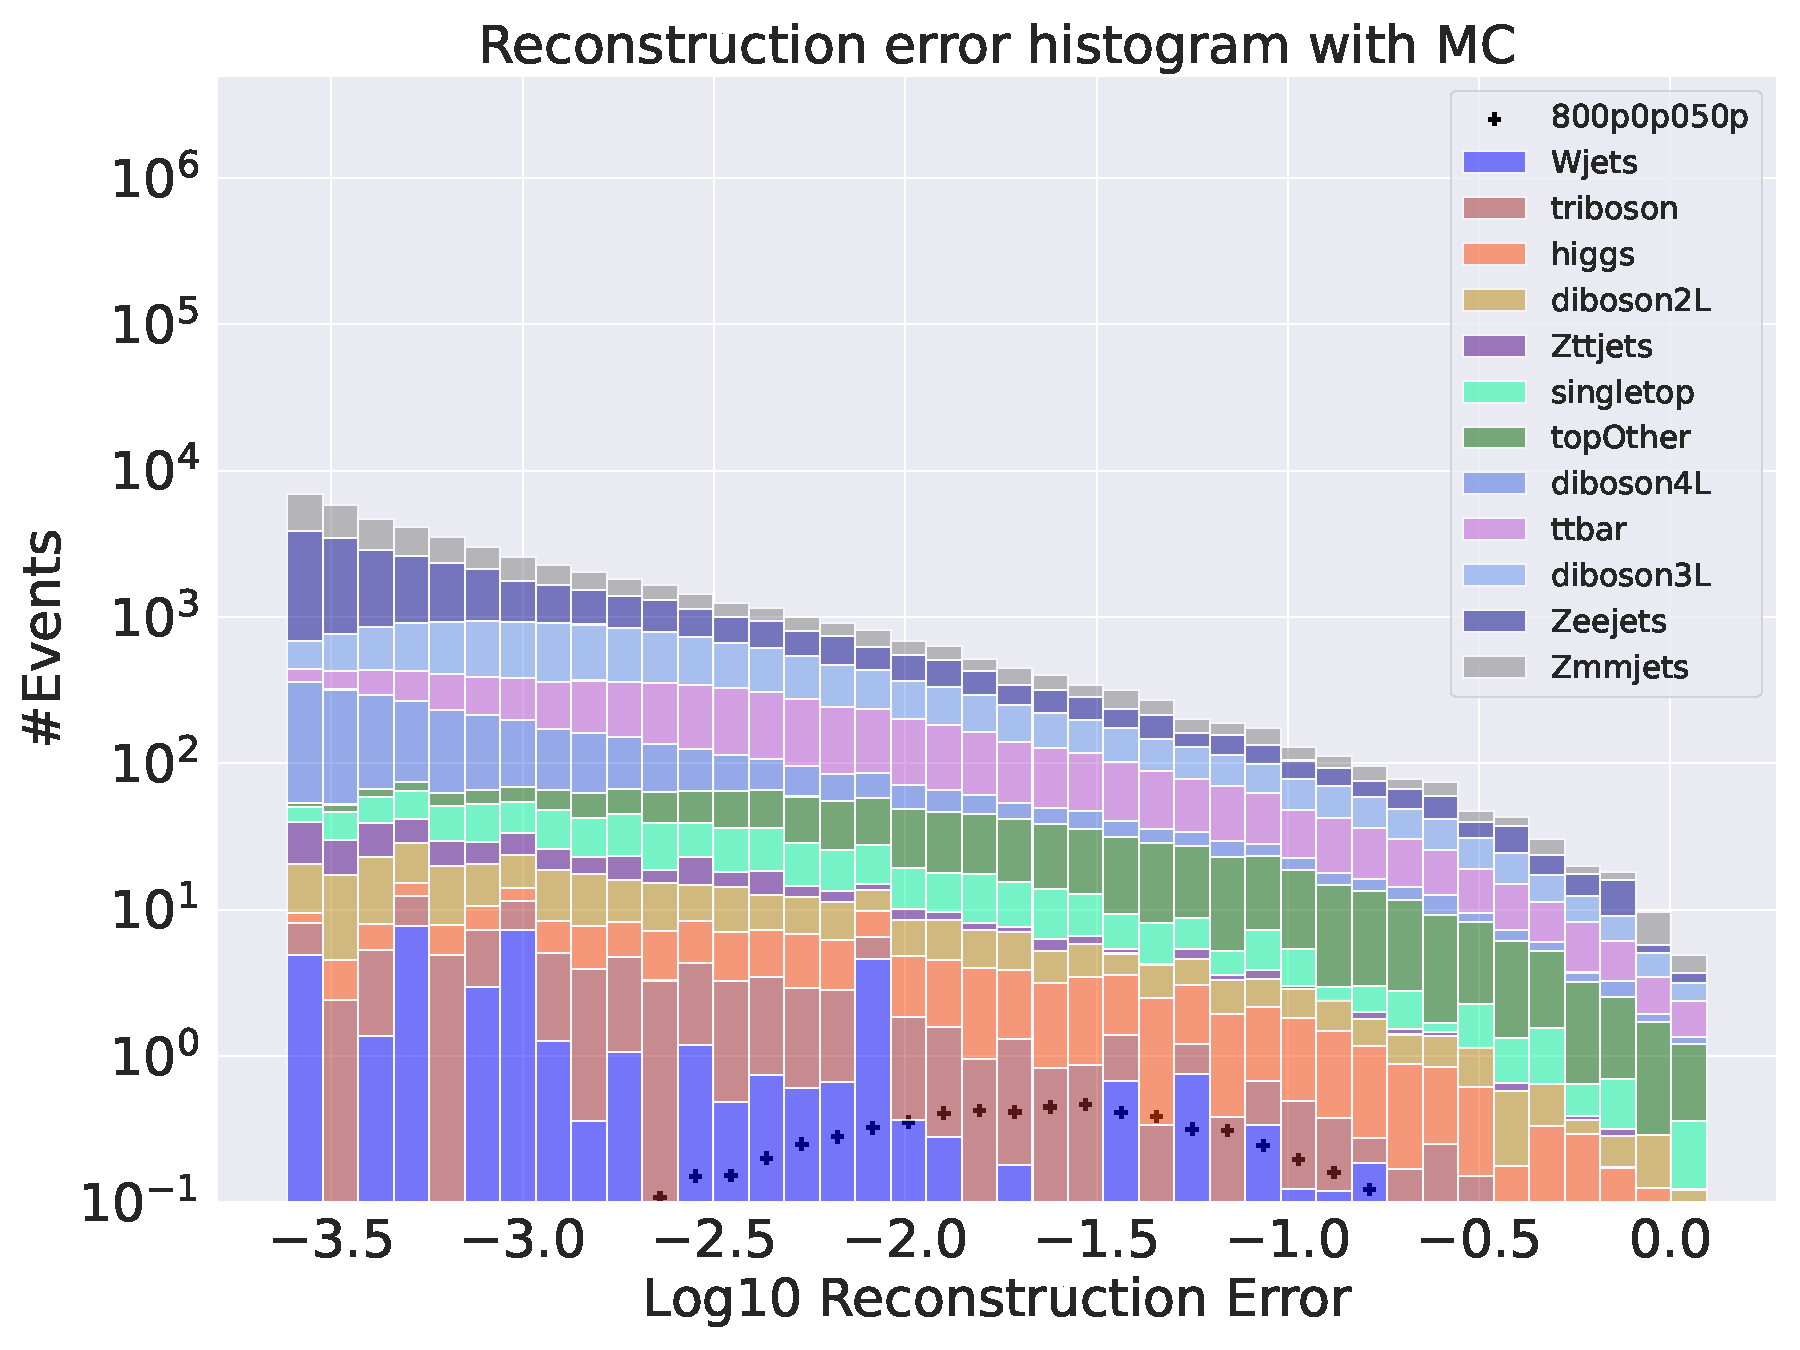
\includegraphics[width=\textwidth]{Figures/AE_testing/small/3lep/b_data_recon_big_rm3_feats_sig_800p0p050p.pdf}
        \caption{ }
        \label{fig:AE_3lep_small_800_2}
    \end{subfigure}
    \hfill
    \begin{subfigure}{.40\textwidth}
        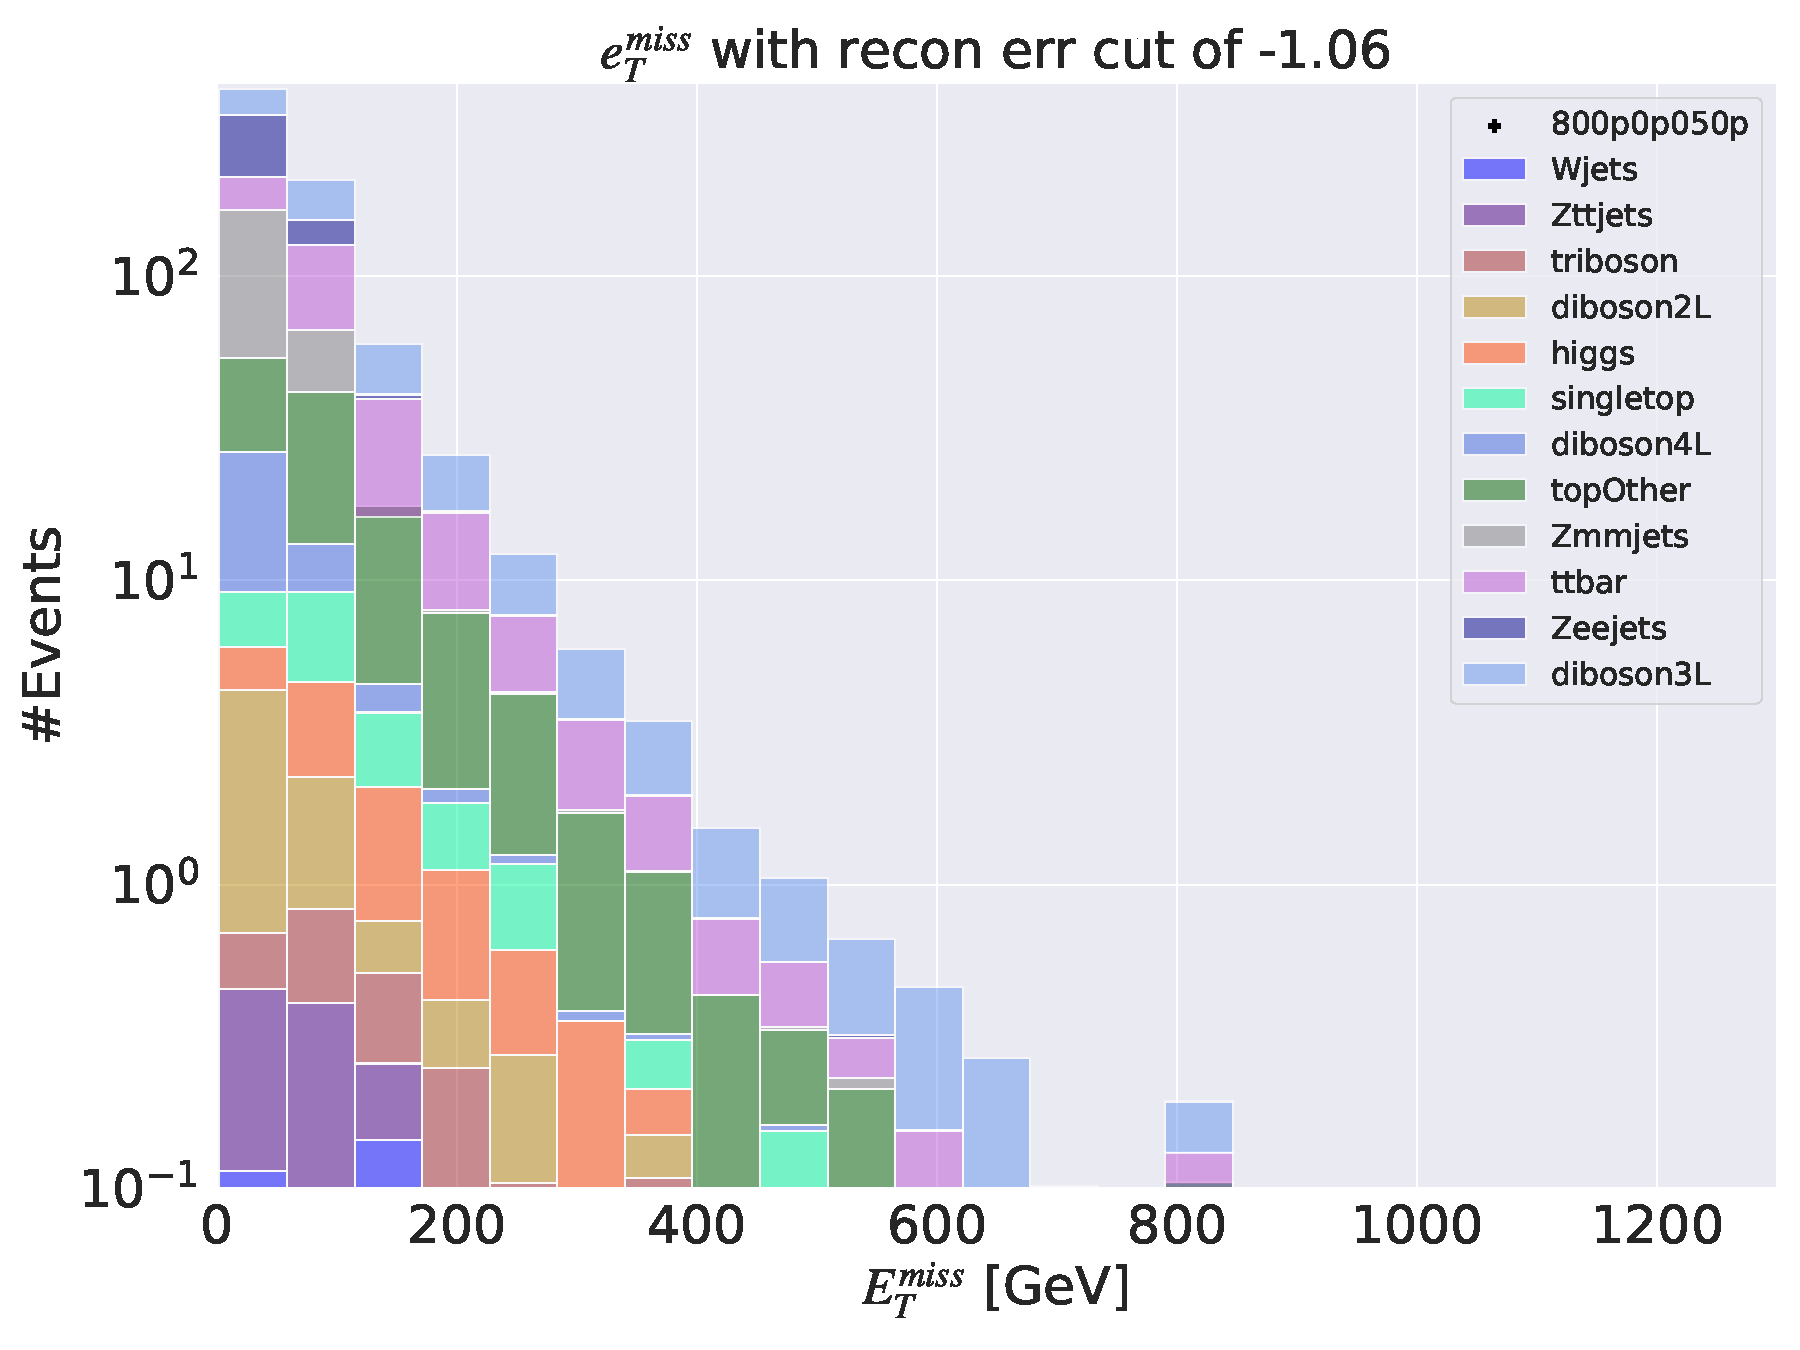
\includegraphics[width=\textwidth]{Figures/AE_testing/small/3lep/b_data_recon_big_rm3_feats_sig_800p0p050p_etmiss_recon_errcut_-1.06.pdf}
        \caption{}
        \label{fig:AE_3lep_small_etmiss_800_2}
    \end{subfigure}
    \hfill
    \begin{subfigure}{.40\textwidth}
        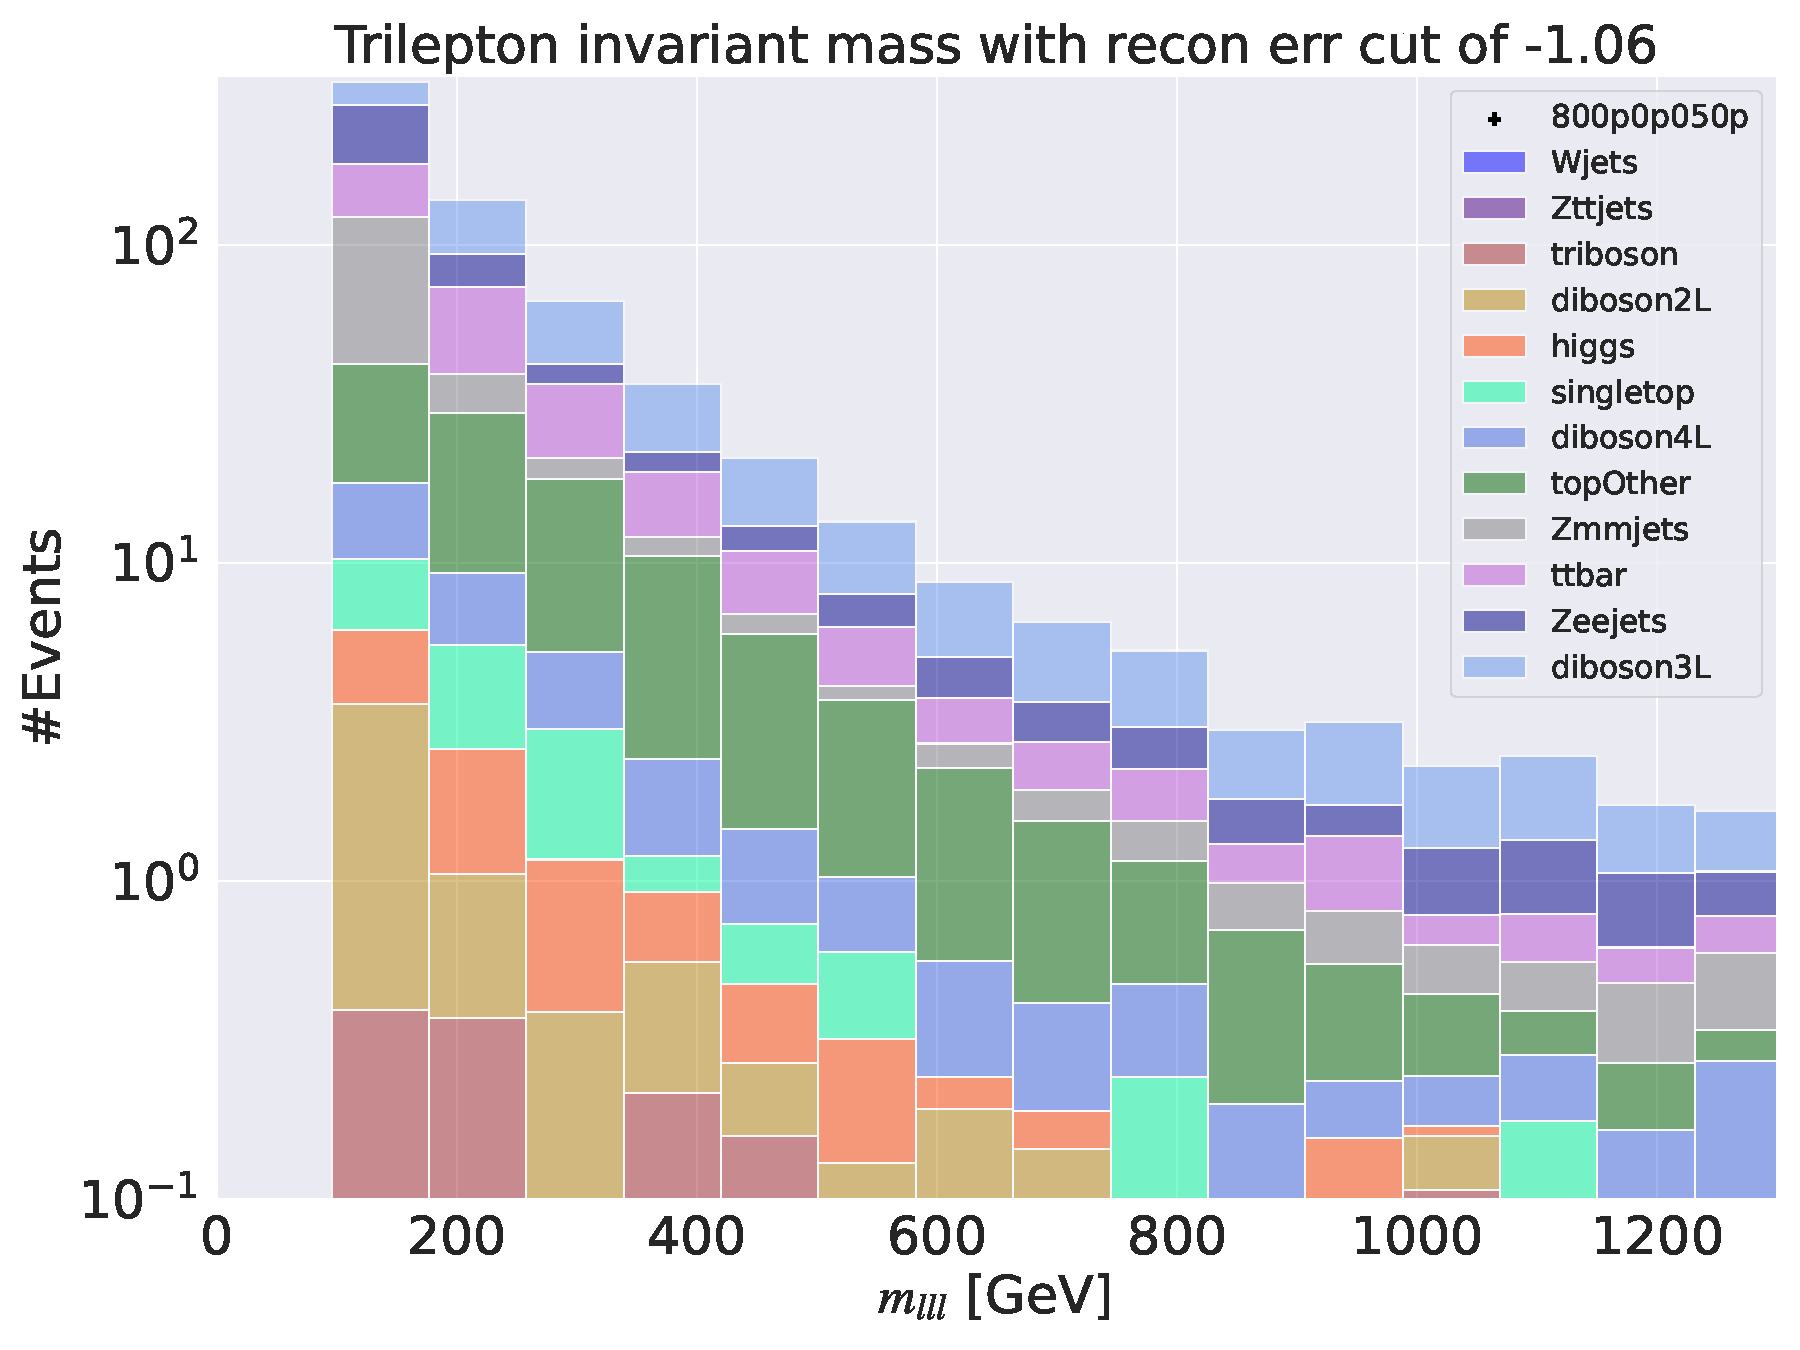
\includegraphics[width=\textwidth]{Figures/AE_testing/small/3lep/b_data_recon_big_rm3_feats_sig_800p0p050p_mlll_recon_errcut_-1.06.pdf}
        \caption{}
        \label{fig:AE_3lep_small_mlll_800_2}
    \end{subfigure}
    \hfill   
    \begin{subfigure}{.40\textwidth}
        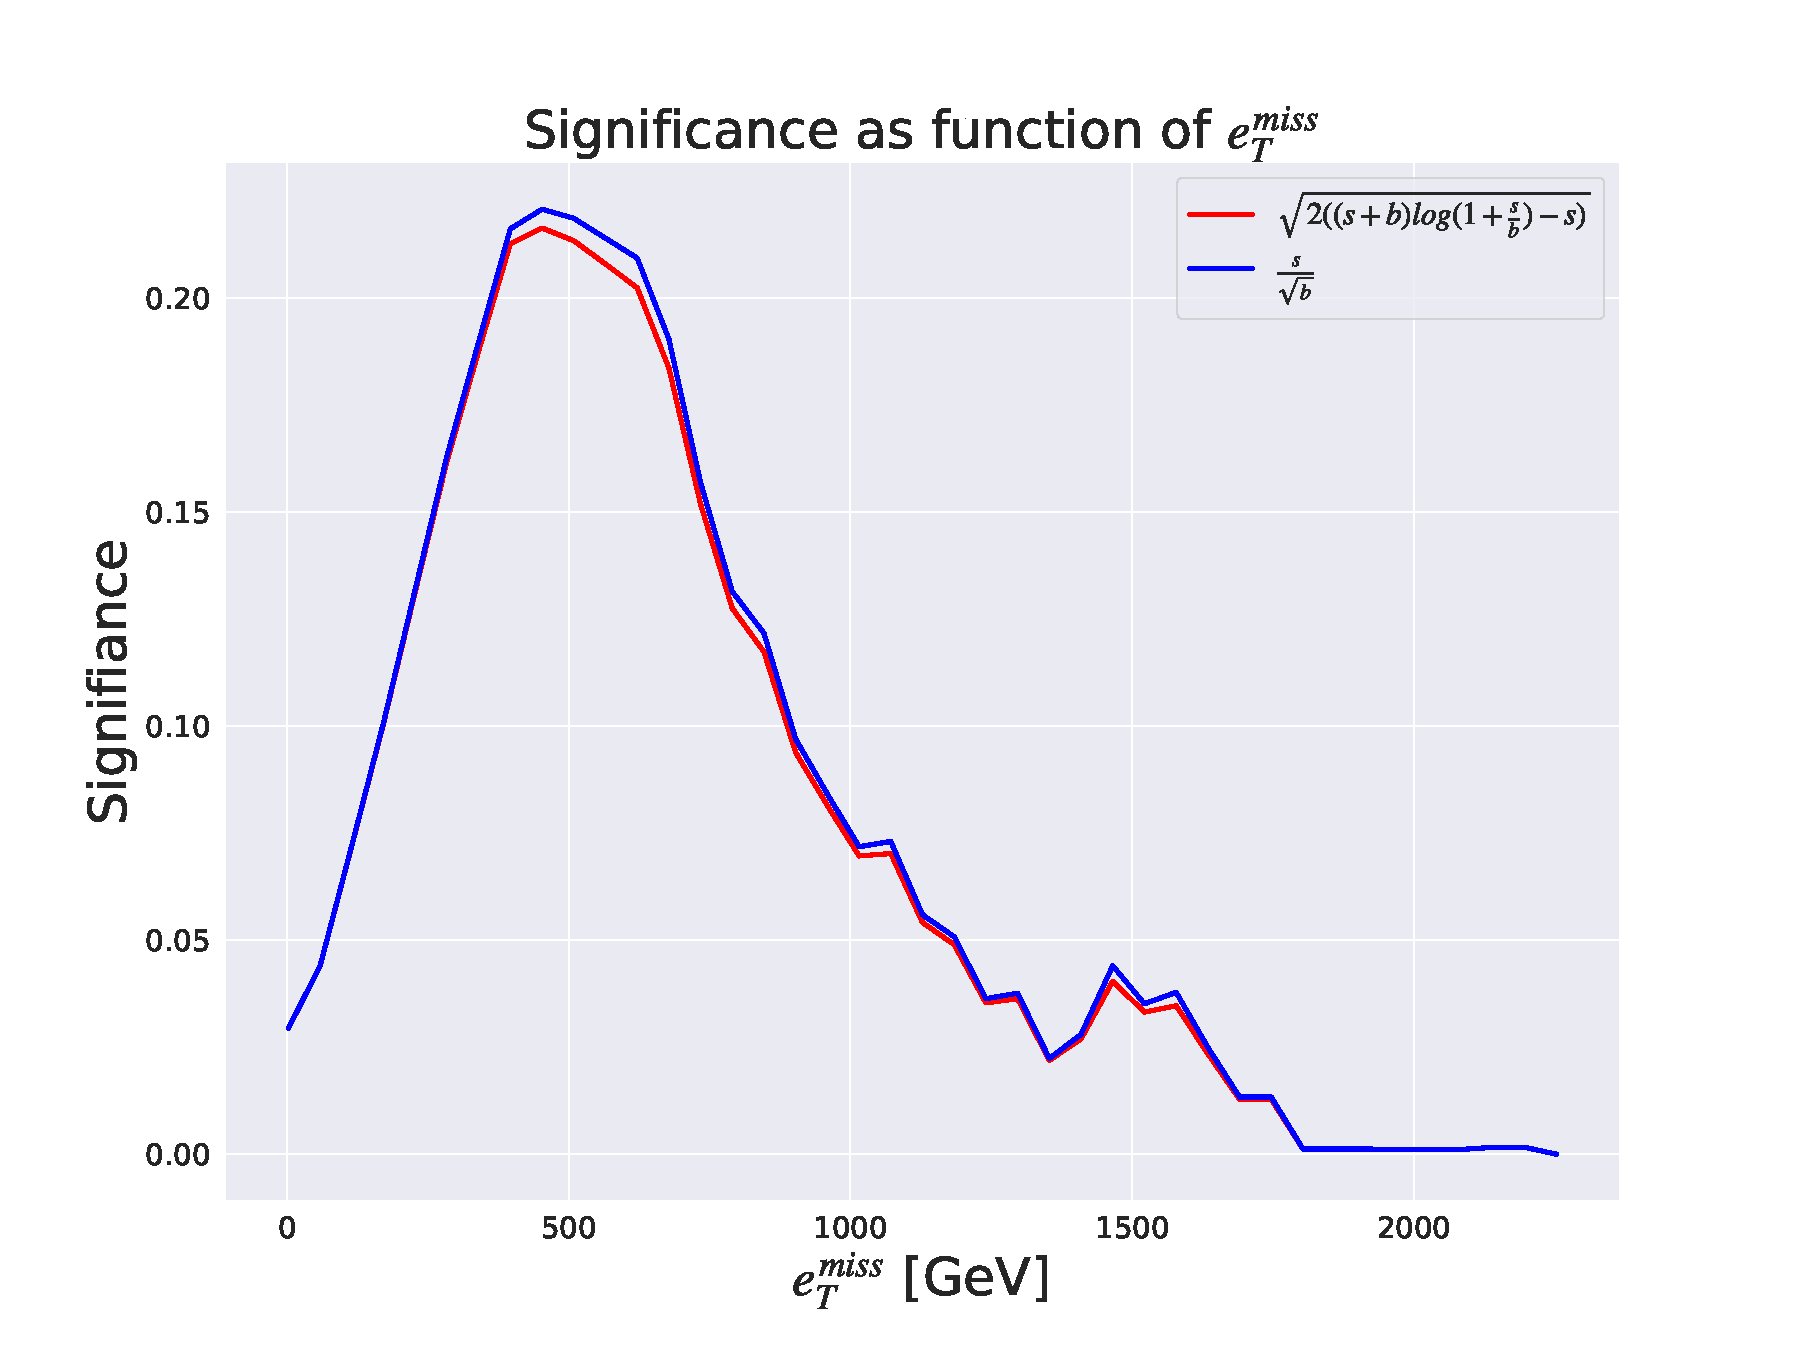
\includegraphics[width=\textwidth]{Figures/AE_testing/small/3lep/significance_etmiss_800p0p050p_-1.0567039801896674.pdf}
        \caption{}
        \label{fig:AE_3lep_small_signi_800_2}
    \end{subfigure}
    \hfill      
    \caption[3lep shallow network | $800p50$ | AE | 2]{Reconstruction error, $e_T^{miss}$ signal region, $m_{lll}$ signal region and significance as function of 
    $e_T^{miss}$ for the shallow regular autoencoder. Here the SUSY $450p300$ model is used. 
    Figure \ref{fig:AE_3lep_small_800_2} shows the reconstruction error 
    distribution for the SM MC and the SUSY signal. Here the autoencoder produce a mirrored reconstruction error shape for both background and 
    signal. Figure \ref{fig:AE_3lep_small_etmiss_800_2} shows the $e_T^{miss}$ distribution for the SM MC and the SUSY signal in the signal region. 
    The signal region is made using a cut around $10^{-1.06}$. Most of the background is removed, with almost no signal in the signal region.
    Figure \ref{fig:AE_3lep_small_mlll_800_2} shows the $m_{lll}$ distribution for the SM MC and the SUSY signal. 
    There is almost no signal in the signal region. Figure \ref{fig:AE_3lep_small_signi_800_2} shows the significance as function of
    $e_T^{miss}$. The peak is put around a cut of about 480 GeV in the $e_T^{miss}$, with a significance of around $0.23$.}
    \label{fig:AE_3lep_small_rec_sig_signi_800_2}
\end{figure}












\begin{figure}[H]
    \centering
    \begin{subfigure}{.40\textwidth}
        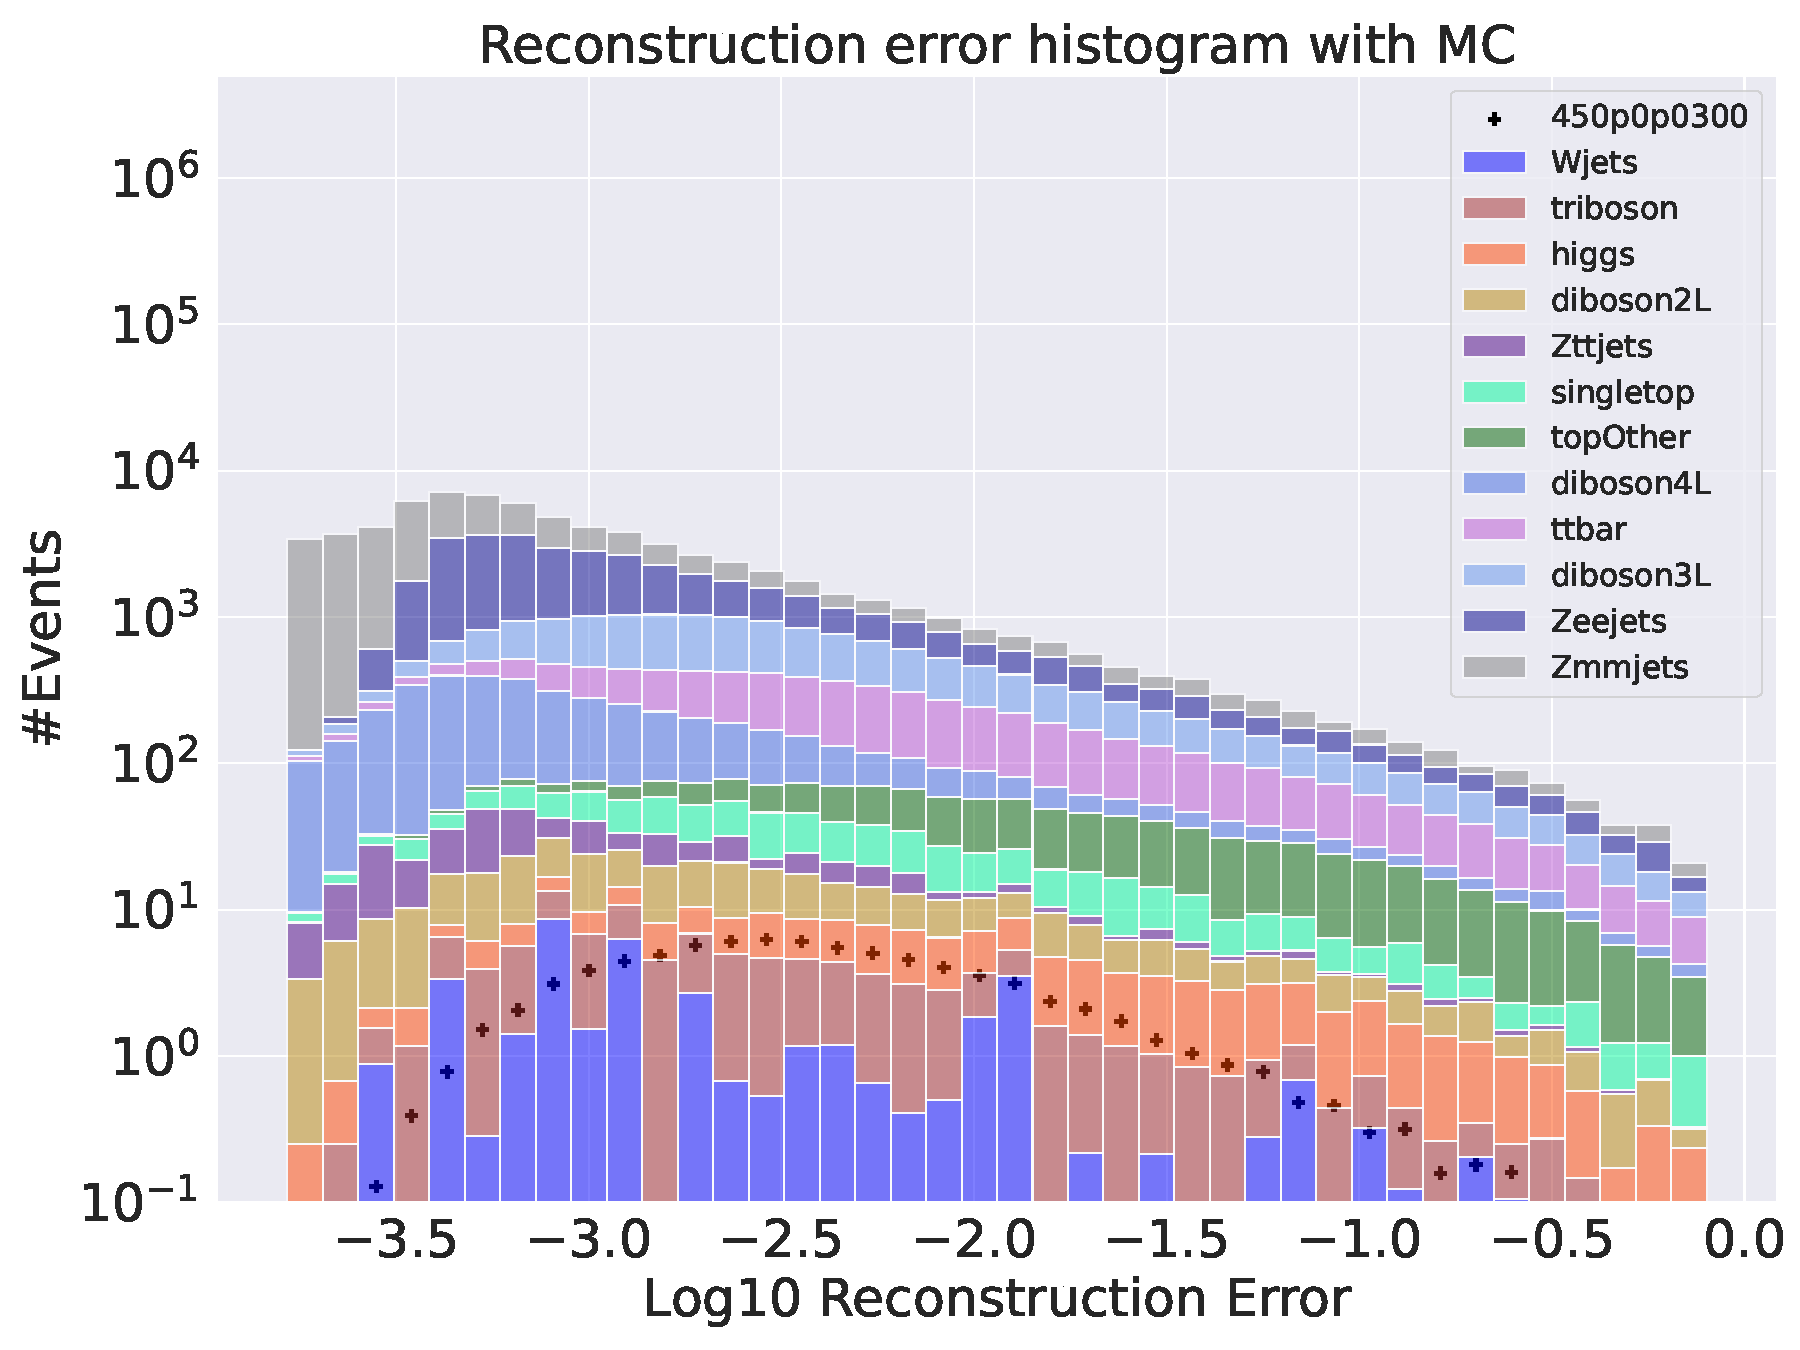
\includegraphics[width=\textwidth]{Figures/AE_testing/big/3lep/b_data_recon_big_rm3_feats_sig_450p0p0300.pdf}
        \caption{ }
        \label{fig:AE_3lep_big_450_3}
    \end{subfigure}
    \hfill
    \begin{subfigure}{.40\textwidth}
        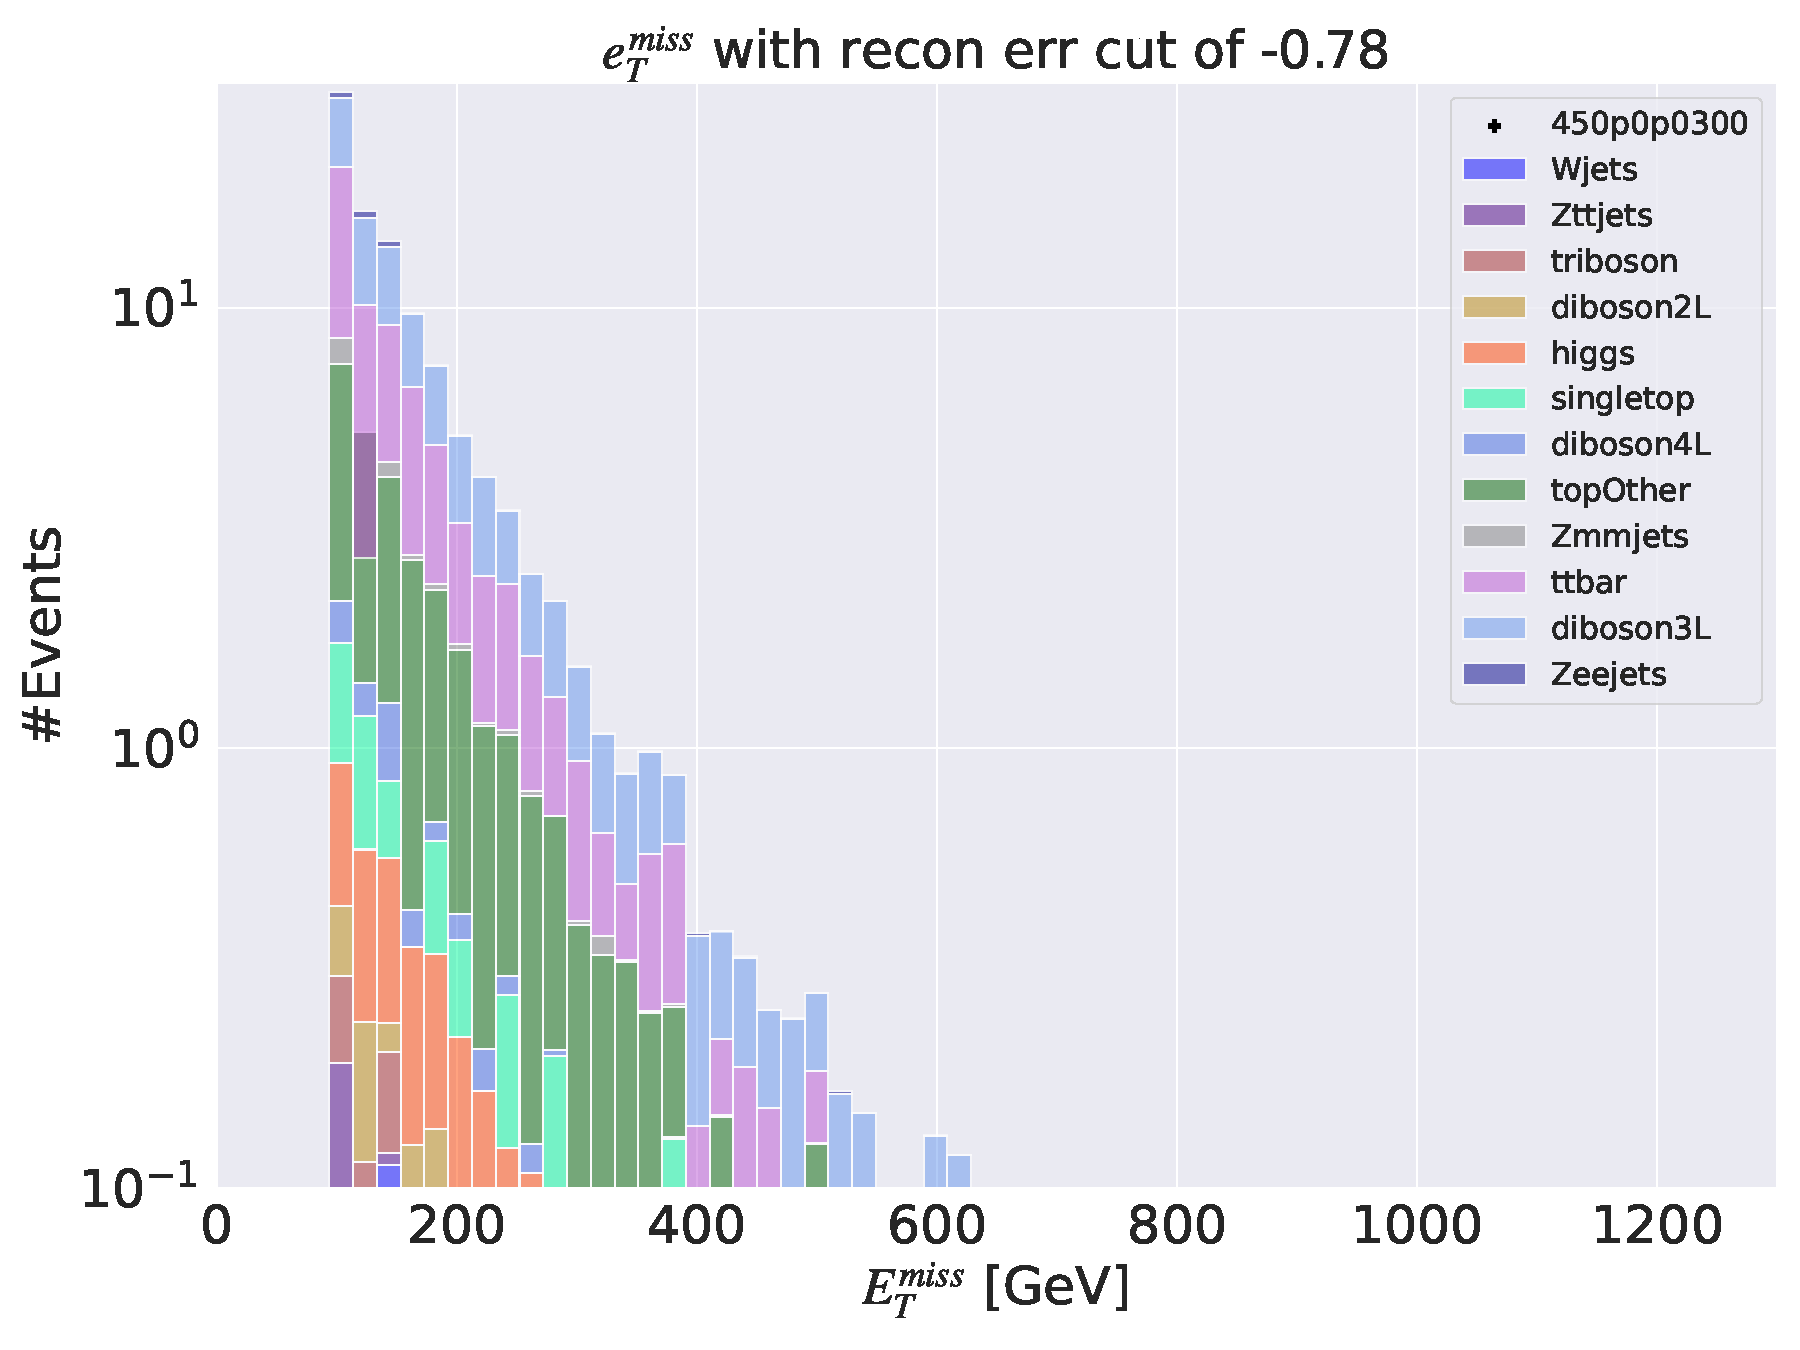
\includegraphics[width=\textwidth]{Figures/AE_testing/big/3lep/b_data_recon_big_rm3_feats_sig_450p0p0300_etmiss_recon_errcut_-0.78.pdf}
        \caption{}
        \label{fig:AE_3lep_big_etmiss_450_3}
    \end{subfigure}
    \hfill
    \begin{subfigure}{.40\textwidth}
        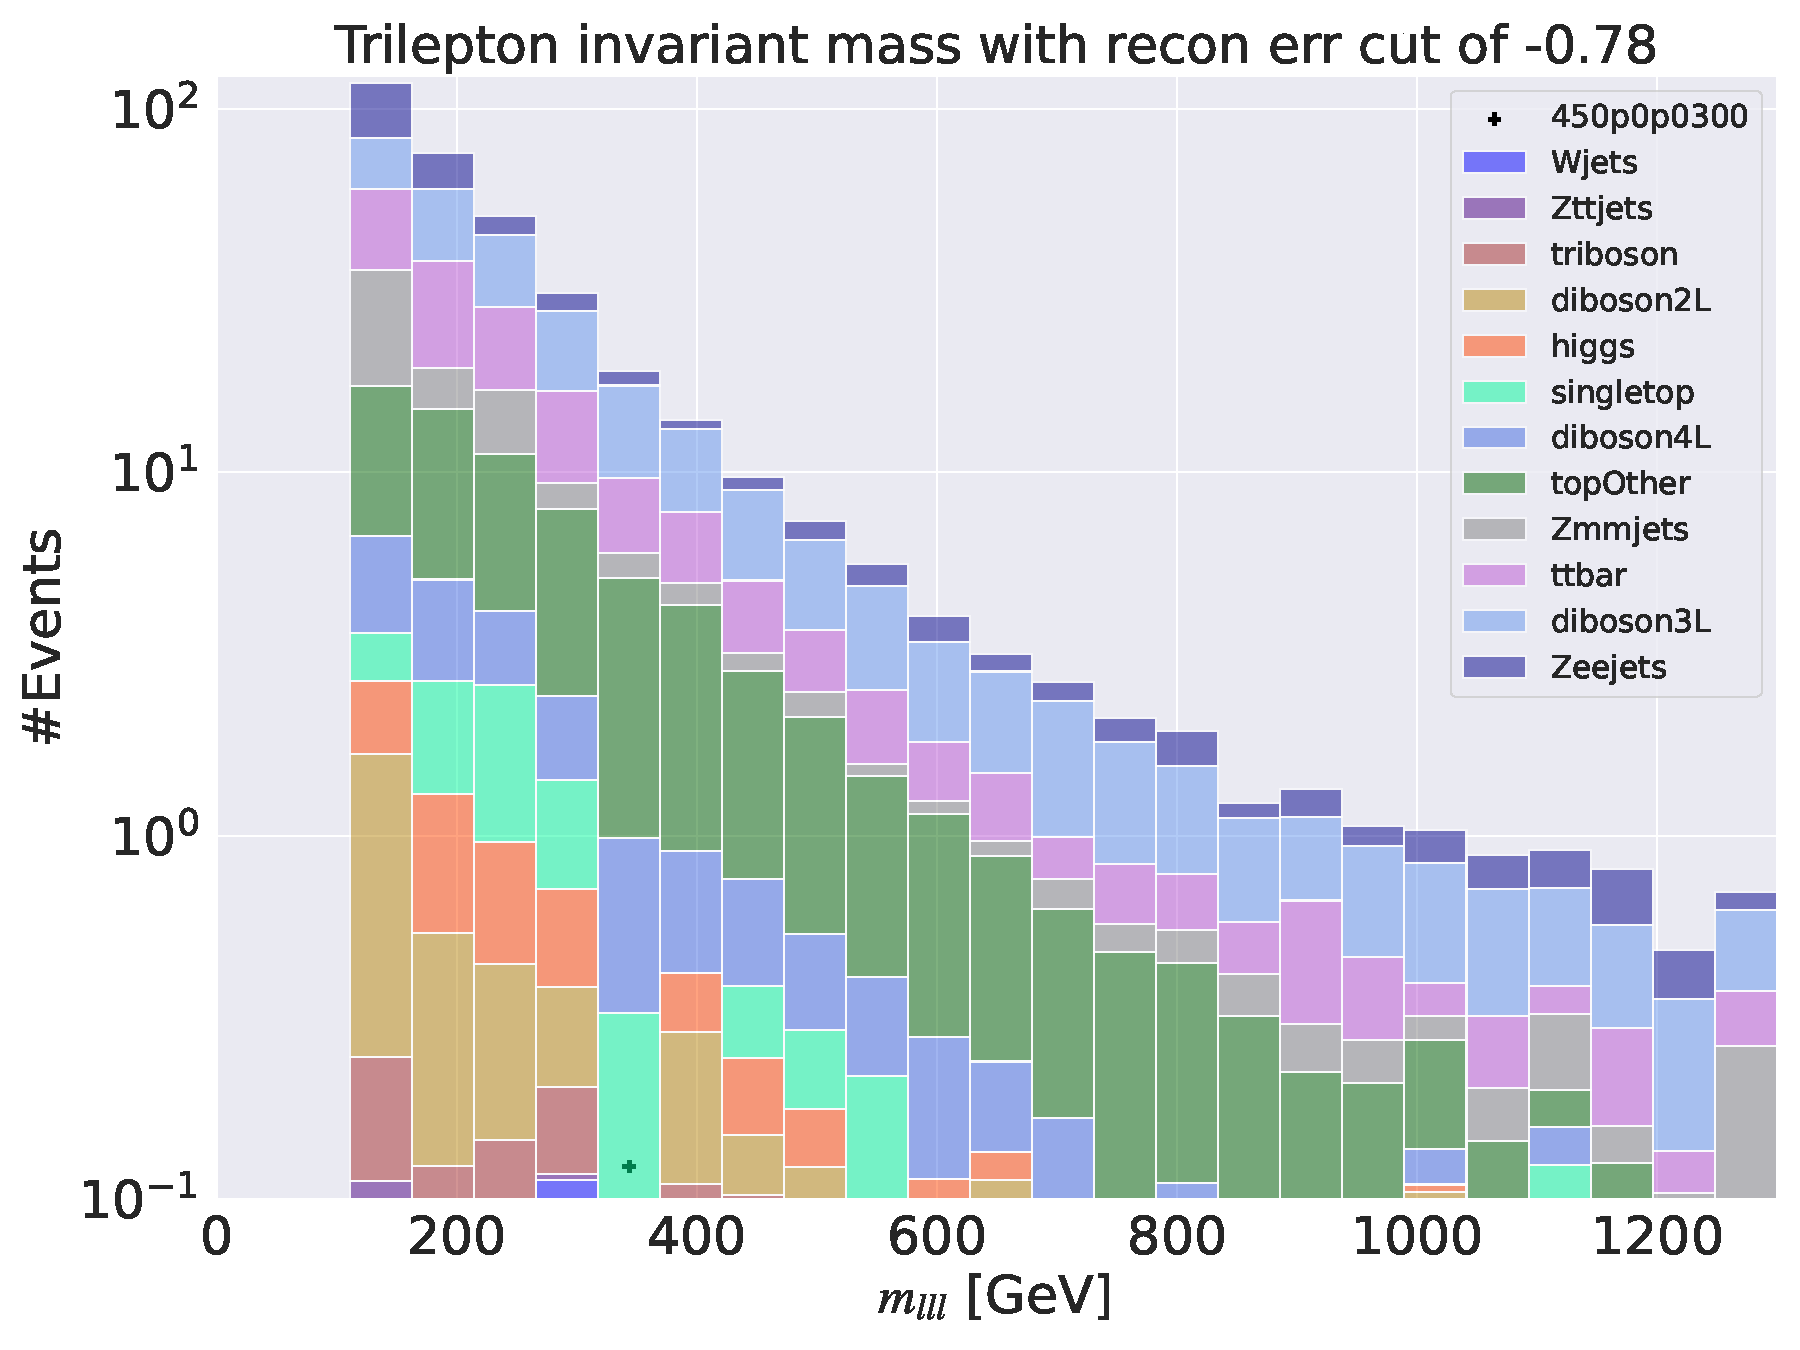
\includegraphics[width=\textwidth]{Figures/AE_testing/big/3lep/b_data_recon_big_rm3_feats_sig_450p0p0300_mlll_recon_errcut_-0.78.pdf}
        \caption{}
        \label{fig:AE_3lep_big_mlll_450_3}
    \end{subfigure}
    \hfill   
    \begin{subfigure}{.40\textwidth}
        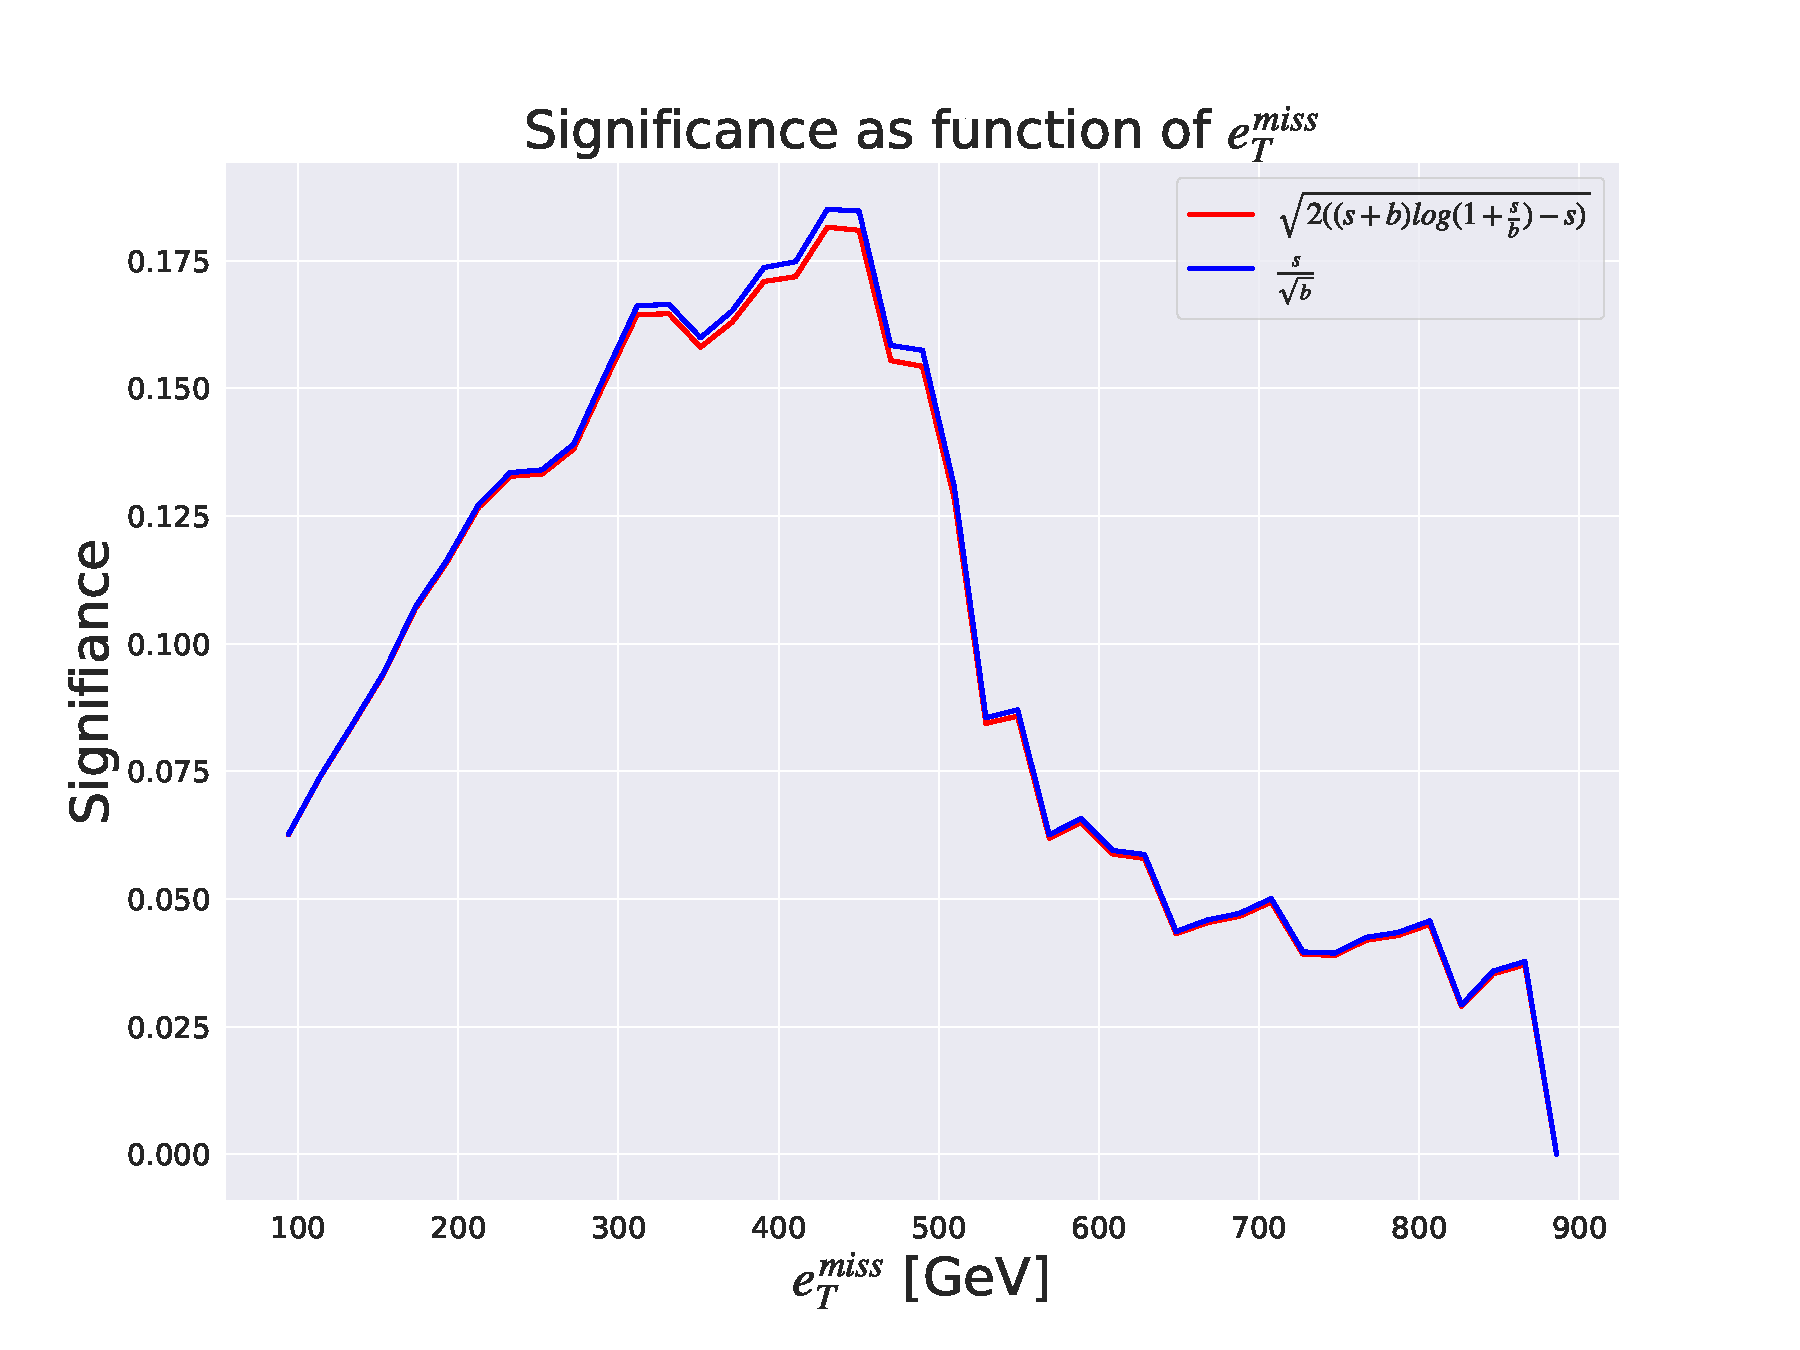
\includegraphics[width=\textwidth]{Figures/AE_testing/big/3lep/significance_etmiss_450p0p0300_-0.7824137709201433.pdf}
        \caption{}
        \label{fig:AE_3lep_big_signi_450_3}
    \end{subfigure}
    \hfill      
    \caption[3lep deep network | $450p300$ | AE | 3]{Reconstruction error, $e_T^{miss}$ signal region, $m_{lll}$ signal region and significance as function of 
    $e_T^{miss}$ for the deep regular autoencoder. Here the SUSY $450p300$ model is used. 
    Figure \ref{fig:AE_3lep_big_450_3} shows the reconstruction error 
    distribution for the SM MC and the SUSY signal. Here the autoencoder produce the same reconstruction error shape for both background and 
    signal. Figure \ref{fig:AE_3lep_big_etmiss_450_3} shows the $e_T^{miss}$ distribution for the SM MC and the SUSY signal in the signal region. 
    The signal region is made using a cut around $10^{-0.78}$. Most of the background is removed, with almost no signal in the signal region.
    Figure \ref{fig:AE_3lep_big_mlll_450_3} shows the $m_{lll}$ distribution for the SM MC and the SUSY signal. 
    There is almost no signal in the signal region. Figure \ref{fig:AE_3lep_big_signi_450_3} shows the significance as function of
    $e_T^{miss}$. The peak is put around a cut of about 430 GeV in the $e_T^{miss}$, with a significance of around $0.185$.}
    \label{fig:AE_3lep_big_rec_sig_signi_450_3}
\end{figure}

\begin{figure}[H]
    \centering
    \begin{subfigure}{.40\textwidth}
        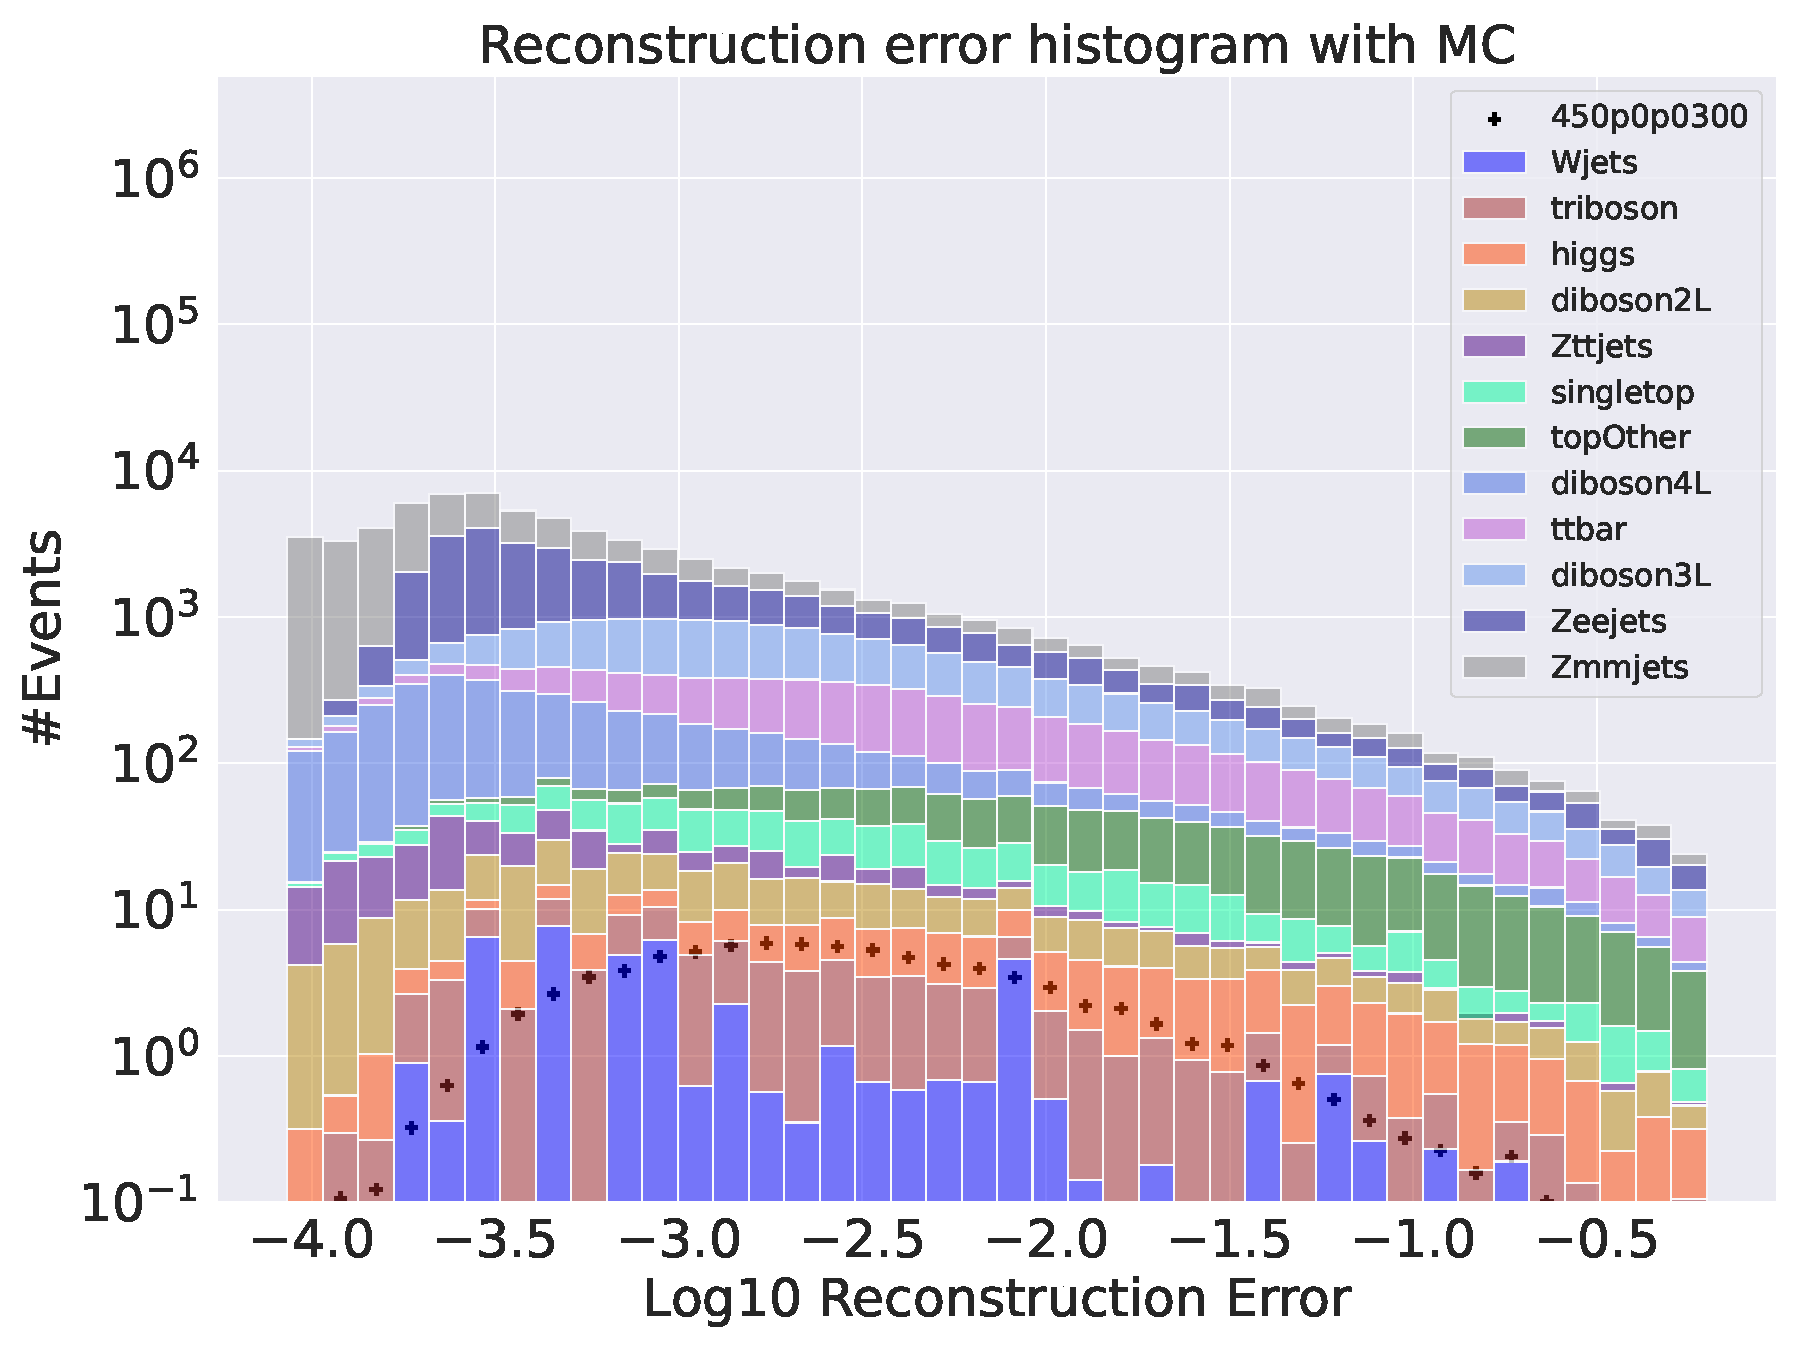
\includegraphics[width=\textwidth]{Figures/AE_testing/small/3lep/b_data_recon_big_rm3_feats_sig_450p0p0300.pdf}
        \caption{ }
        \label{fig:AE_3lep_small_450_3}
    \end{subfigure}
    \hfill
    \begin{subfigure}{.40\textwidth}
        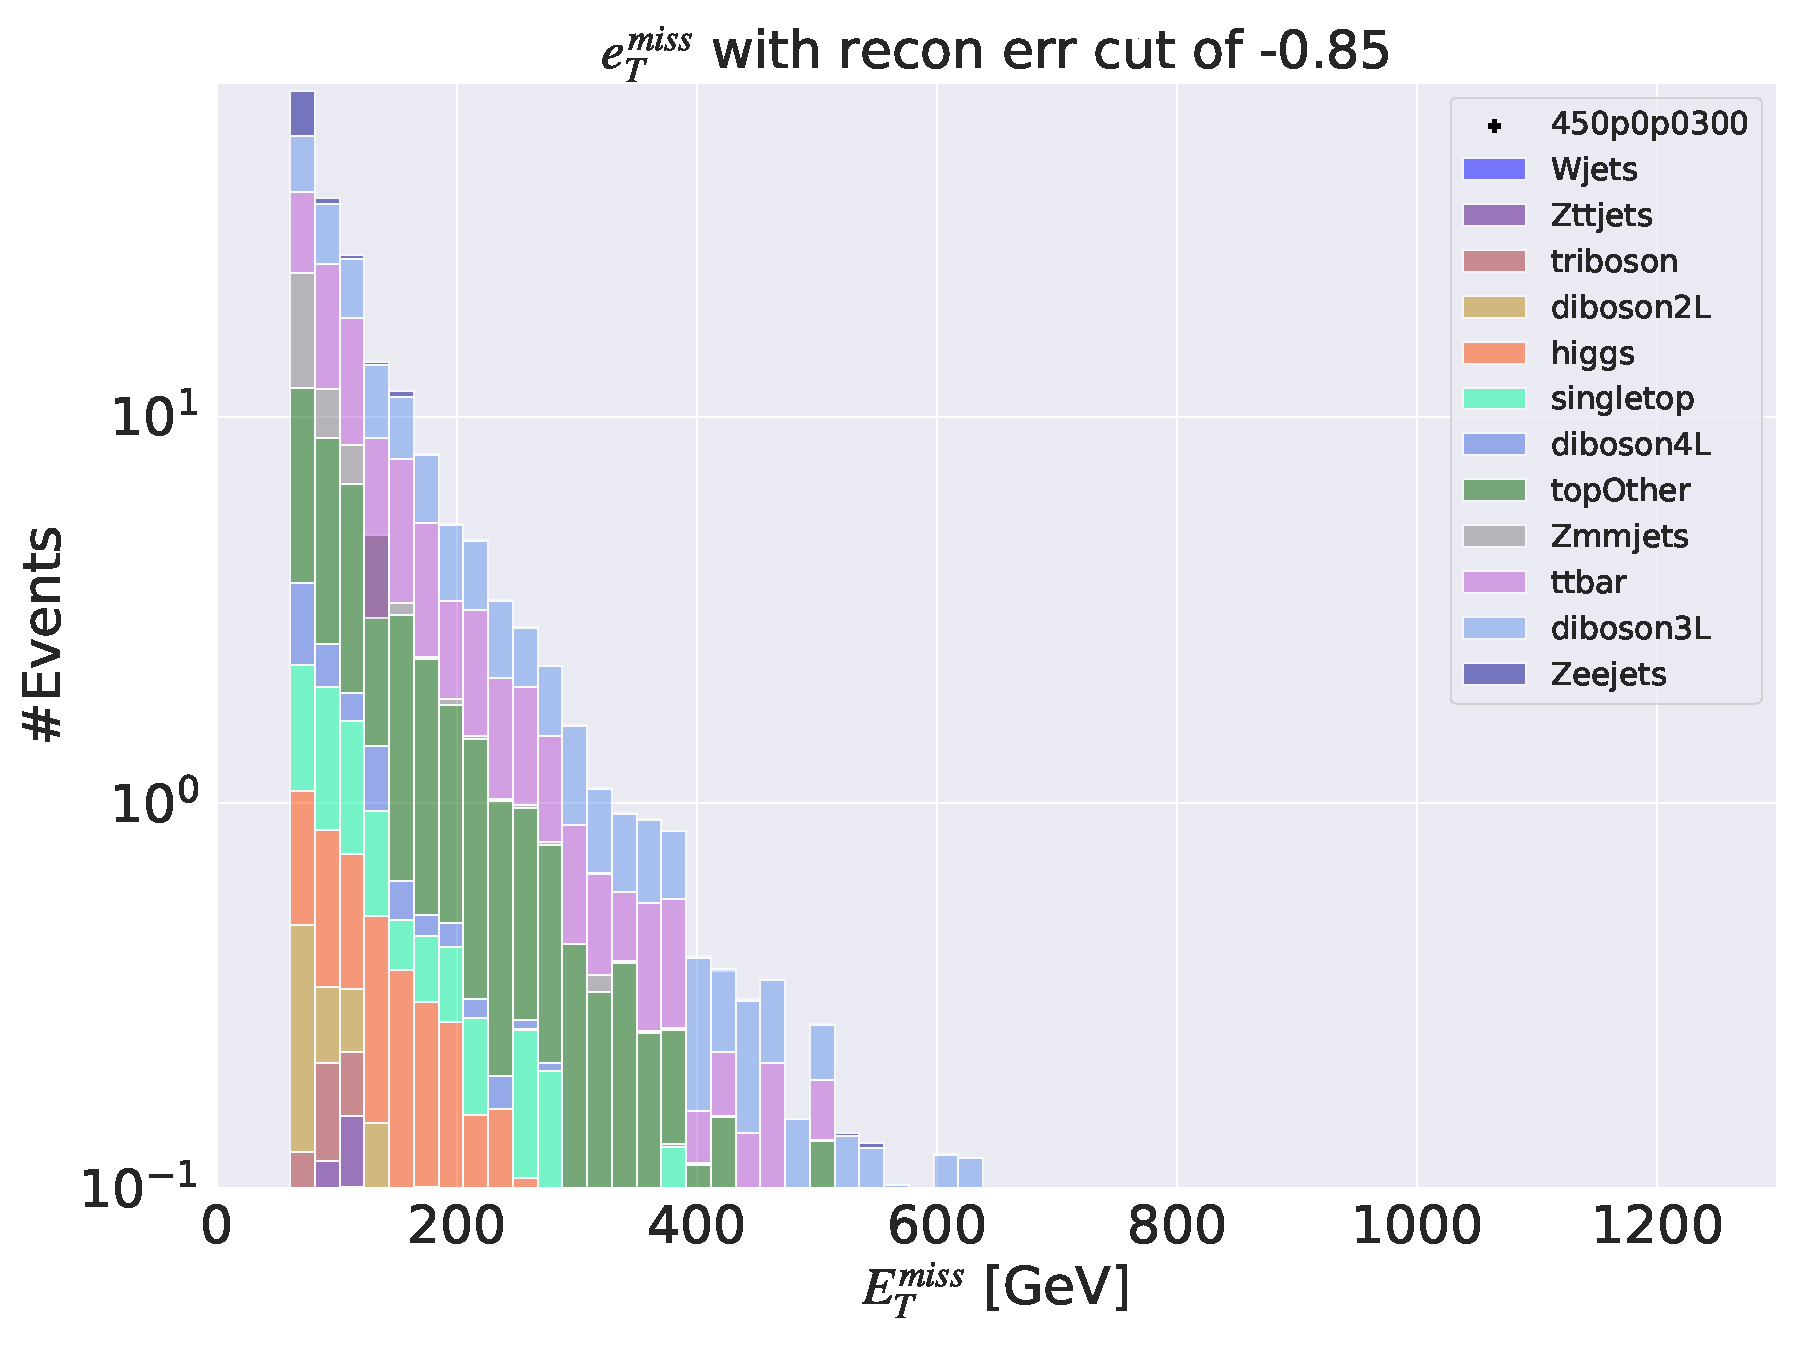
\includegraphics[width=\textwidth]{Figures/AE_testing/small/3lep/b_data_recon_big_rm3_feats_sig_450p0p0300_etmiss_recon_errcut_-0.85.pdf}
        \caption{}
        \label{fig:AE_3lep_small_etmiss_450_3}
    \end{subfigure}
    \hfill
    \begin{subfigure}{.40\textwidth}
        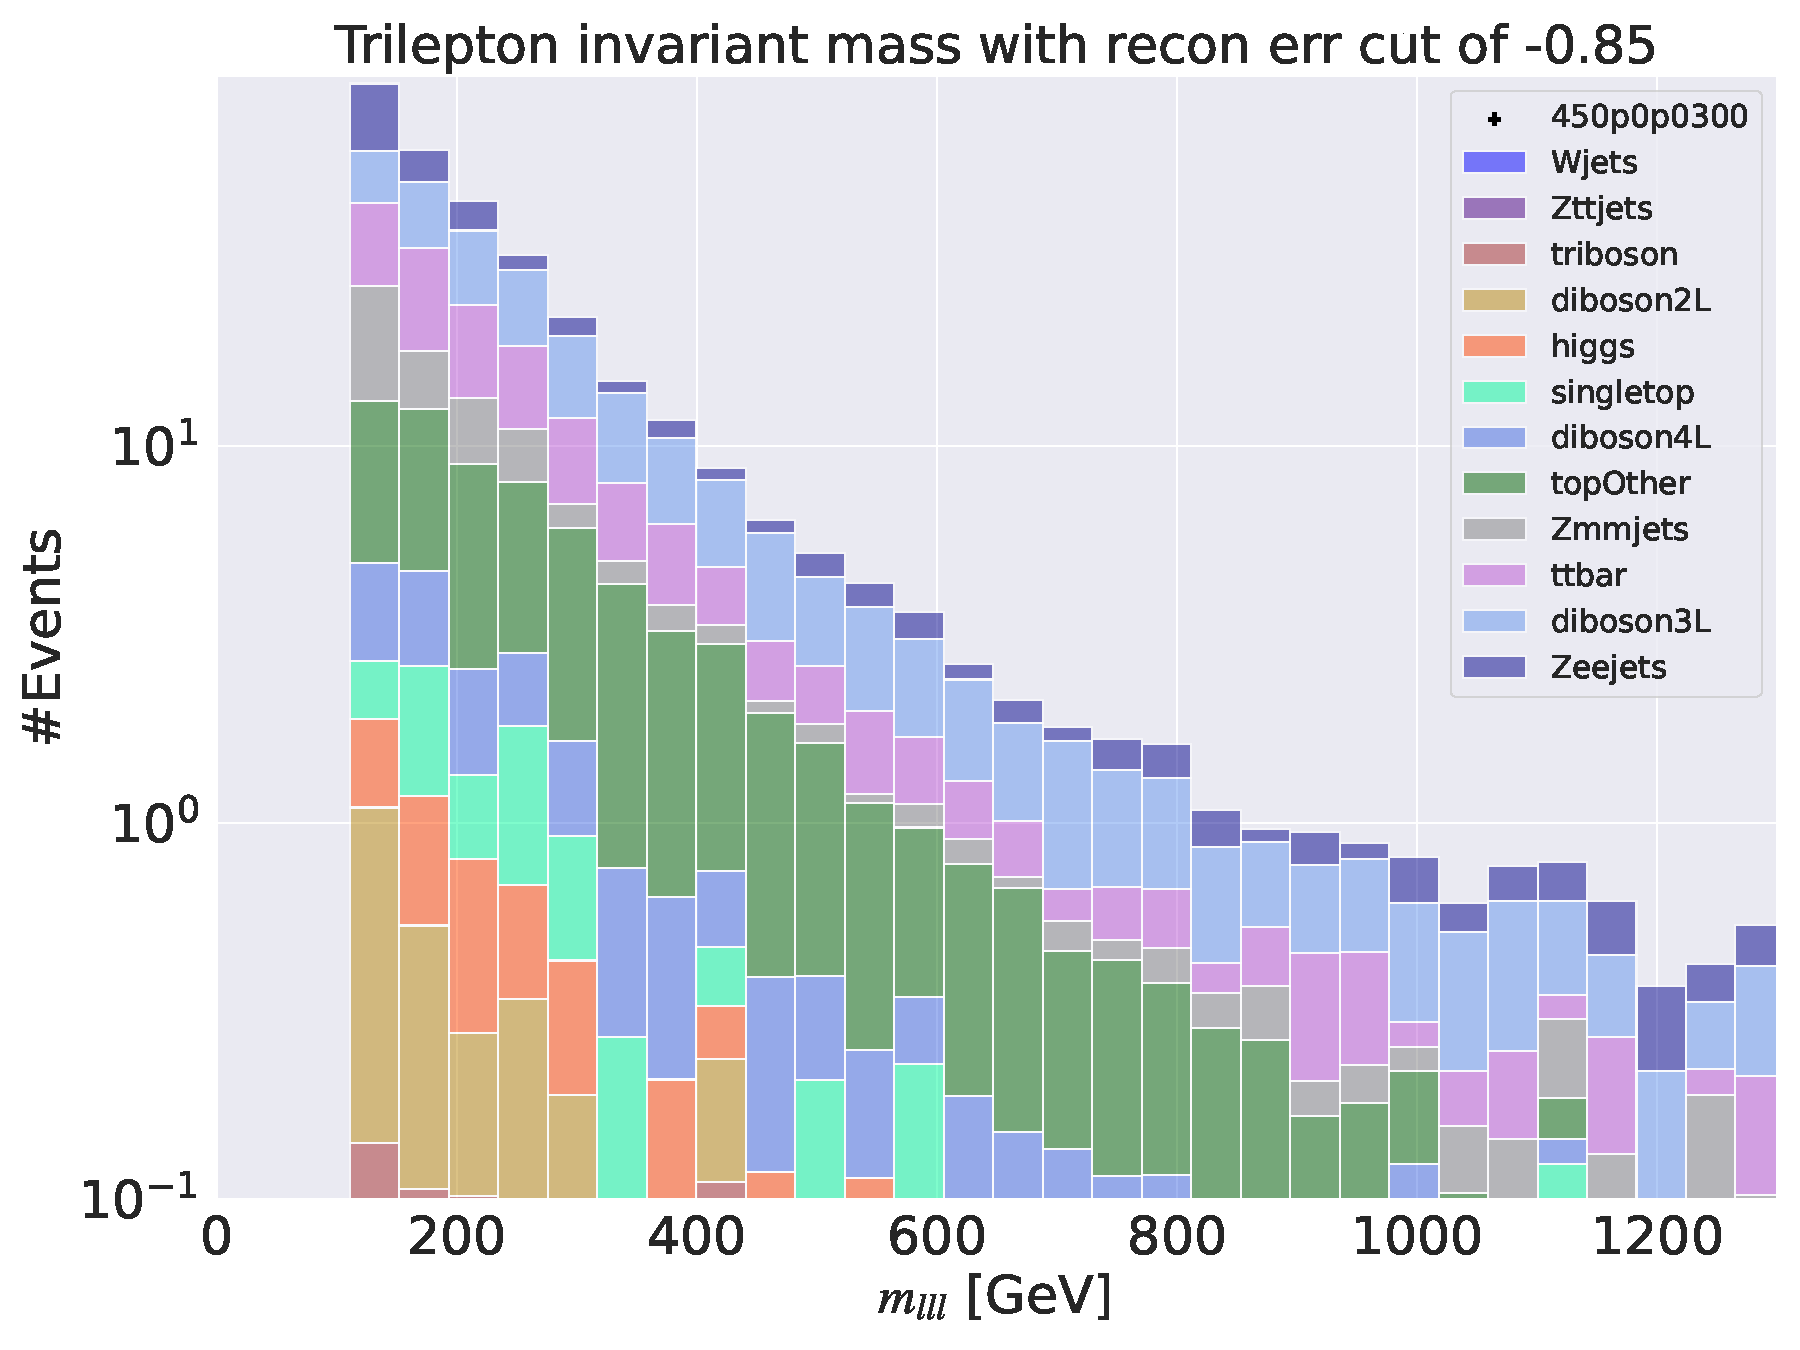
\includegraphics[width=\textwidth]{Figures/AE_testing/small/3lep/b_data_recon_big_rm3_feats_sig_450p0p0300_mlll_recon_errcut_-0.85.pdf}
        \caption{}
        \label{fig:AE_3lep_small_mlll_450_3}
    \end{subfigure}
    \hfill   
    \begin{subfigure}{.40\textwidth}
        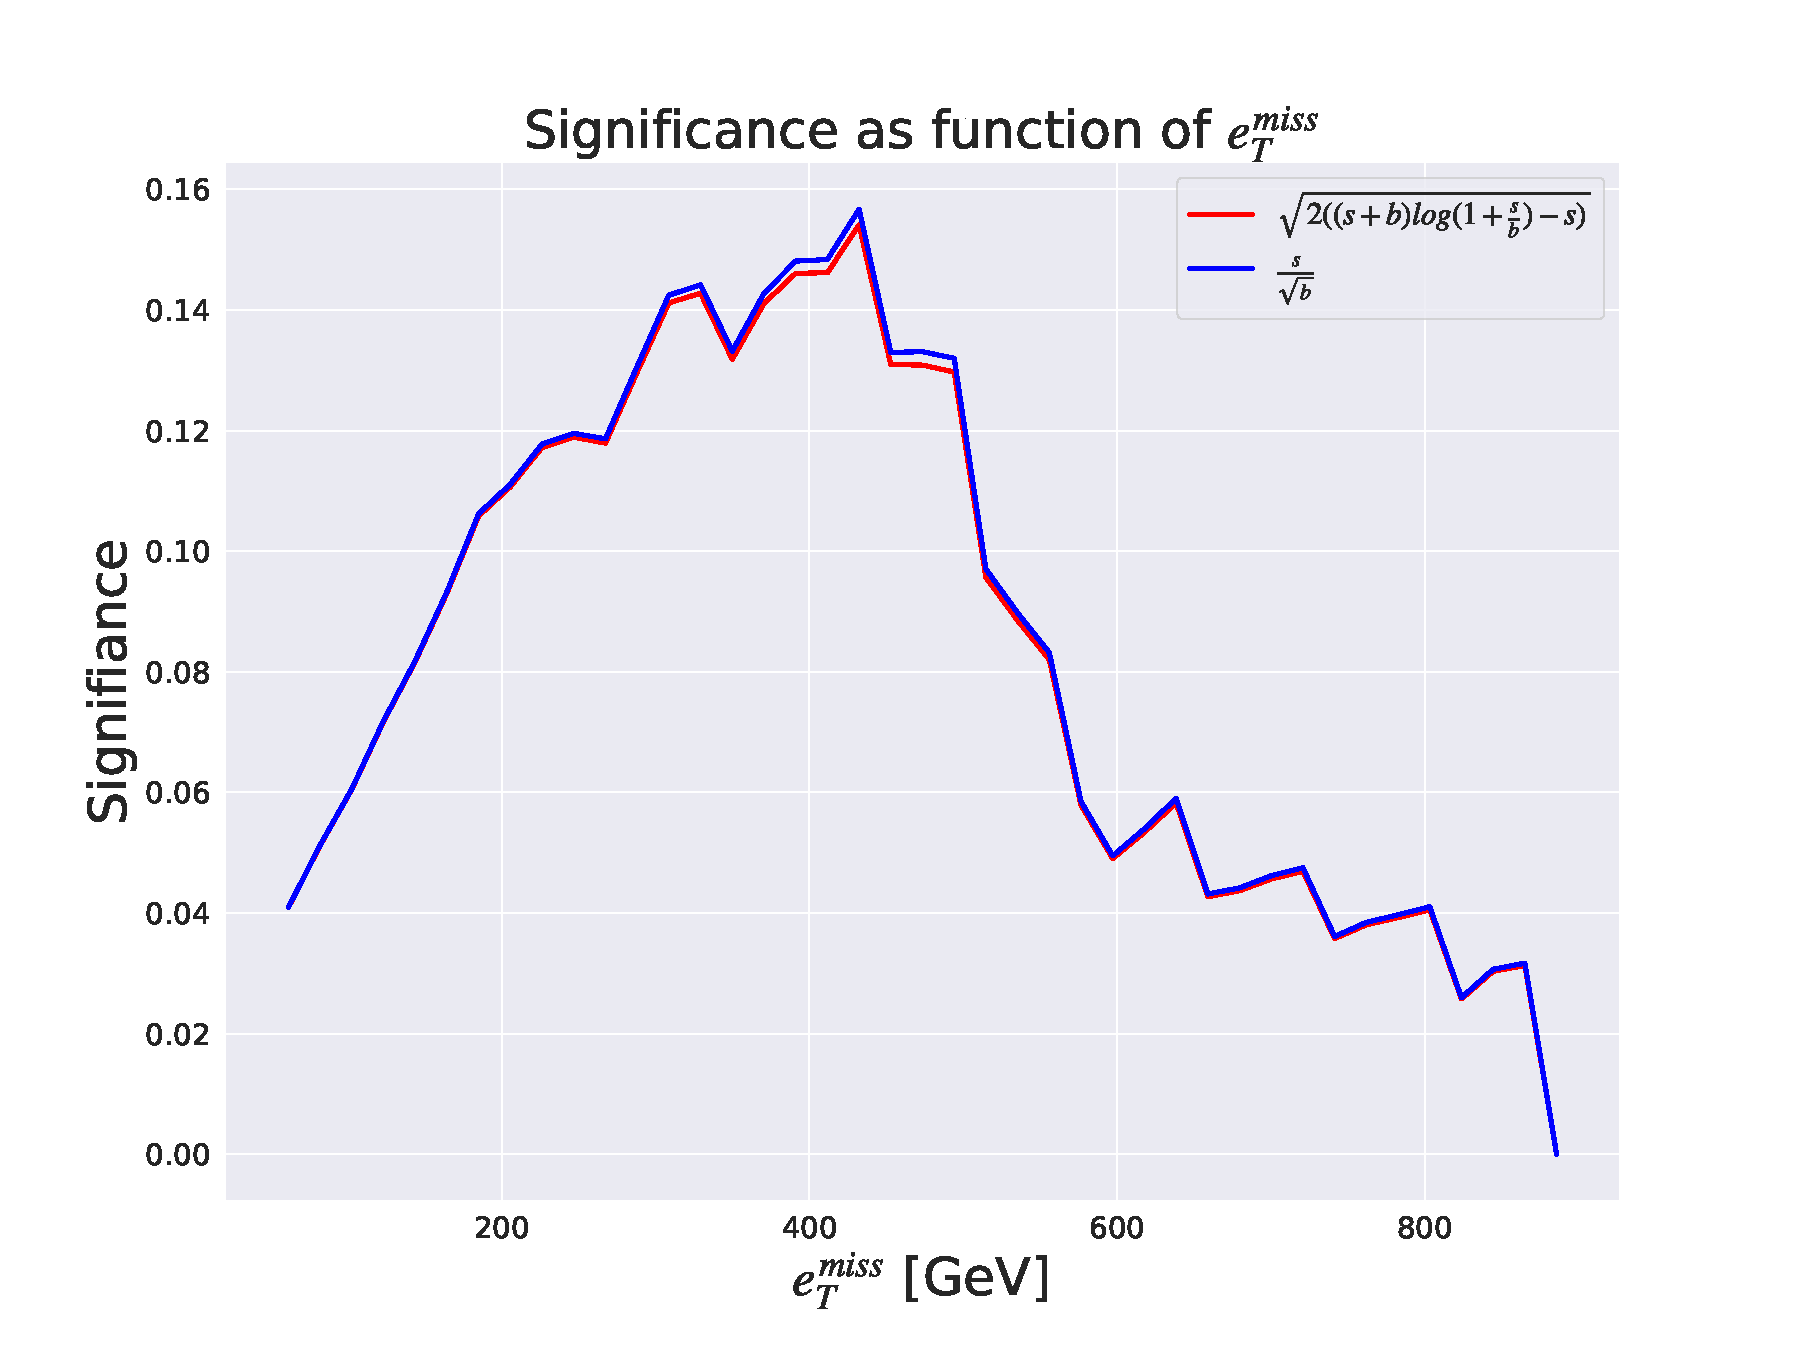
\includegraphics[width=\textwidth]{Figures/AE_testing/small/3lep/significance_etmiss_450p0p0300_-0.8533980148308666.pdf}
        \caption{}
        \label{fig:AE_3lep_small_signi_450_3}
    \end{subfigure}
    \hfill      
    \caption[3lep shallow network | $450p300$ | AE | 3]{Reconstruction error, $e_T^{miss}$ signal region, $m_{lll}$ signal region and significance as function of 
    $e_T^{miss}$ for the shallow regular autoencoder. Here the SUSY $450p300$ model is used. 
    Figure \ref{fig:AE_3lep_small_450_3} shows the reconstruction error 
    distribution for the SM MC and the SUSY signal. Here the autoencoder produce the same reconstruction error shape for both background and 
    signal. Figure \ref{fig:AE_3lep_small_etmiss_450_3} shows the $e_T^{miss}$ distribution for the SM MC and the SUSY signal in the signal region. 
    The signal region is made using a cut around $10^{-0.85}$. Most of the background is removed, with almost no signal in the signal region.
    Figure \ref{fig:AE_3lep_small_mlll_450_3} shows the $m_{lll}$ distribution for the SM MC and the SUSY signal. 
    There is almost no signal in the signal region. Figure \ref{fig:AE_3lep_small_signi_450_3} shows the significance as function of
    $e_T^{miss}$. The peak is put around a cut of about 430 GeV in the $e_T^{miss}$, with a significance of around $0.155$.}
    \label{fig:AE_3lep_small_rec_sig_signi_450_3}
\end{figure}








\begin{figure}[H]
    \centering
    \begin{subfigure}{.40\textwidth}
        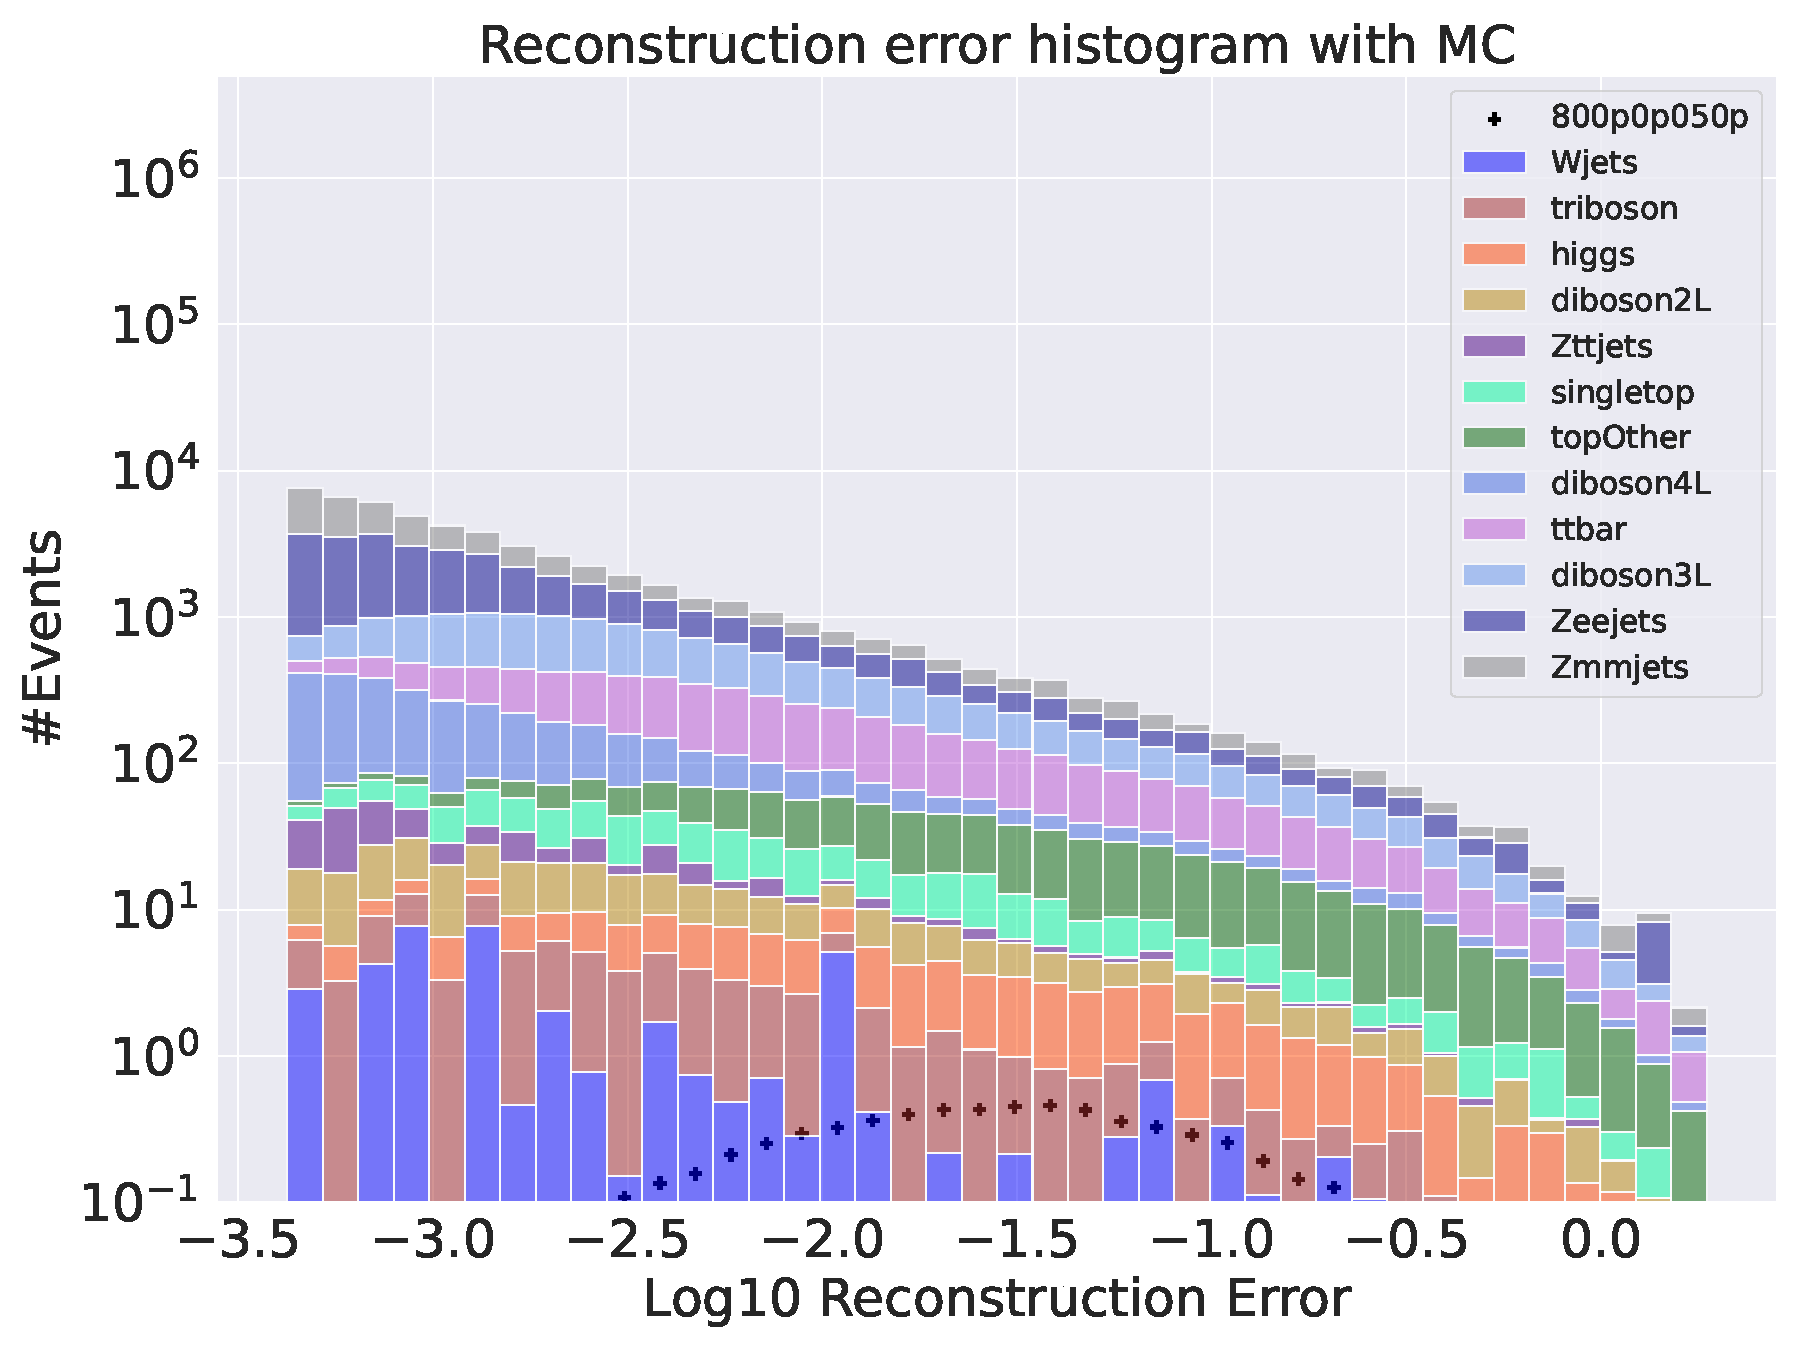
\includegraphics[width=\textwidth]{Figures/AE_testing/big/3lep/b_data_recon_big_rm3_feats_sig_800p0p050p.pdf}
        \caption{ }
        \label{fig:AE_3lep_big_800_3}
    \end{subfigure}
    \hfill
    \begin{subfigure}{.40\textwidth}
        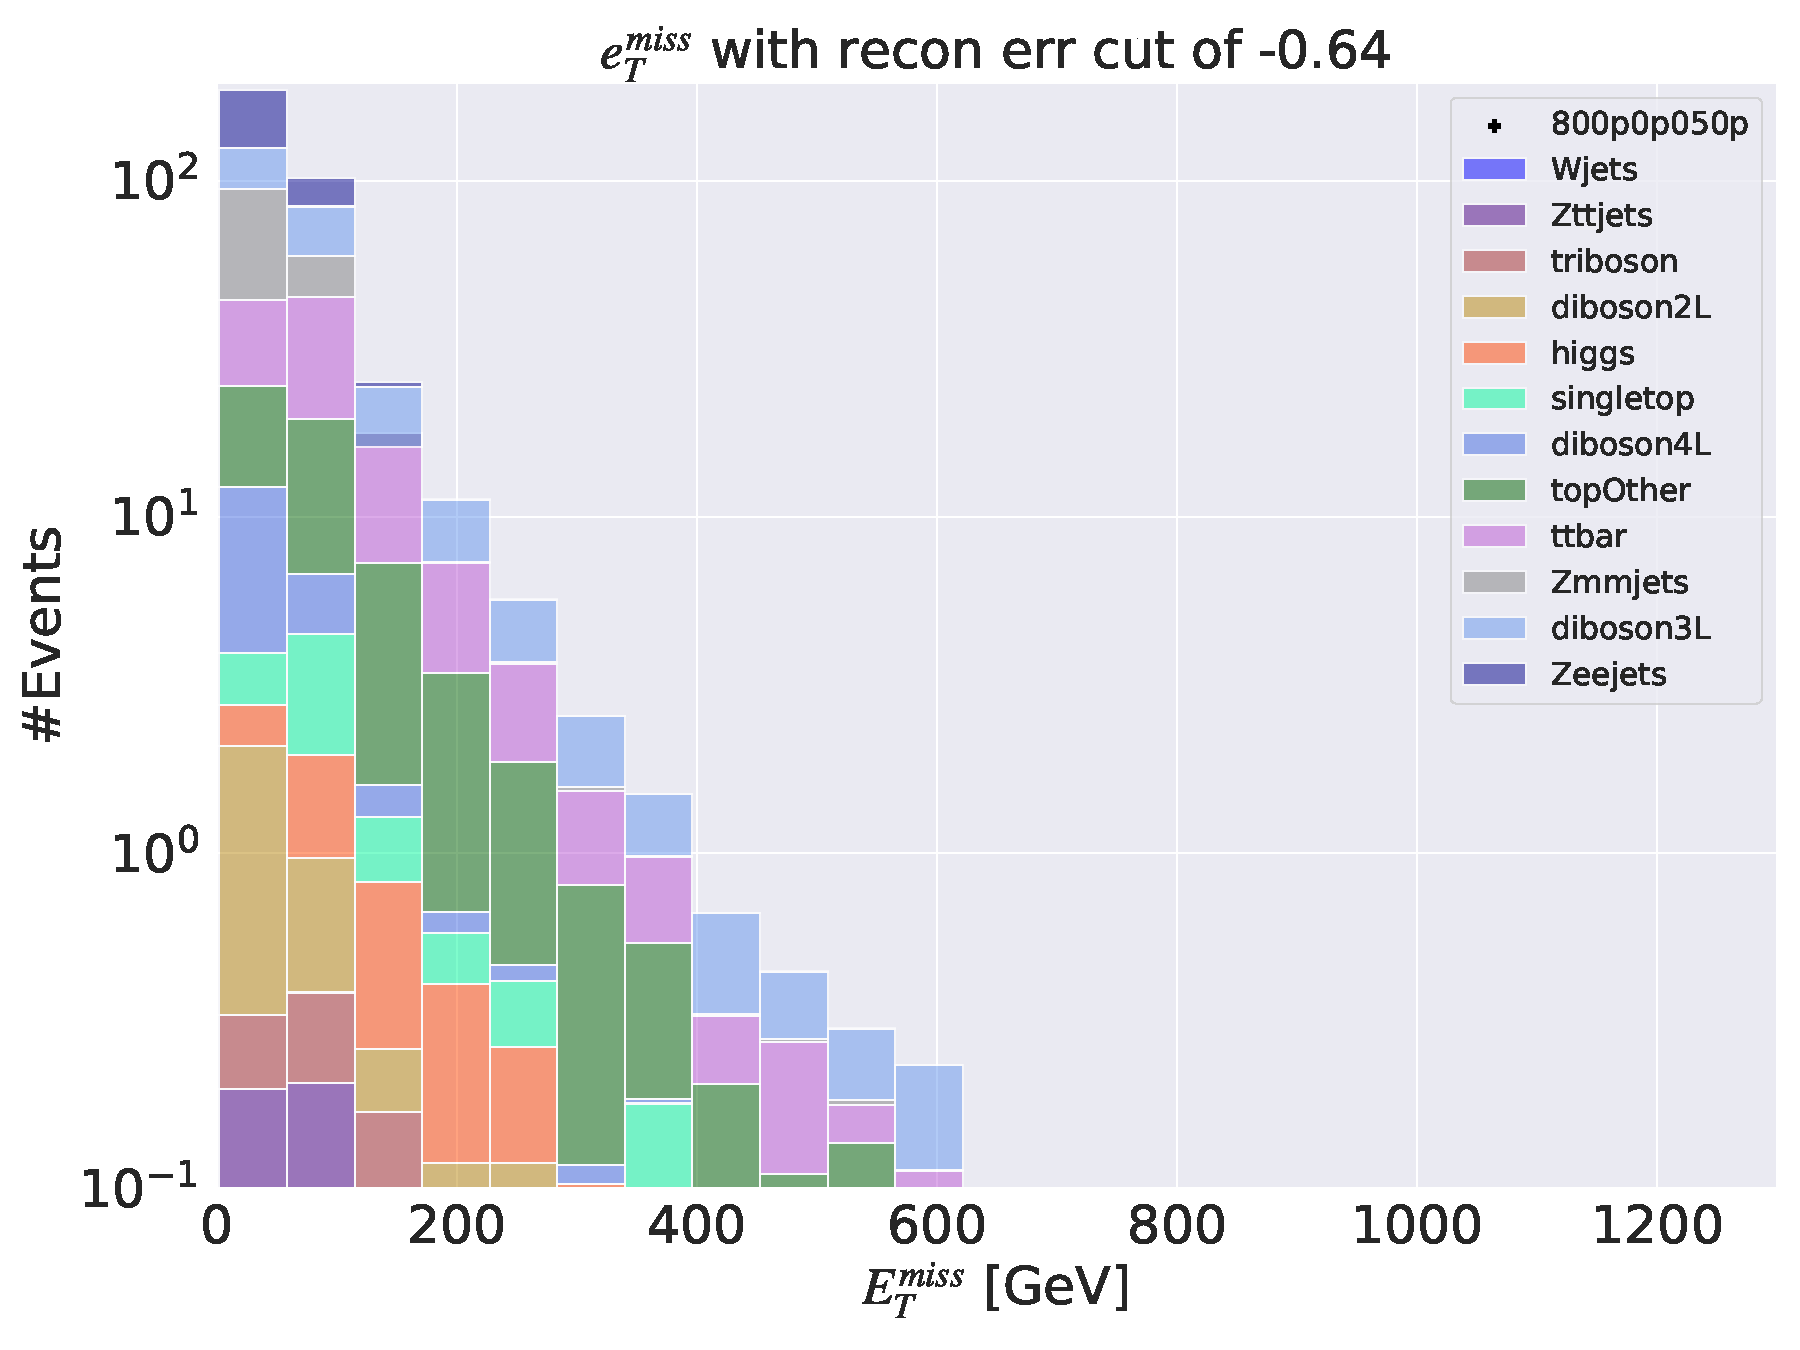
\includegraphics[width=\textwidth]{Figures/AE_testing/big/3lep/b_data_recon_big_rm3_feats_sig_800p0p050p_etmiss_recon_errcut_-0.64.pdf}
        \caption{}
        \label{fig:AE_3lep_big_etmiss_800_3}
    \end{subfigure}
    \hfill
    \begin{subfigure}{.40\textwidth}
        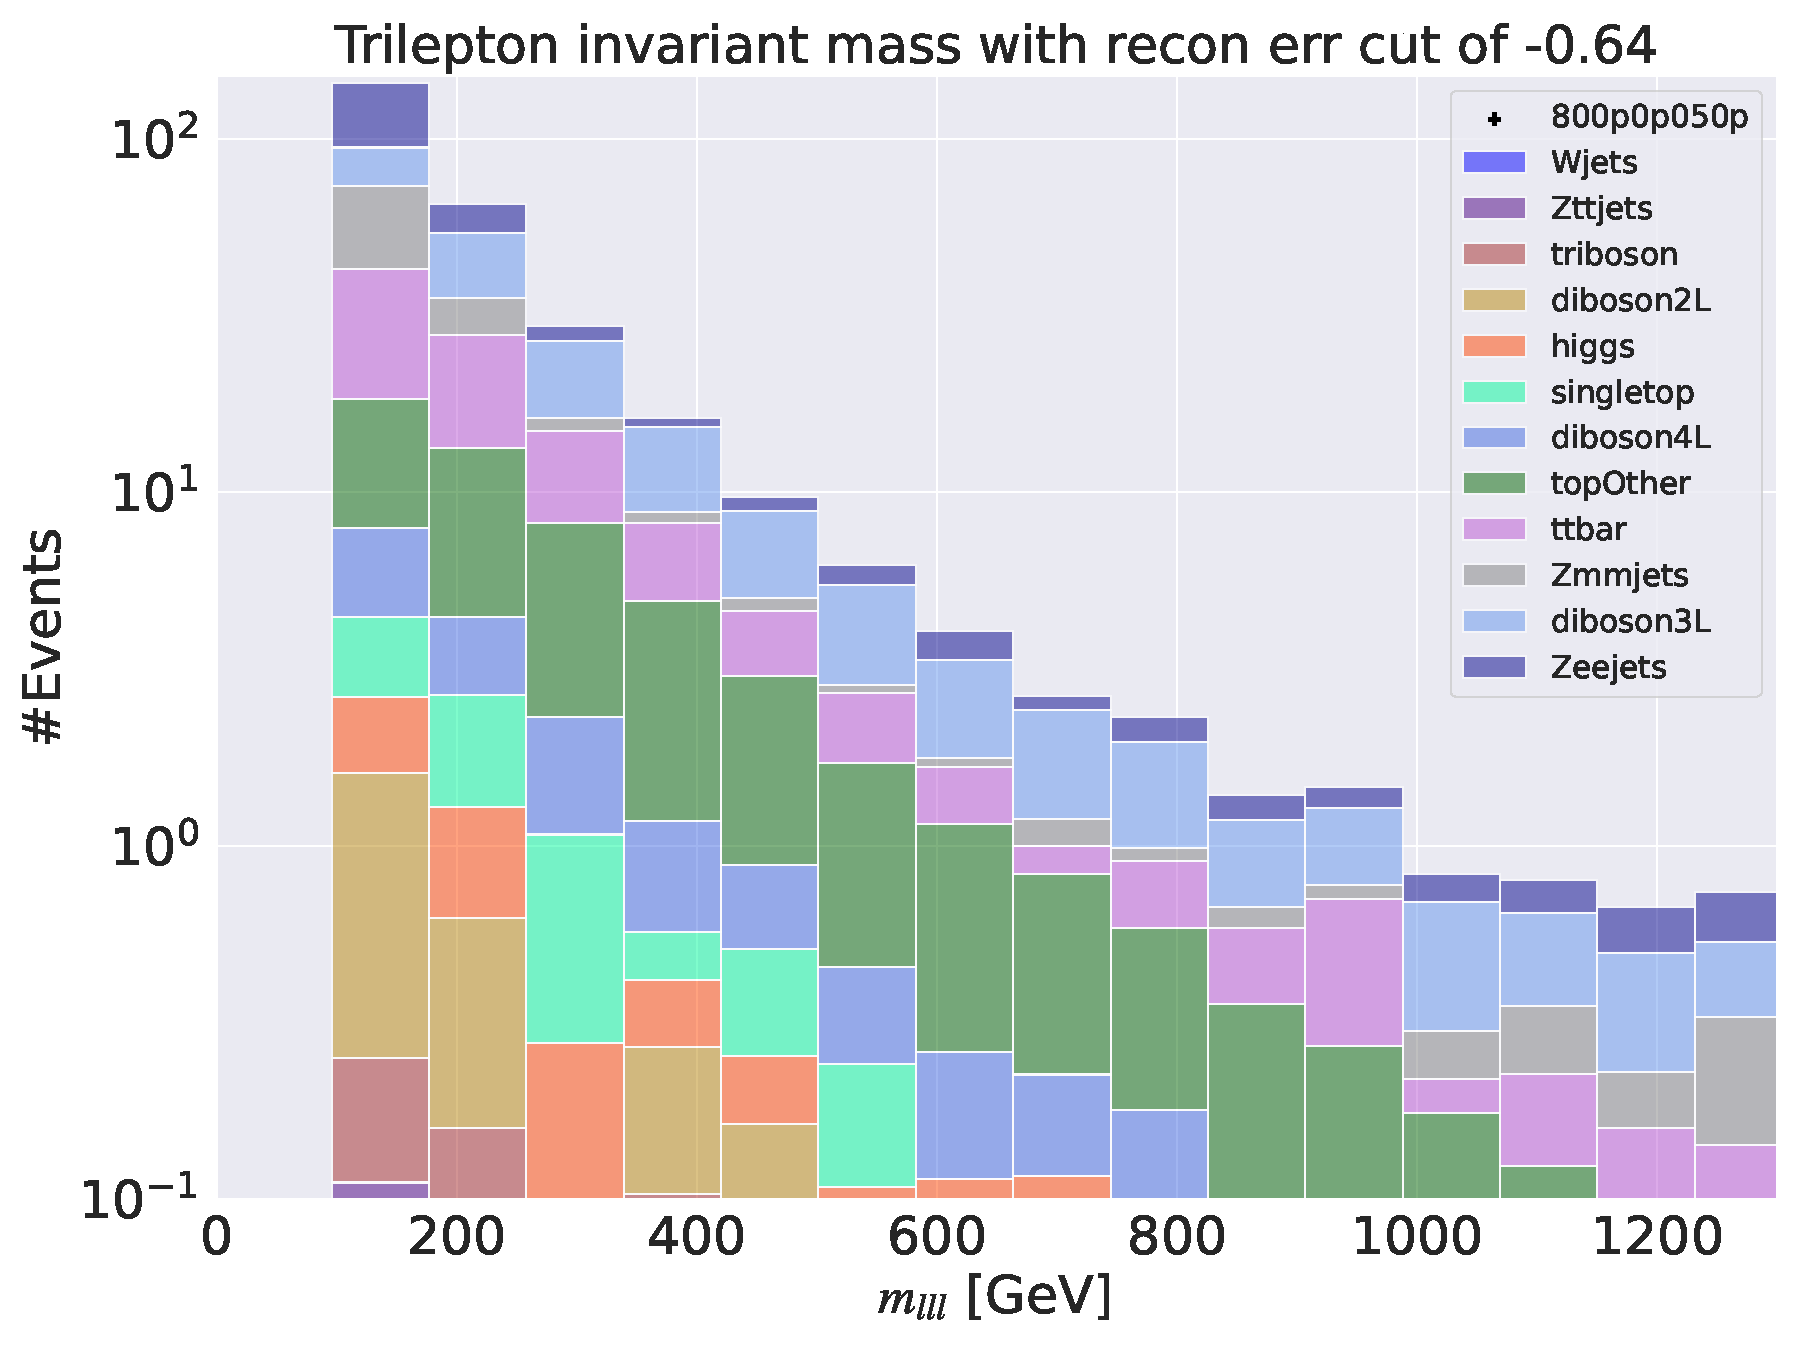
\includegraphics[width=\textwidth]{Figures/AE_testing/big/3lep/b_data_recon_big_rm3_feats_sig_800p0p050p_mlll_recon_errcut_-0.64.pdf}
        \caption{}
        \label{fig:AE_3lep_big_mlll_800_3}
    \end{subfigure}
    \hfill   
    \begin{subfigure}{.40\textwidth}
        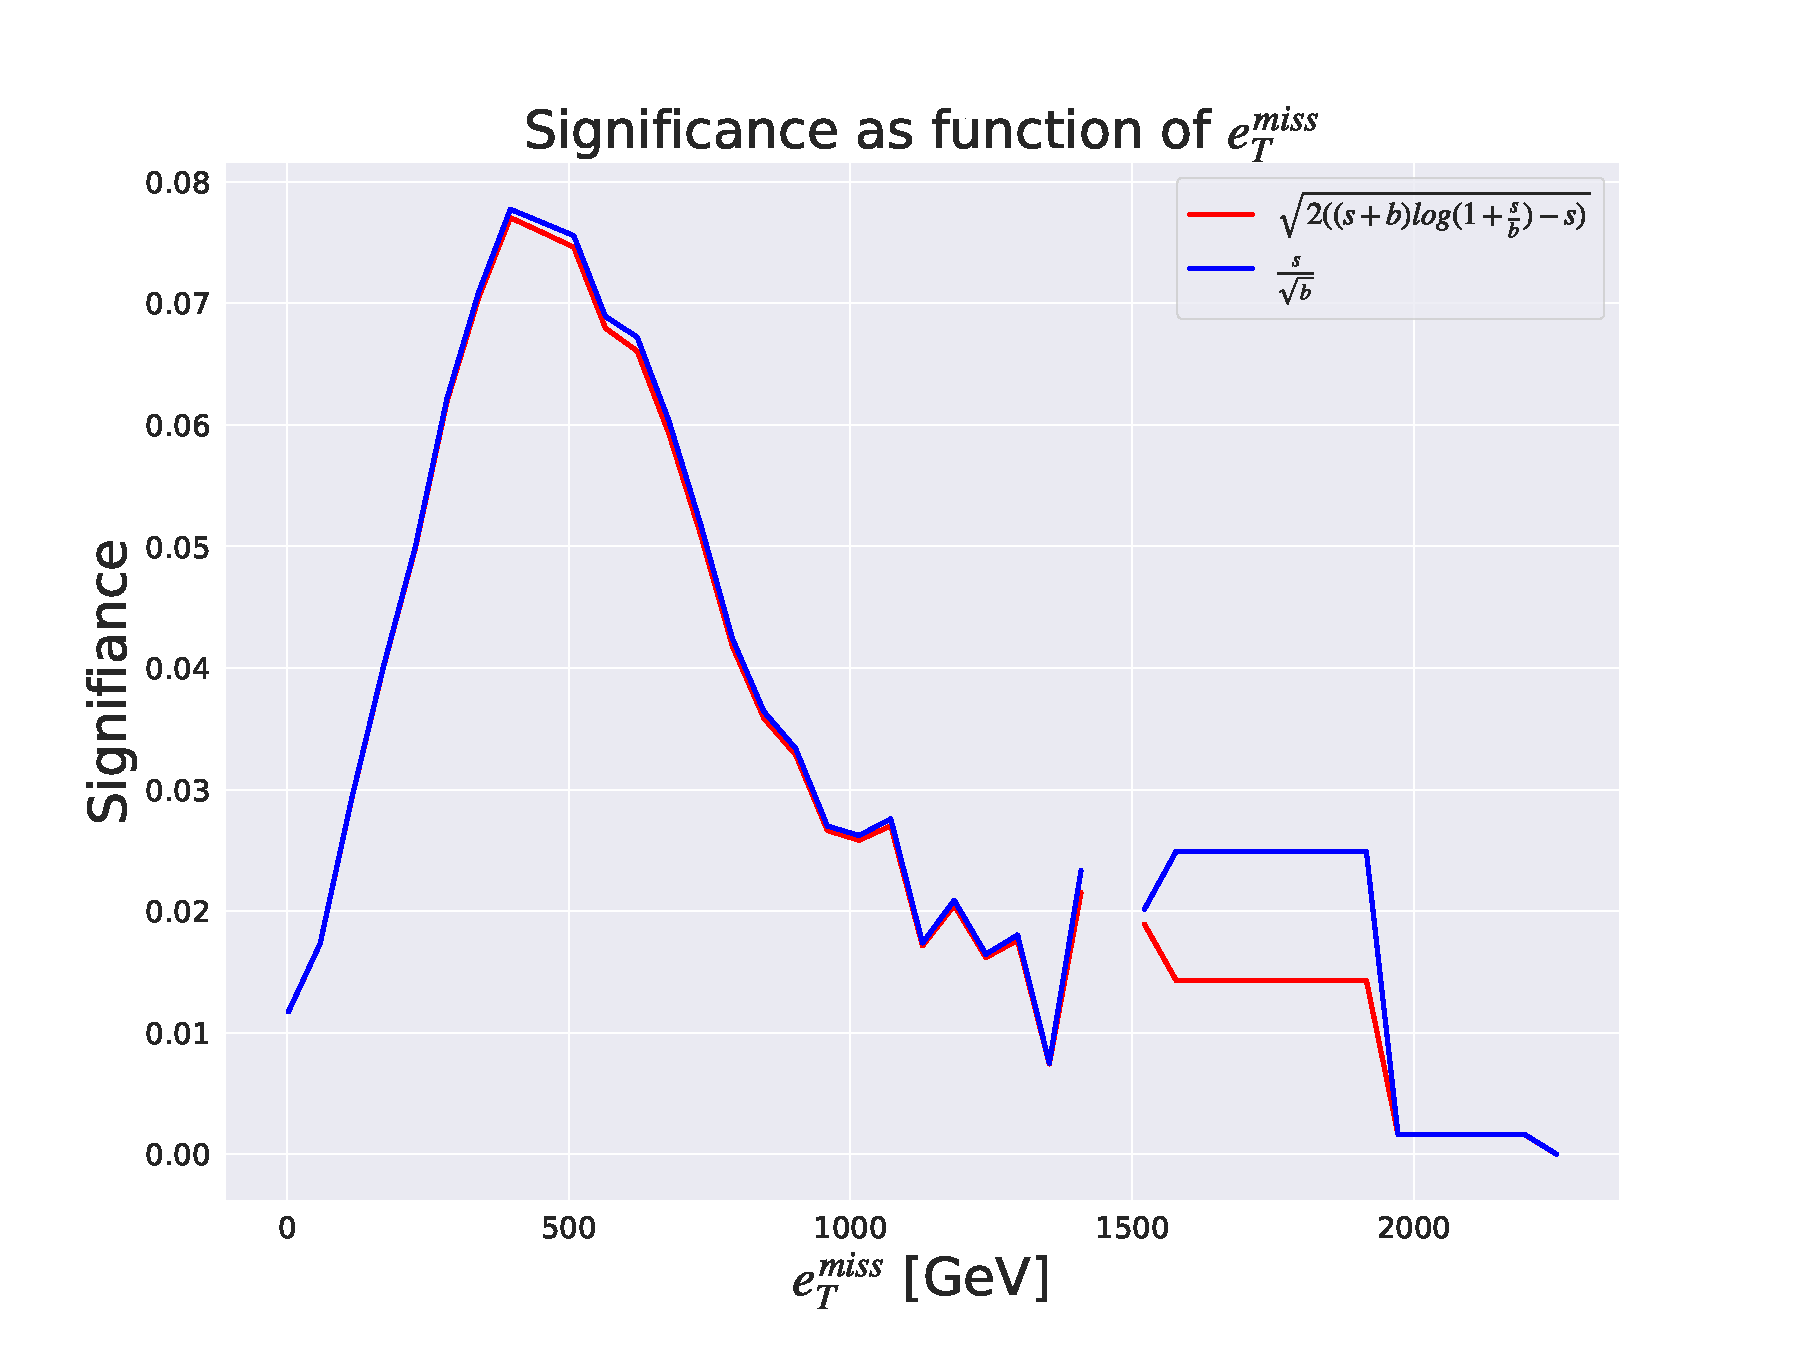
\includegraphics[width=\textwidth]{Figures/AE_testing/big/3lep/significance_etmiss_800p0p050p_-0.6363296281507171.pdf}
        \caption{}
        \label{fig:AE_3lep_big_signi_800_3}
    \end{subfigure}
    \hfill      
    \caption[3lep deep network | $800p50$ | AE | 3]{Reconstruction error, $e_T^{miss}$ signal region, $m_{lll}$ signal region and significance as function of 
    $e_T^{miss}$ for the deep regular autoencoder. Here the SUSY $450p300$ model is used.
    Figure \ref{fig:AE_3lep_big_800_3} shows the reconstruction error 
    distribution for the SM MC and the SUSY signal. Here the autoencoder produce a mirrored reconstruction error shape for both background and 
    signal. Figure \ref{fig:AE_3lep_big_etmiss_800_3} shows the $e_T^{miss}$ distribution for the SM MC and the SUSY signal in the signal region. 
    The signal region is made using a cut around $10^{-0.64}$. Most of the background is removed, with almost no signal in the signal region.
    Figure \ref{fig:AE_3lep_big_mlll_800_3} shows the $m_{lll}$ distribution for the SM MC and the SUSY signal. 
    There is almost no signal in the signal region. Figure \ref{fig:AE_3lep_big_signi_800_3} shows the significance as function of
    $e_T^{miss}$. The peak is put around a cut of about 400 GeV in the $e_T^{miss}$, with a significance of around $0.078$.}
    \label{fig:AE_3lep_big_rec_sig_signi_800_3}
\end{figure}

\begin{figure}[H]
    \centering
    \begin{subfigure}{.40\textwidth}
        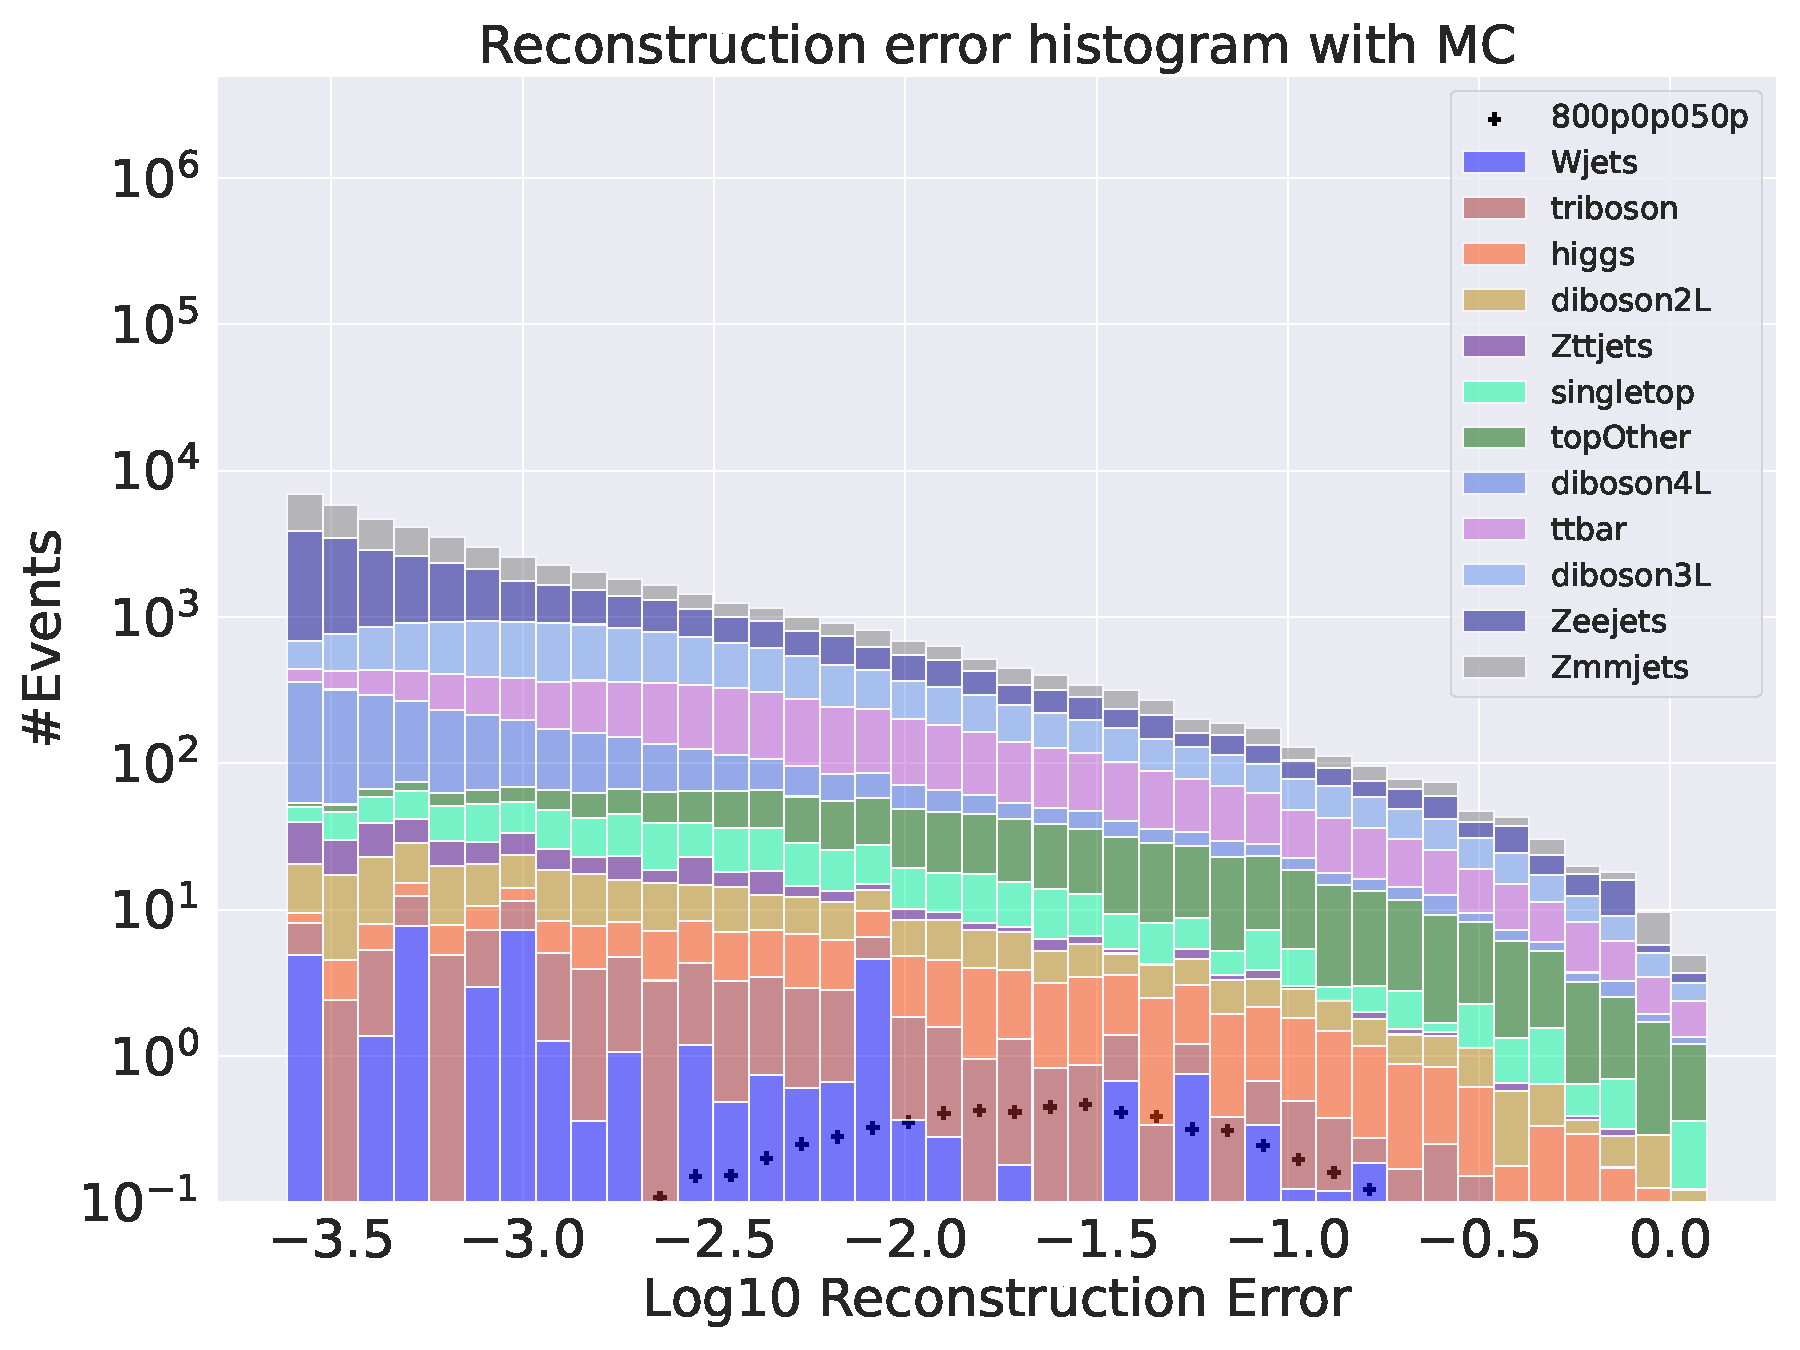
\includegraphics[width=\textwidth]{Figures/AE_testing/small/3lep/b_data_recon_big_rm3_feats_sig_800p0p050p.pdf}
        \caption{ }
        \label{fig:AE_3lep_small_800_3}
    \end{subfigure}
    \hfill
    \begin{subfigure}{.40\textwidth}
        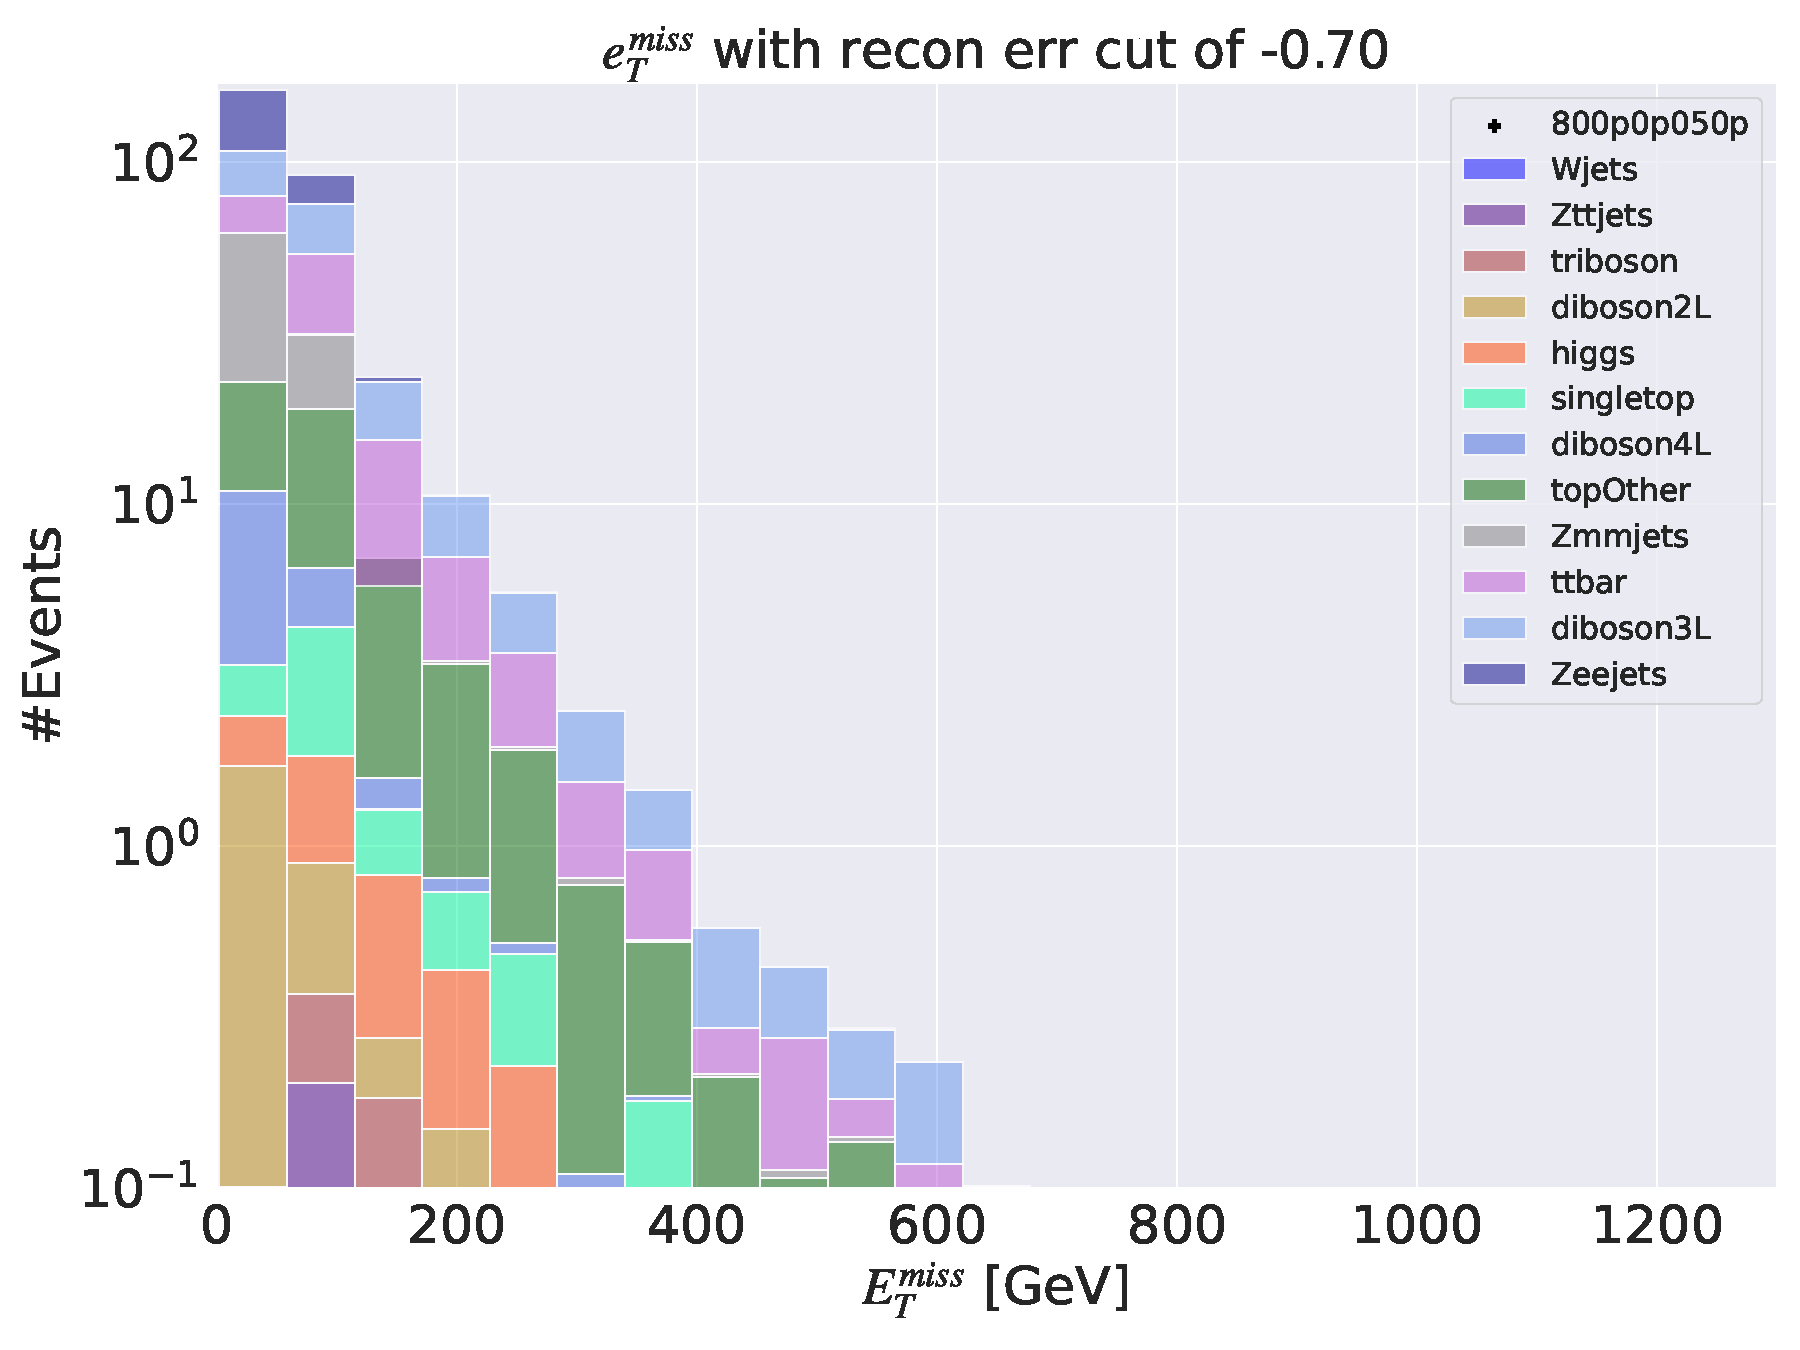
\includegraphics[width=\textwidth]{Figures/AE_testing/small/3lep/b_data_recon_big_rm3_feats_sig_800p0p050p_etmiss_recon_errcut_-0.70.pdf}
        \caption{}
        \label{fig:AE_3lep_small_etmiss_800_3}
    \end{subfigure}
    \hfill
    \begin{subfigure}{.40\textwidth}
        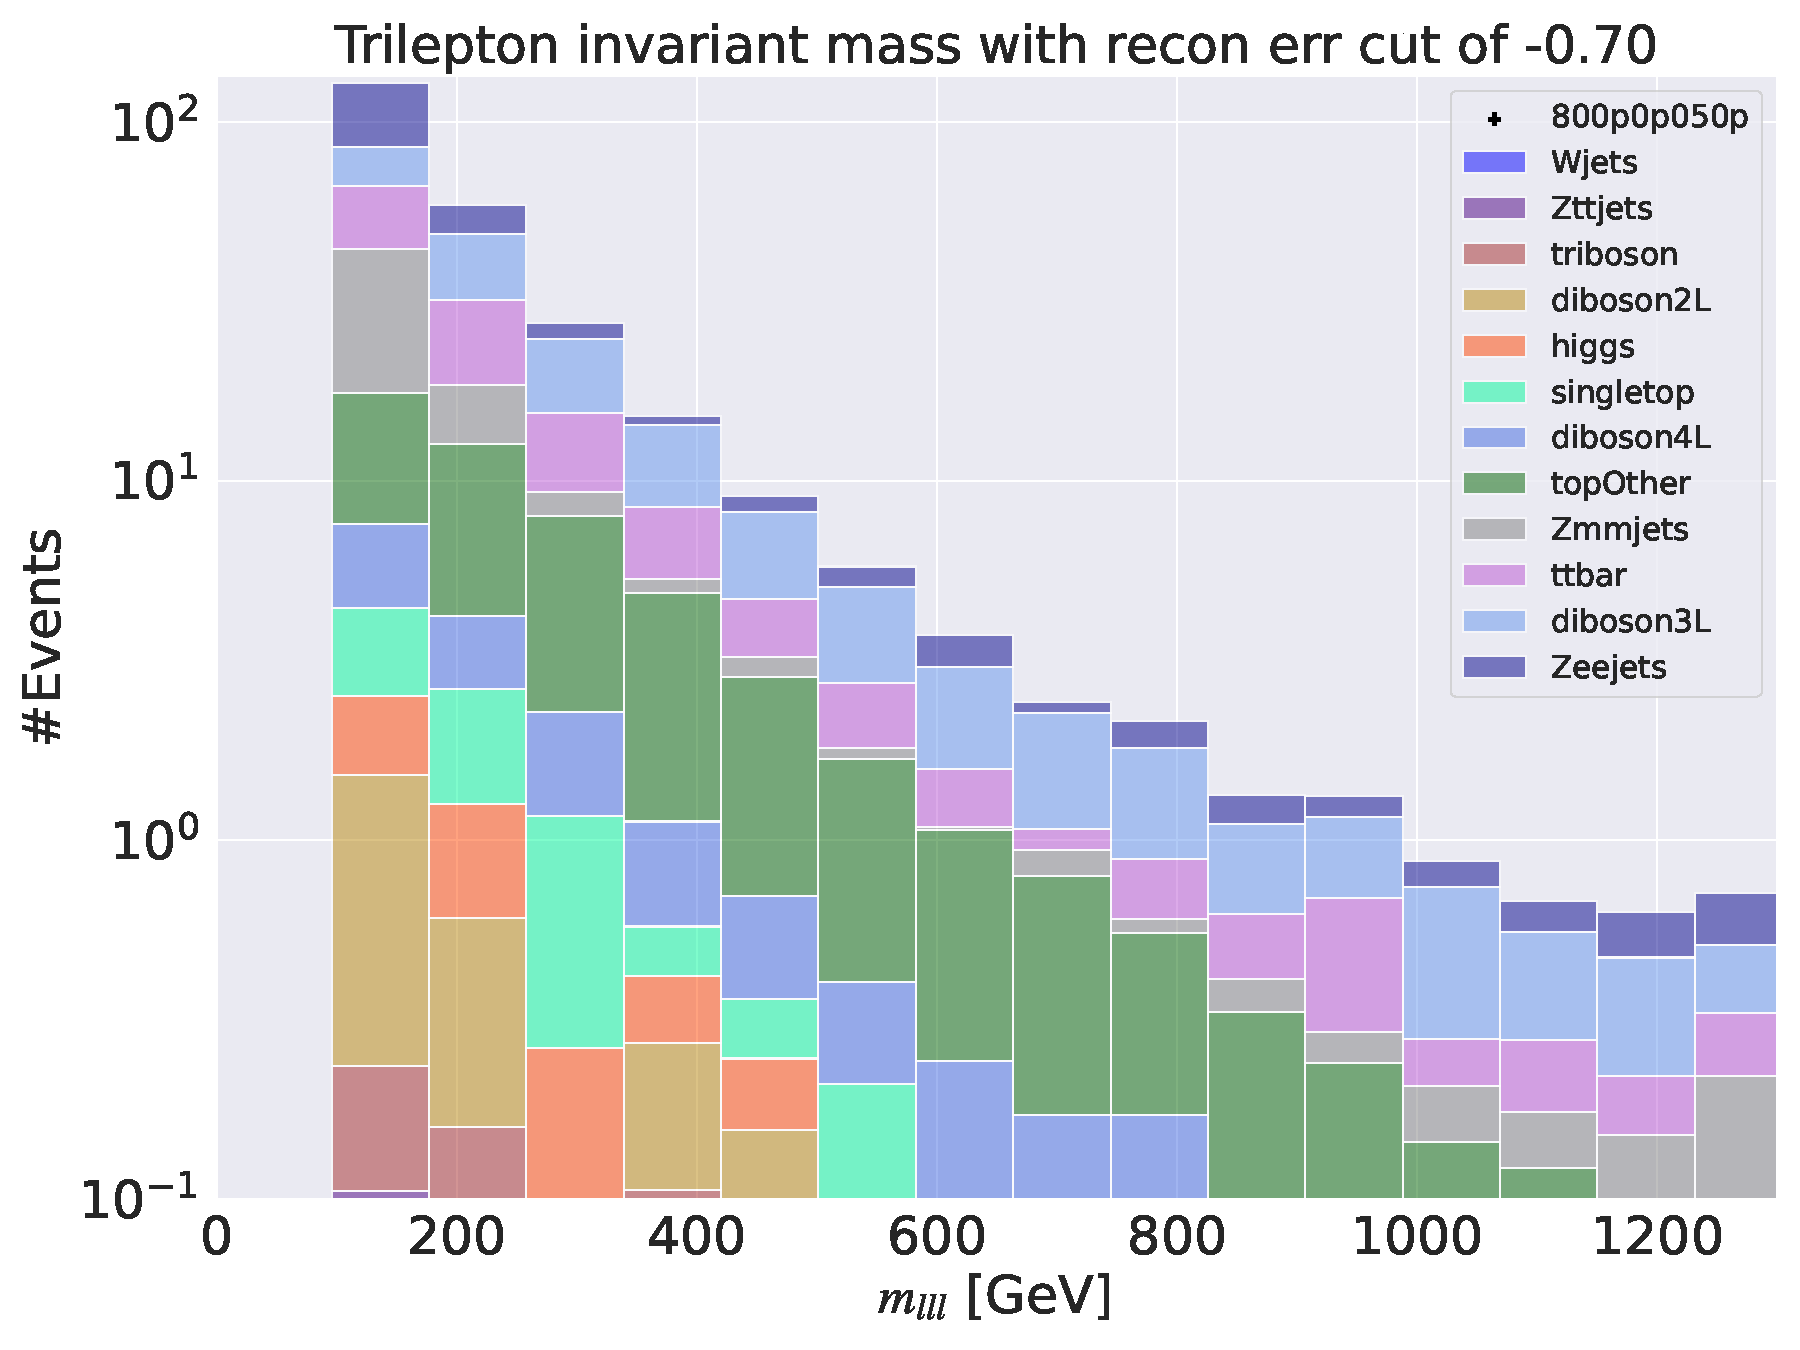
\includegraphics[width=\textwidth]{Figures/AE_testing/small/3lep/b_data_recon_big_rm3_feats_sig_800p0p050p_mlll_recon_errcut_-0.70.pdf}
        \caption{}
        \label{fig:AE_3lep_small_mlll_800_3}
    \end{subfigure}
    \hfill   
    \begin{subfigure}{.40\textwidth}
        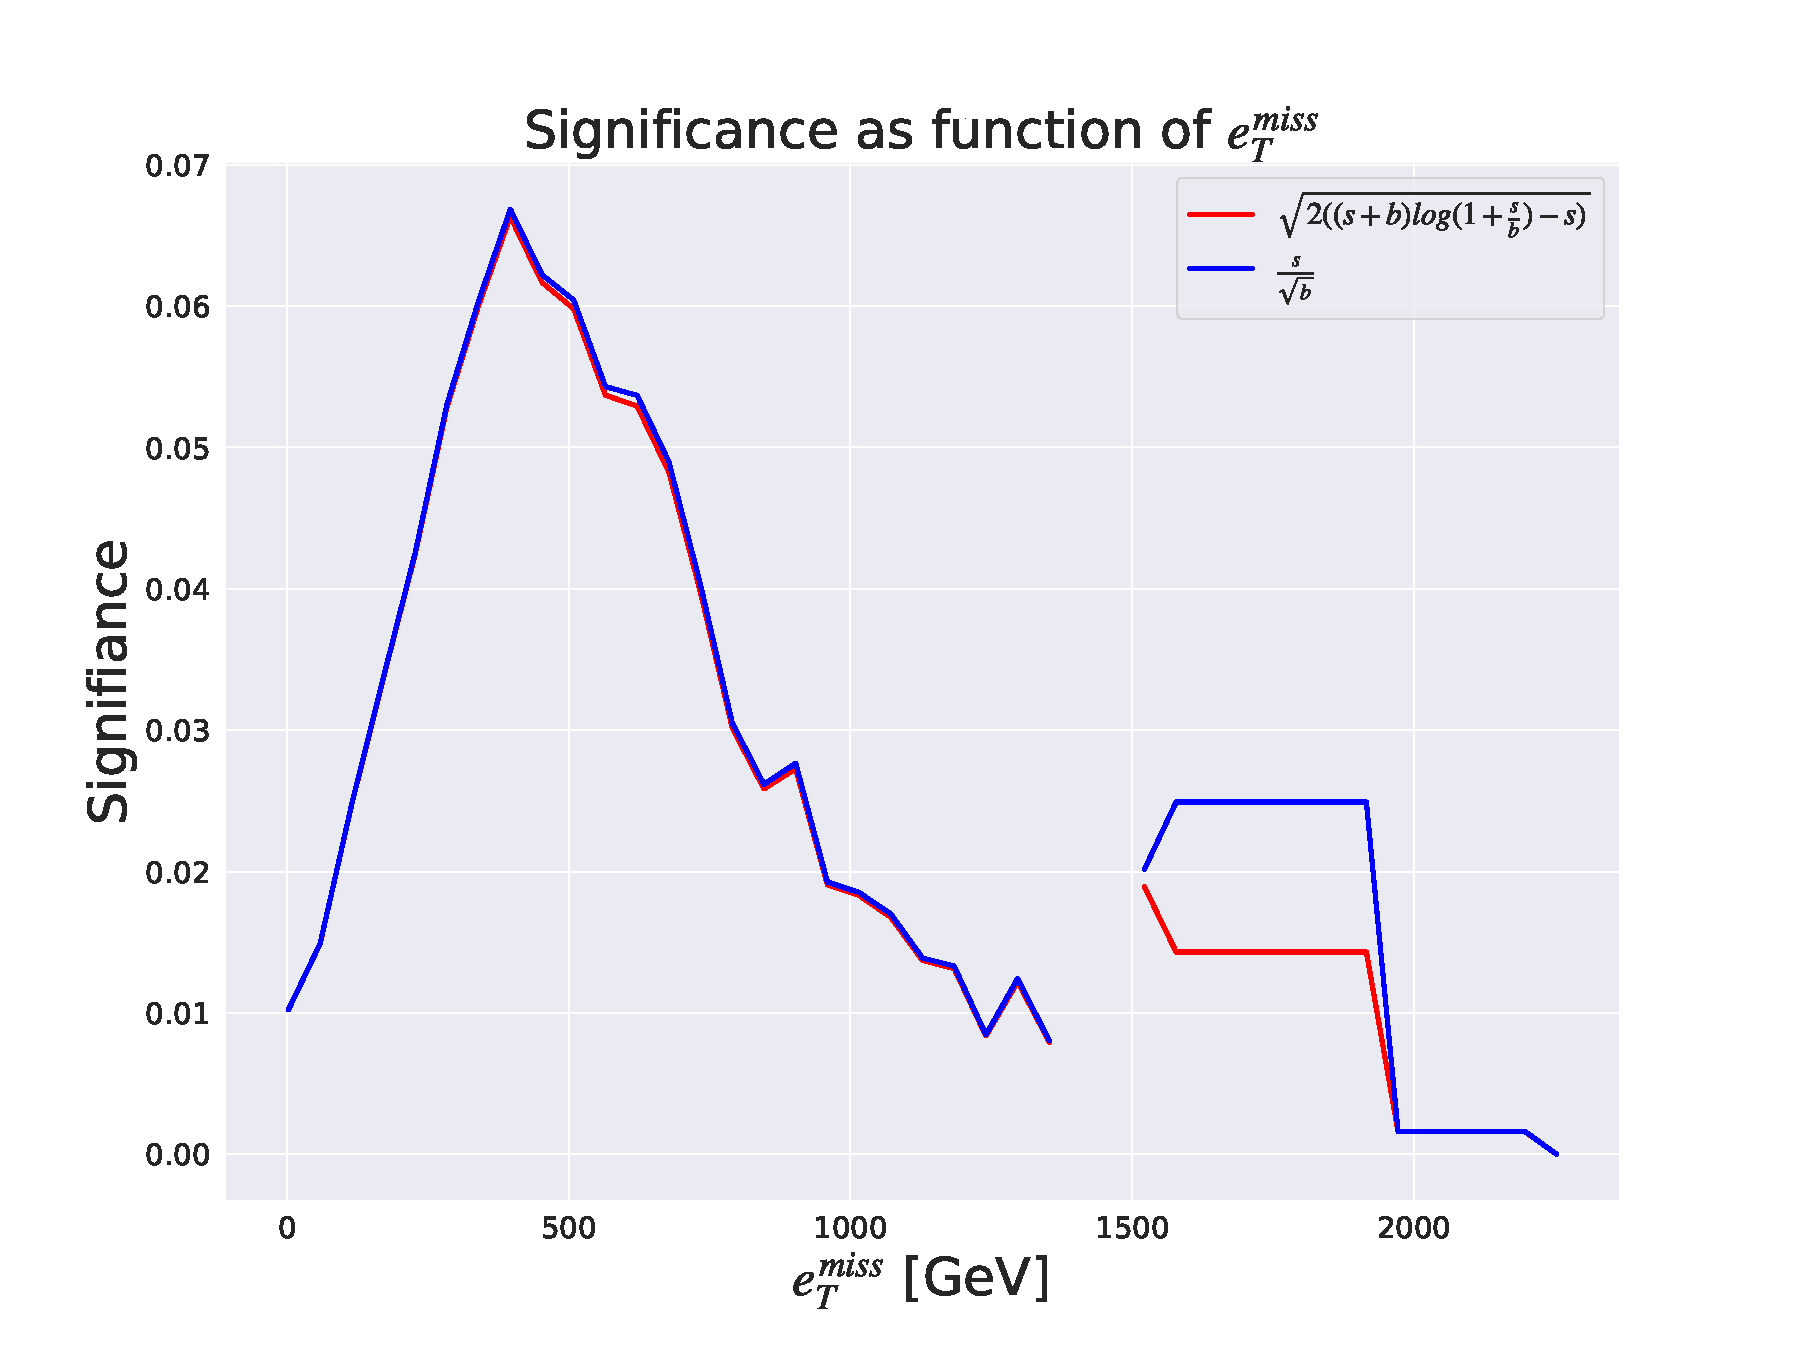
\includegraphics[width=\textwidth]{Figures/AE_testing/small/3lep/significance_etmiss_800p0p050p_-0.7044693201264449.pdf}
        \caption{}
        \label{fig:AE_3lep_small_signi_800_3}
    \end{subfigure}
    \hfill      
    \caption[3lep shallow network | $800p50$ | AE | 3]{Reconstruction error, $e_T^{miss}$ signal region, $m_{lll}$ signal region and significance as function of 
    $e_T^{miss}$ for the shallow regular autoencoder. Here the SUSY $450p300$ model is used.
    Figure \ref{fig:AE_3lep_small_800_3} shows the reconstruction error 
    distribution for the SM MC and the SUSY signal. Here the autoencoder produce a mirrored reconstruction error shape for both background and 
    signal. Figure \ref{fig:AE_3lep_small_etmiss_800_3} shows the $e_T^{miss}$ distribution for the SM MC and the SUSY signal in the signal region. 
    The signal region is made using a cut around $10^{-0.95}$. Most of the background is removed, with almost no signal in the signal region.
    Figure \ref{fig:AE_3lep_small_mlll_800_3} shows the $m_{lll}$ distribution for the SM MC and the SUSY signal. 
    There is almost no signal in the signal region. Figure \ref{fig:AE_3lep_small_signi_800_3} shows the significance as function of
    $e_T^{miss}$. The peak is put around a cut of about 400 GeV in the $e_T^{miss}$, with a significance of around $0.067$.}
    \label{fig:AE_3lep_small_rec_sig_signi_800_3}
\end{figure}










\subsection*{Variational autoencoder output}












\begin{figure}[H]
    \centering
    \begin{subfigure}{.40\textwidth}
        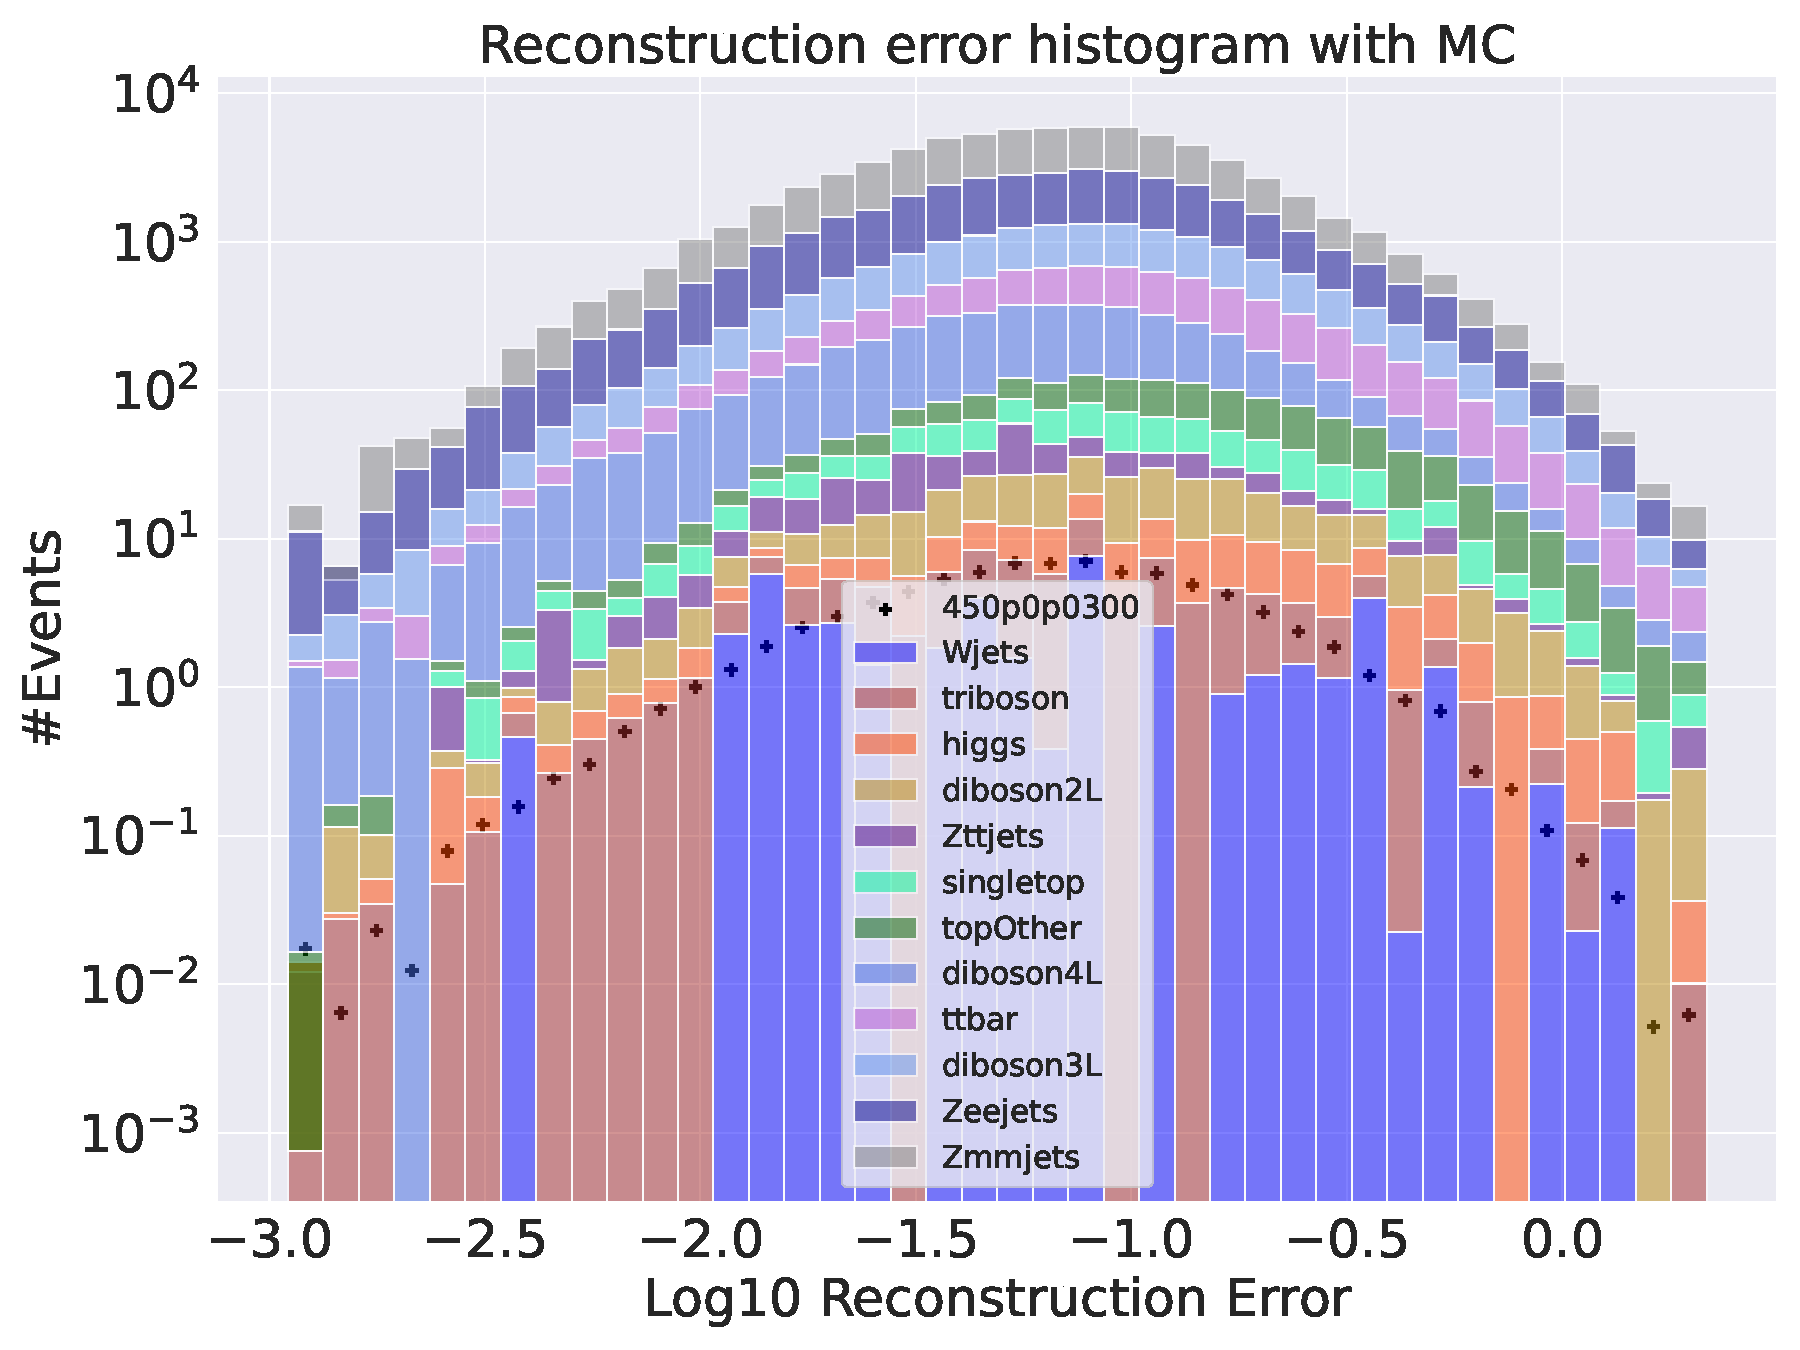
\includegraphics[width=\textwidth]{Figures/VAE_testing/big/3lep/b_data_recon_big_rm3_feats_sig_450p0p0300.pdf}
        \caption{ }
        \label{fig:VAE_3lep_big_450_2}
    \end{subfigure}
    \hfill
    \begin{subfigure}{.40\textwidth}
        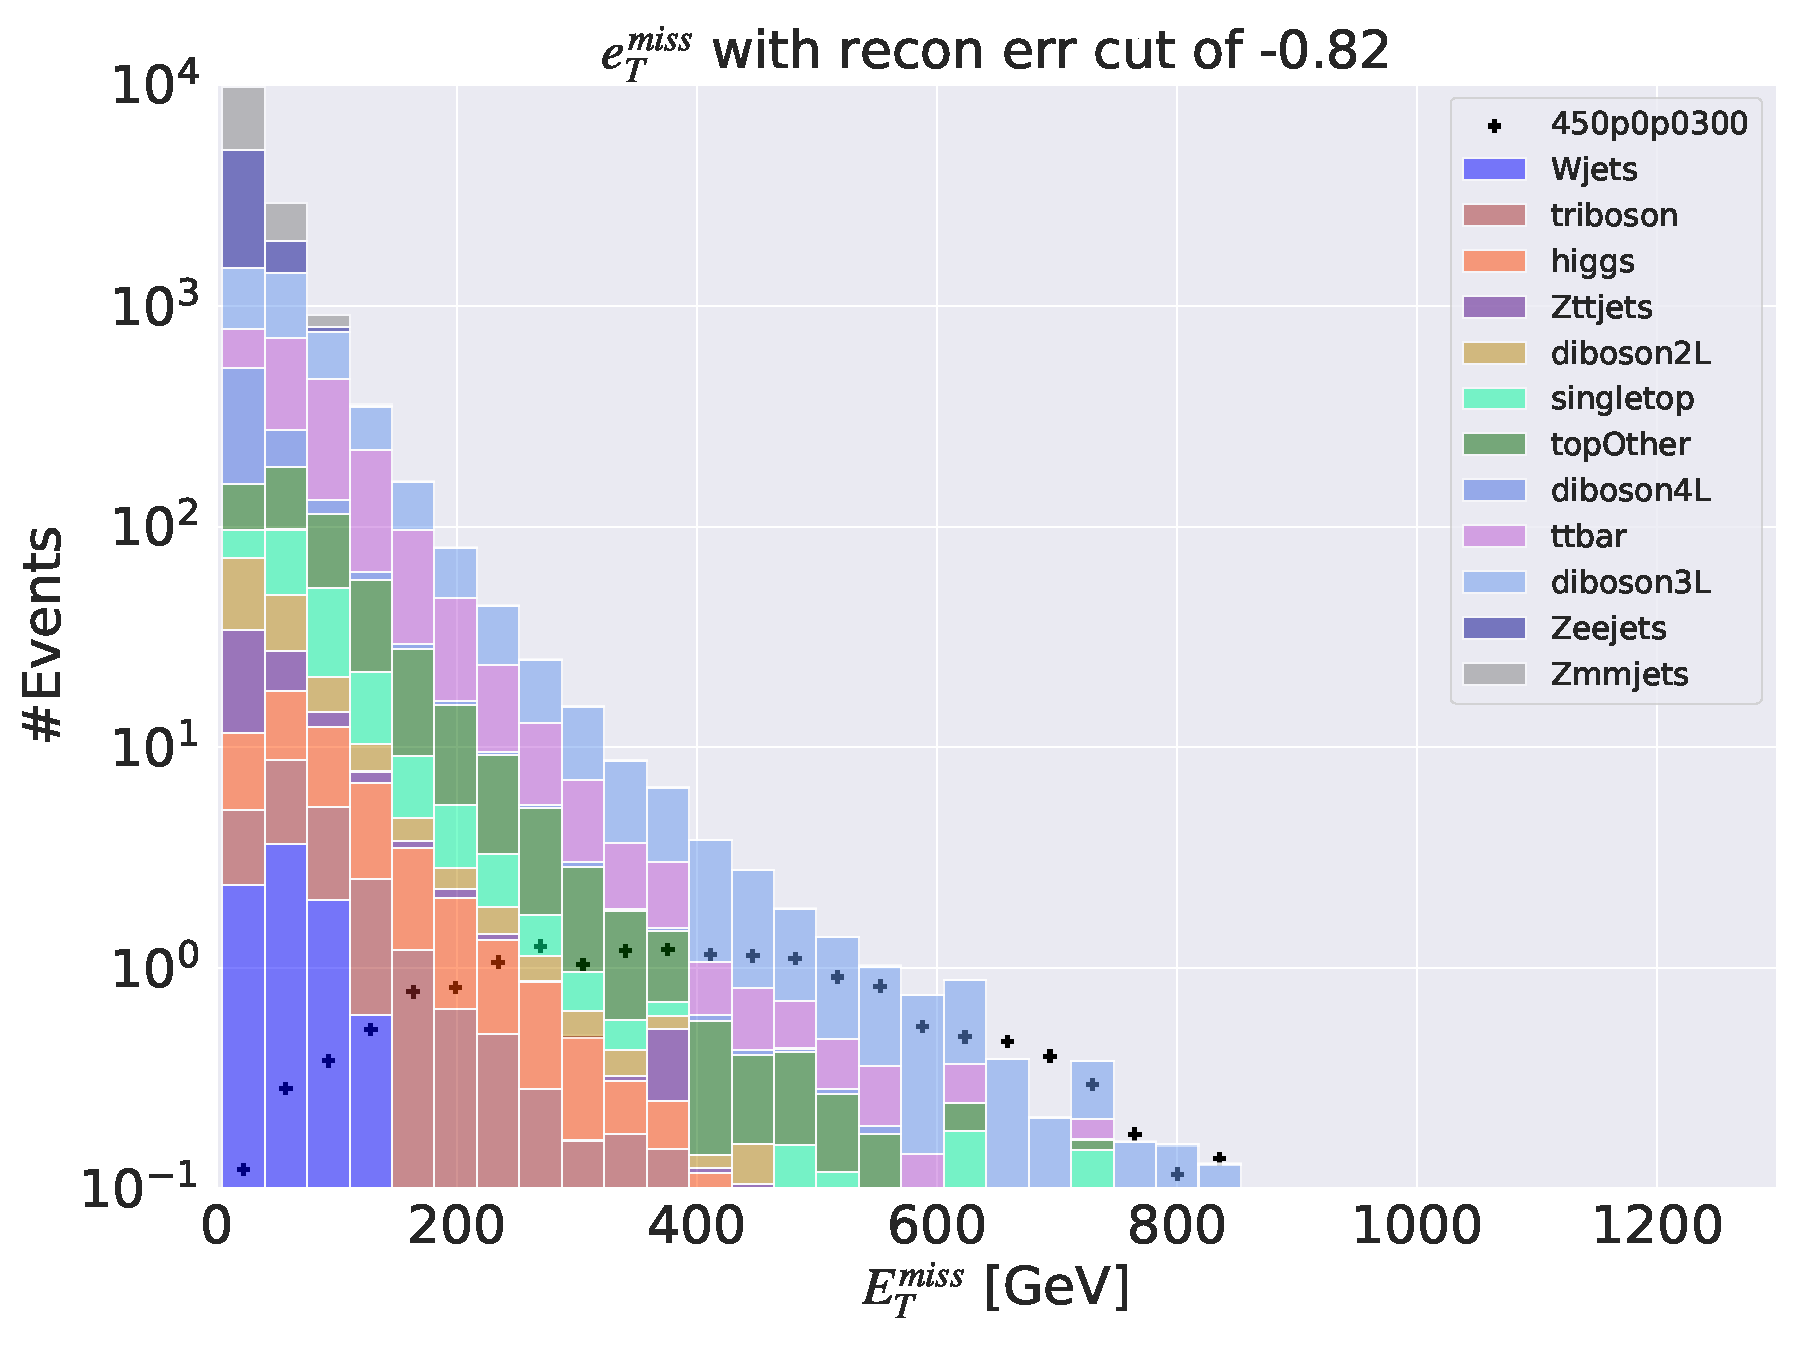
\includegraphics[width=\textwidth]{Figures/VAE_testing/big/3lep/b_data_recon_big_rm3_feats_sig_450p0p0300_etmiss_recon_errcut_-0.82.pdf}
        \caption{}
        \label{fig:VAE_3lep_big_etmiss_450_2}
    \end{subfigure}
    \hfill
    \begin{subfigure}{.40\textwidth}
        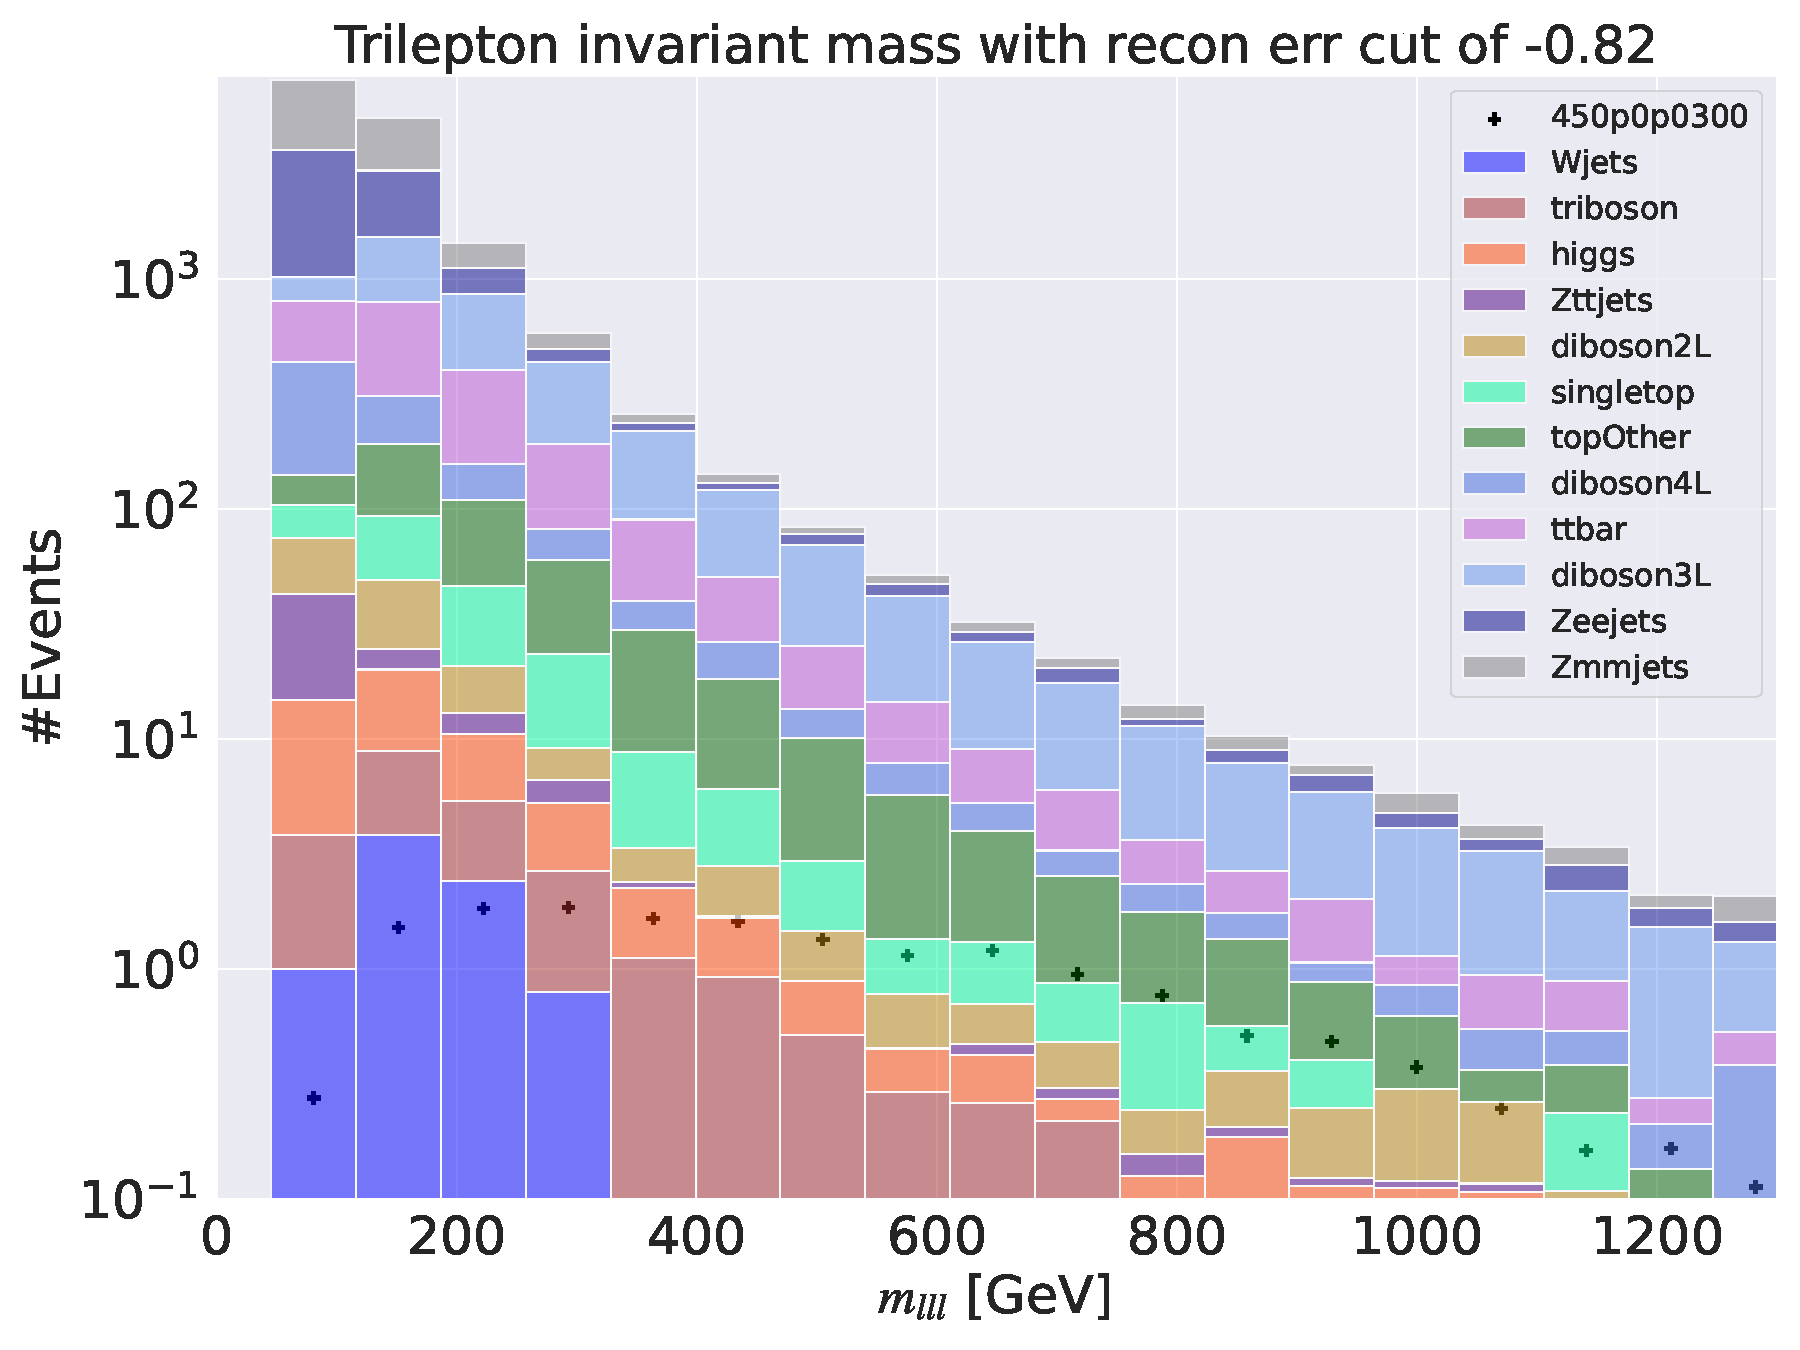
\includegraphics[width=\textwidth]{Figures/VAE_testing/big/3lep/b_data_recon_big_rm3_feats_sig_450p0p0300_mlll_recon_errcut_-0.82.pdf}
        \caption{}
        \label{fig:VAE_3lep_big_mlll_450_2}
    \end{subfigure}
    \hfill   
    \begin{subfigure}{.40\textwidth}
        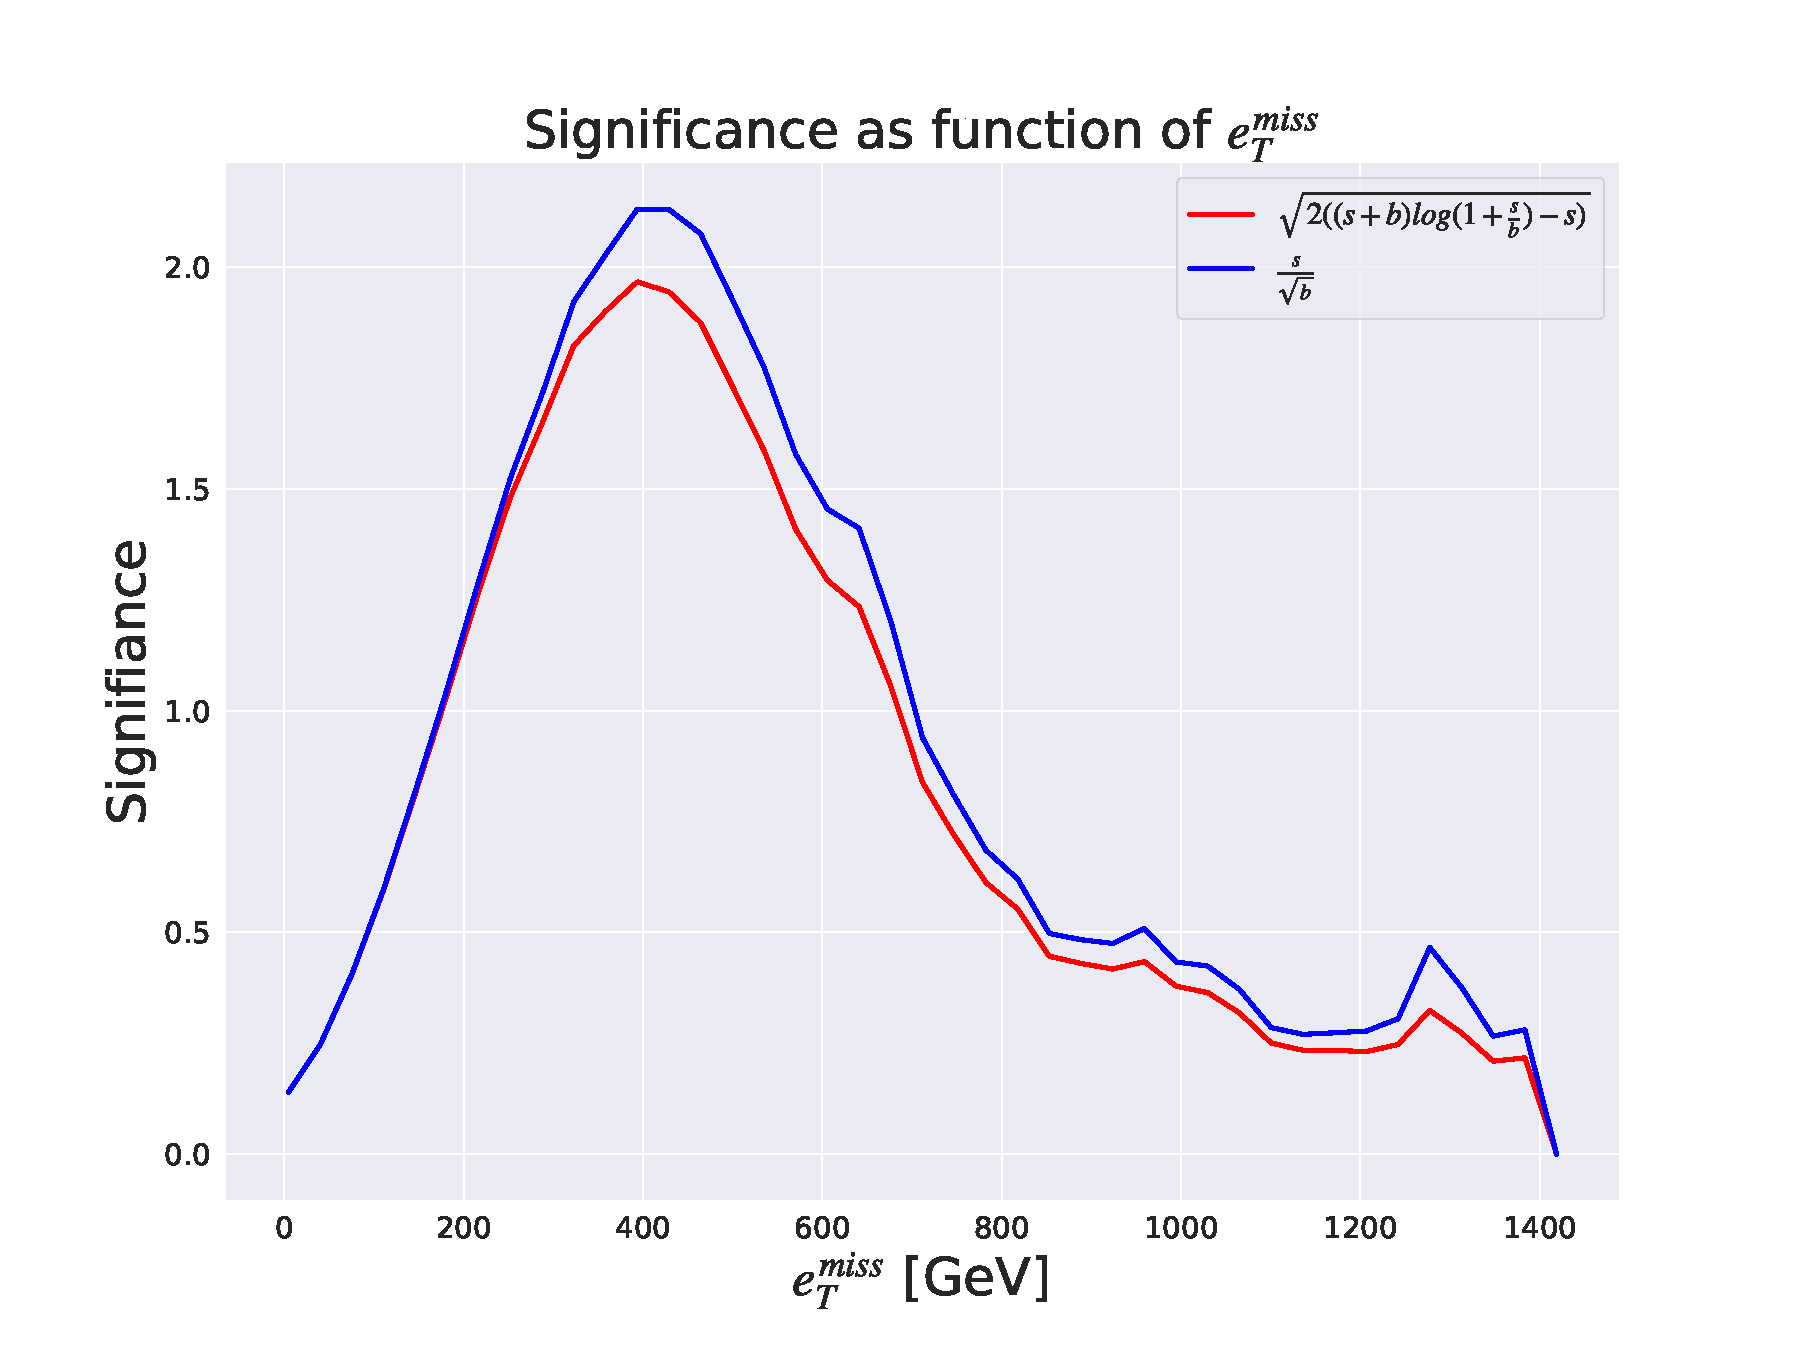
\includegraphics[width=\textwidth]{Figures/VAE_testing/big/3lep/significance_etmiss_450p0p0300_-0.8226861536678497.pdf}
        \caption{}
        \label{fig:VAE_3lep_big_signi_450_2}
    \end{subfigure}
    \hfill      
    \caption[3lep deep network | $450p300$ | VAE | 2]{Reconstruction error, $e_T^{miss}$ signal region, $m_{lll}$ signal region and significance as function of 
    $e_T^{miss}$ for the deep variational autoencoder. Here the SUSY $450p300$ model is used.
    Figure \ref{fig:VAE_3lep_big_450_2} shows the reconstruction error 
    distribution for the SM MC and the SUSY signal. Here the autoencoder produce a bell-shape for background and 
    signal with little destinction. The peaks of the two distributions are not separated in reconstruction error. Figure \ref{fig:VAE_3lep_big_etmiss_450_2} 
    shows the $e_T^{miss}$ distribution for the SM MC and the SUSY signal in the signal region. 
    The signal region is made using a cut around $10^{-0.82}$. Some background is removed, and the peaks of the SM MC and signal 
    distributions are separated. Figure \ref{fig:VAE_3lep_big_mlll_450_2} shows the $m_{lll}$ distribution for the SM MC and the SUSY signal. 
    The shape of both distributions are displaying almost the same shape. Figure \ref{fig:VAE_3lep_big_signi_450_2} shows the significance as 
    function of $e_T^{miss}$. The peak is put around a cut of about 400 GeV in the $e_T^{miss}$, with a significance of around $2.5$.}
    \label{fig:VAE_3lep_big_rec_sig_signi_450_2}
\end{figure}

\begin{figure}[H]
    \centering
    \begin{subfigure}{.40\textwidth}
        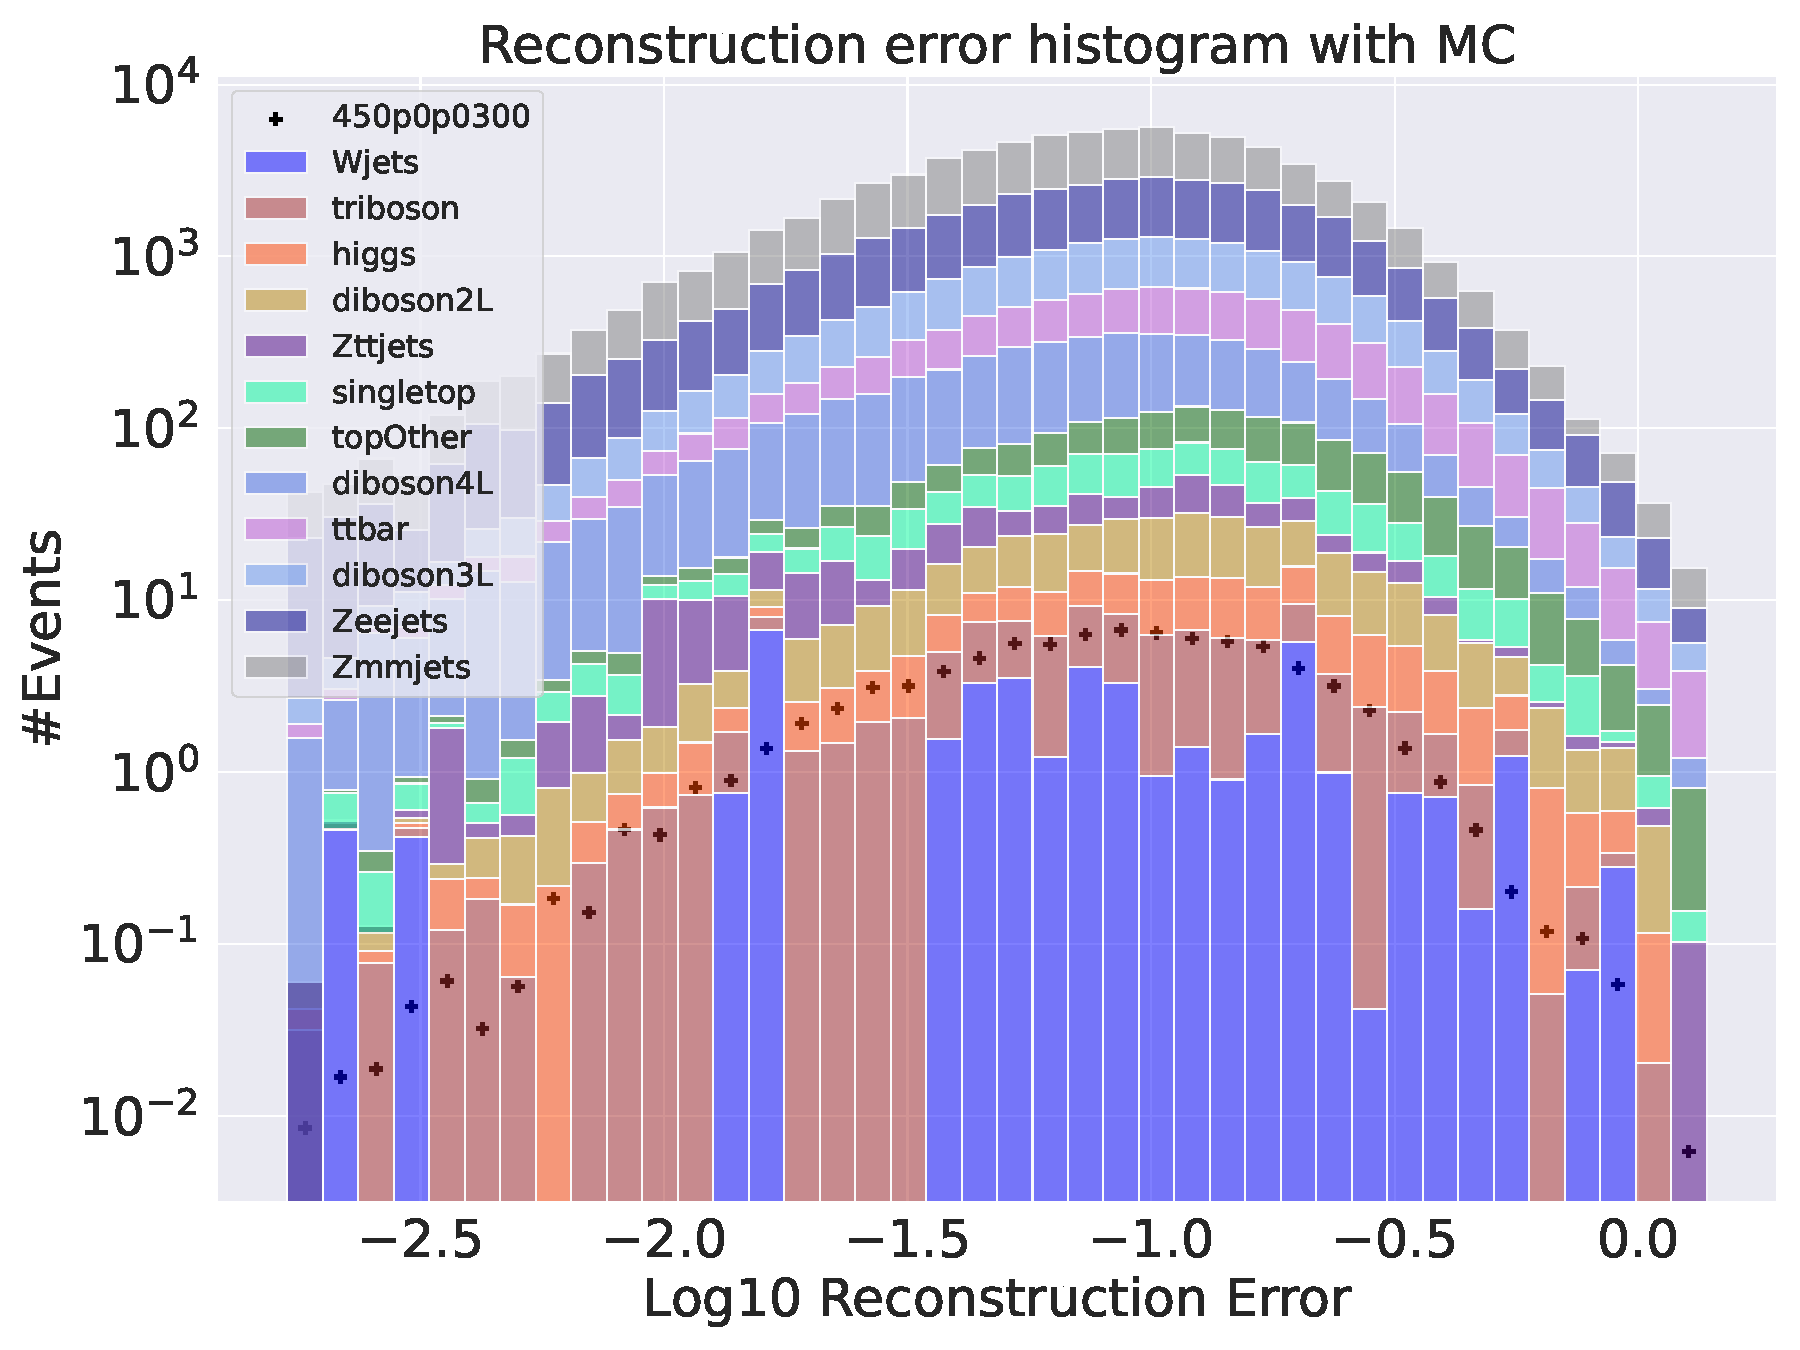
\includegraphics[width=\textwidth]{Figures/VAE_testing/small/3lep/b_data_recon_big_rm3_feats_sig_450p0p0300.pdf}
        \caption{ }
        \label{fig:VAE_3lep_small_450_2}
    \end{subfigure}
    \hfill
    \begin{subfigure}{.40\textwidth}
        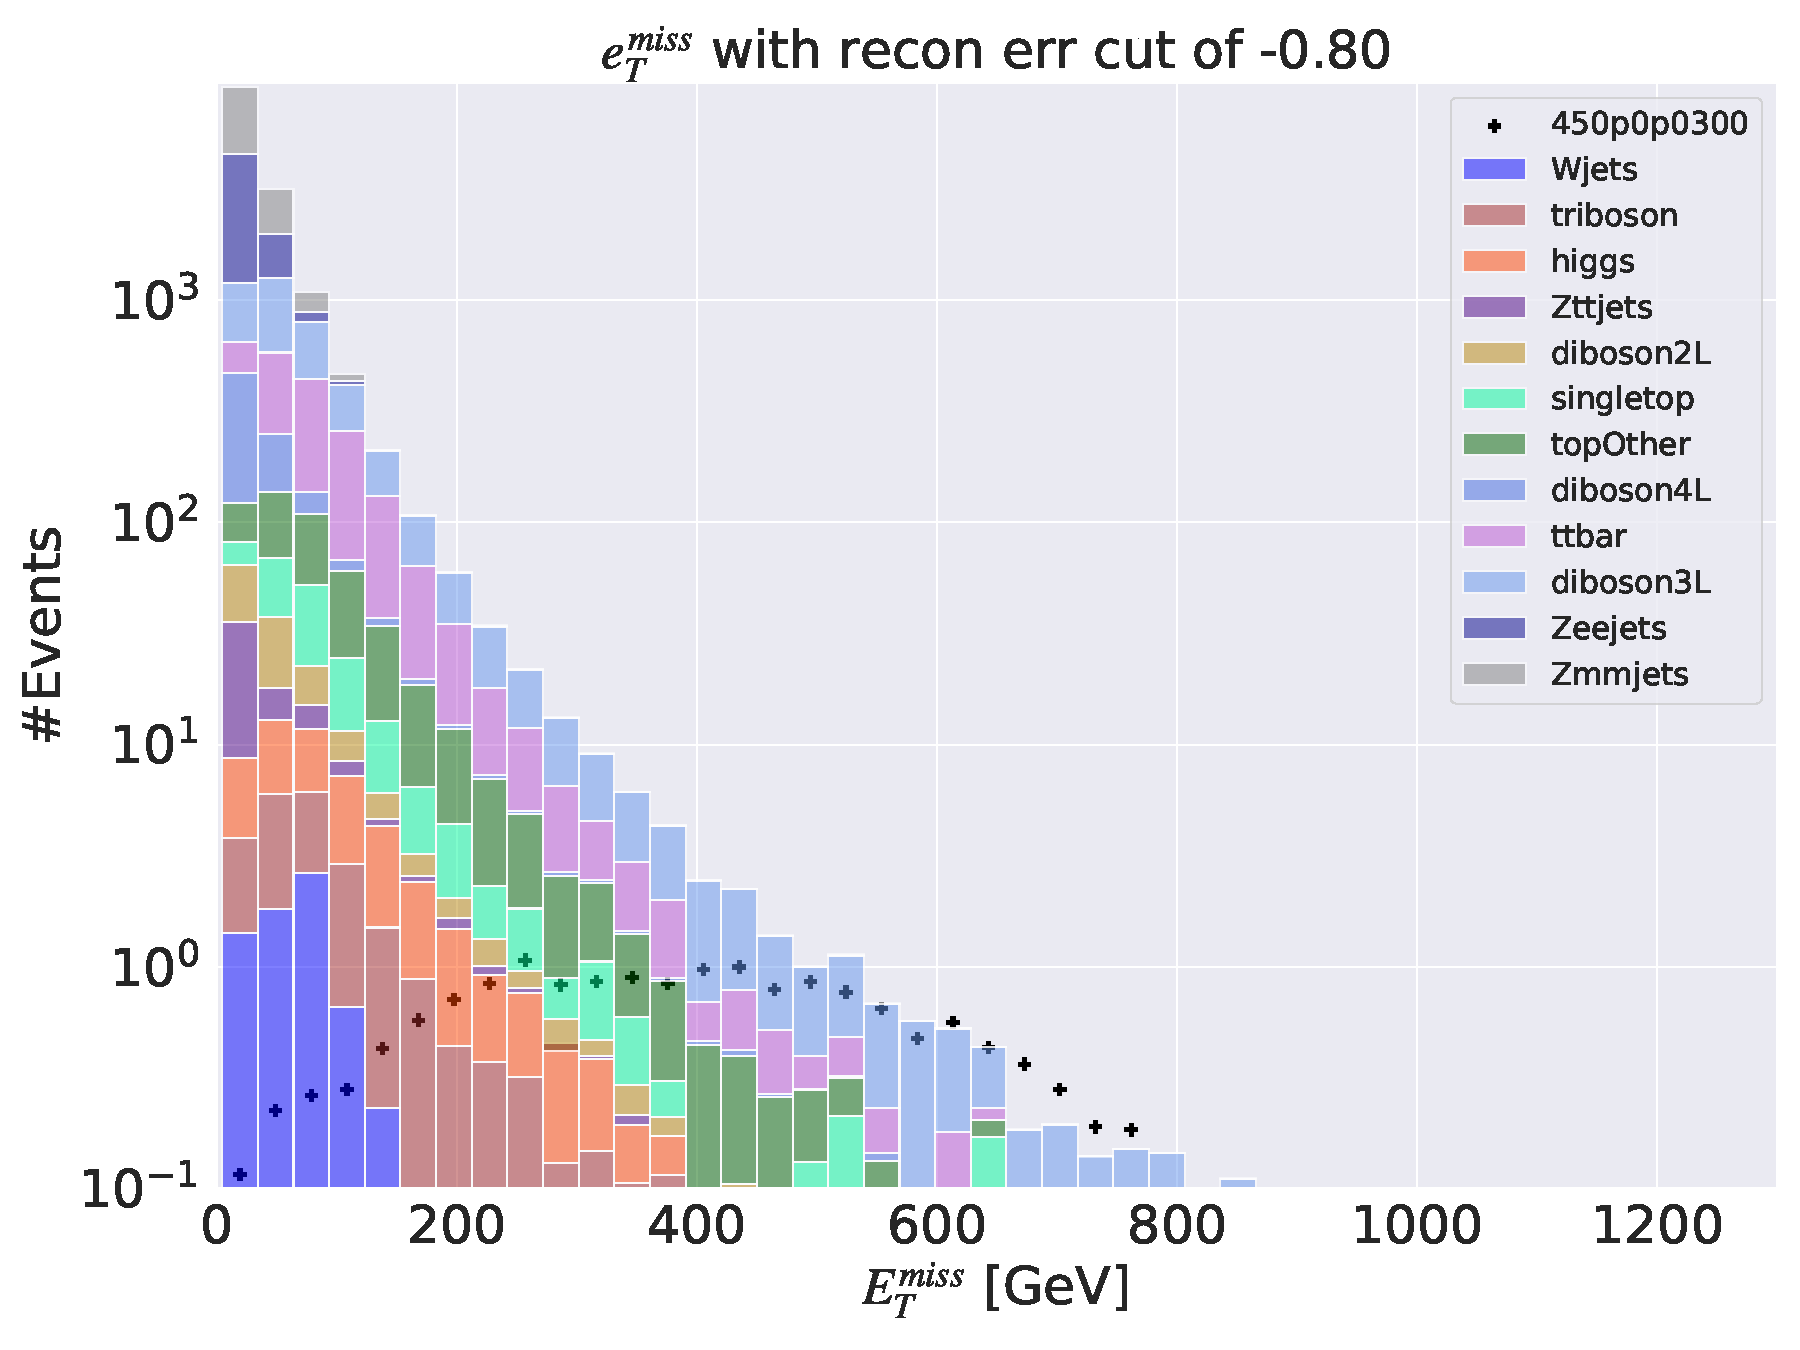
\includegraphics[width=\textwidth]{Figures/VAE_testing/small/3lep/b_data_recon_big_rm3_feats_sig_450p0p0300_etmiss_recon_errcut_-0.80.pdf}
        \caption{}
        \label{fig:VAE_3lep_small_etmiss_450_2}
    \end{subfigure}
    \hfill
    \begin{subfigure}{.40\textwidth}
        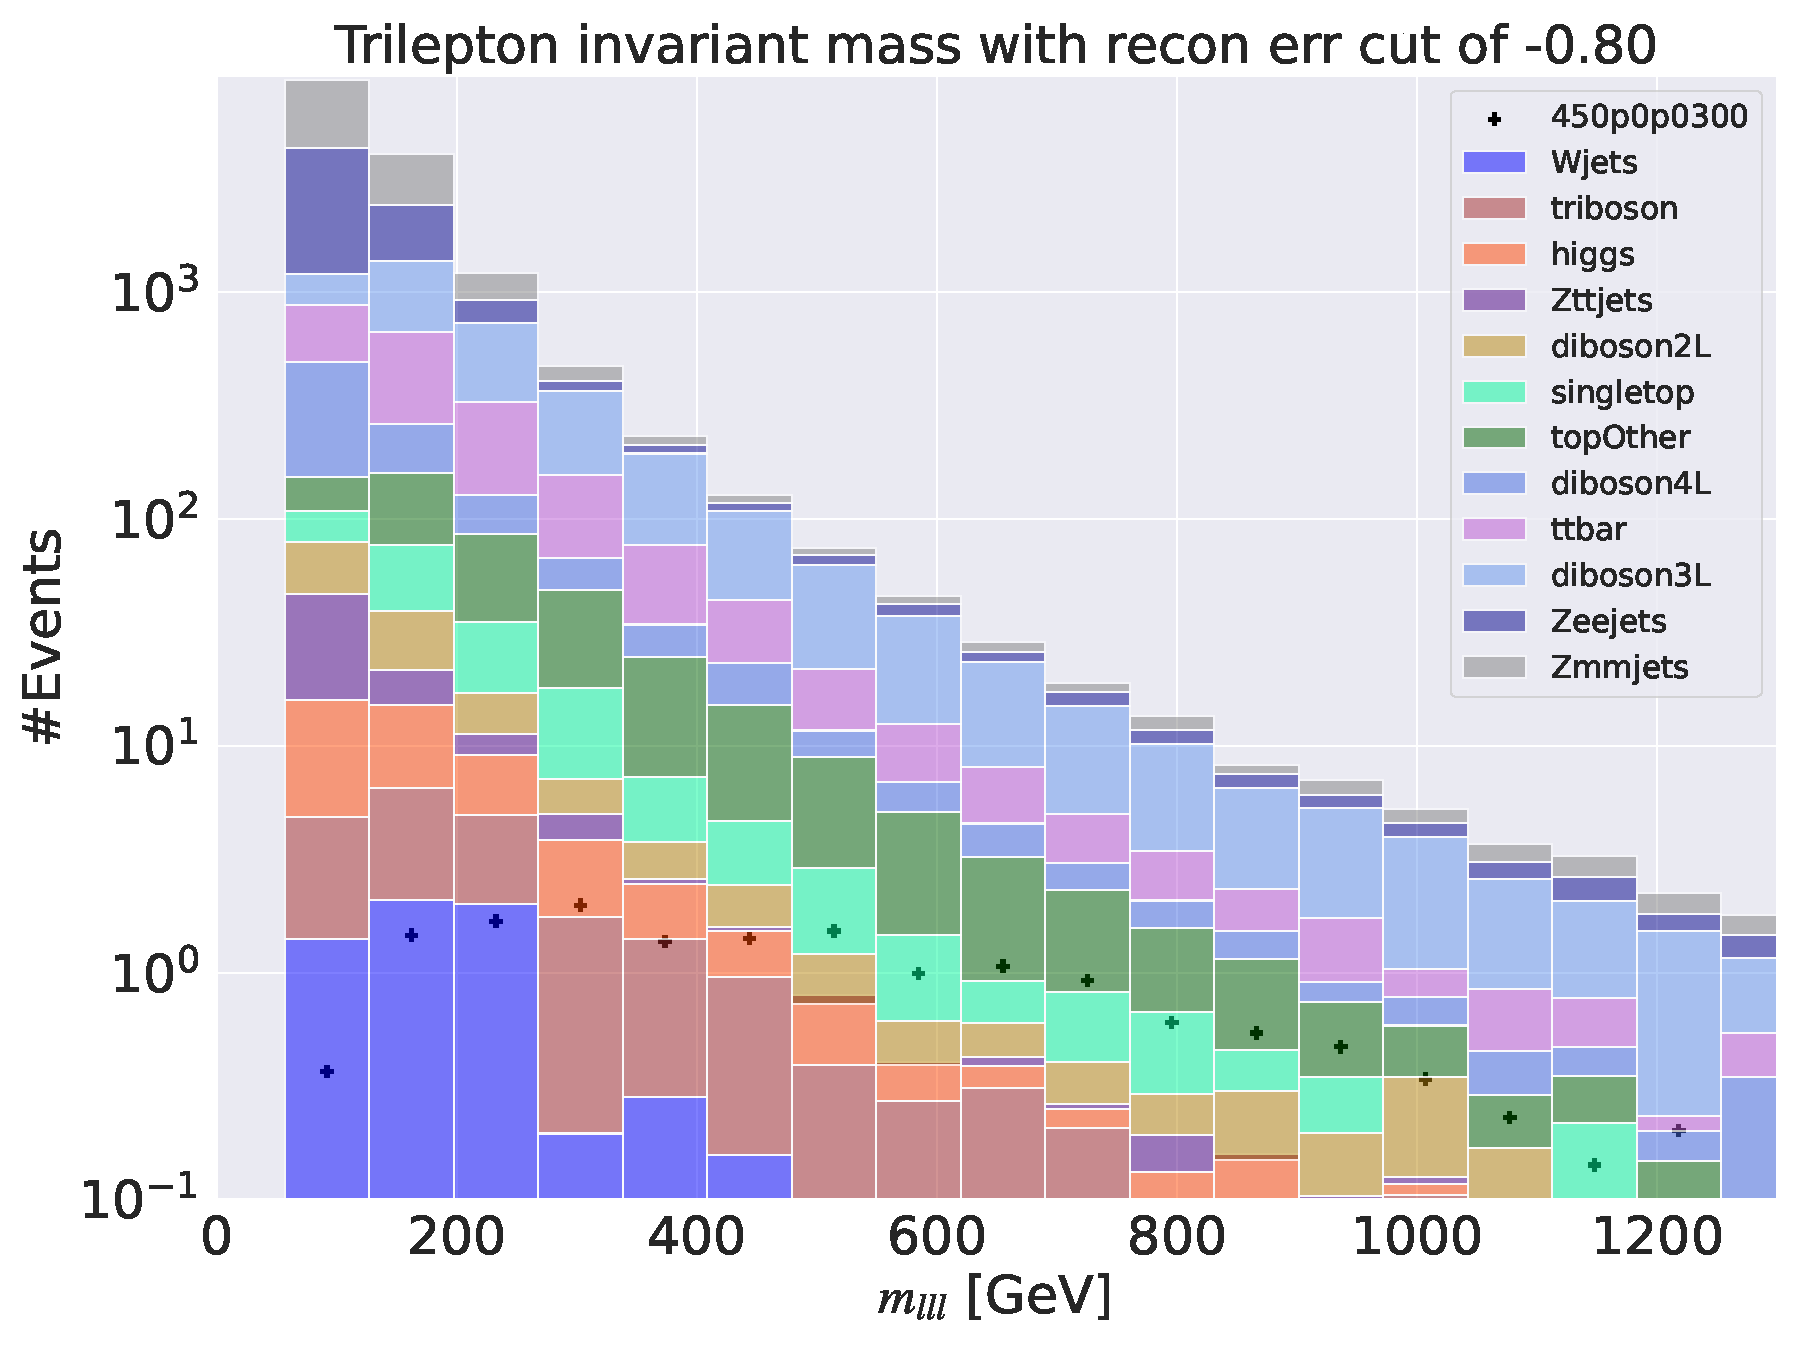
\includegraphics[width=\textwidth]{Figures/VAE_testing/small/3lep/b_data_recon_big_rm3_feats_sig_450p0p0300_mlll_recon_errcut_-0.80.pdf}
        \caption{}
        \label{fig:VAE_3lep_small_mlll_450_2}
    \end{subfigure}
    \hfill   
    \begin{subfigure}{.40\textwidth}
        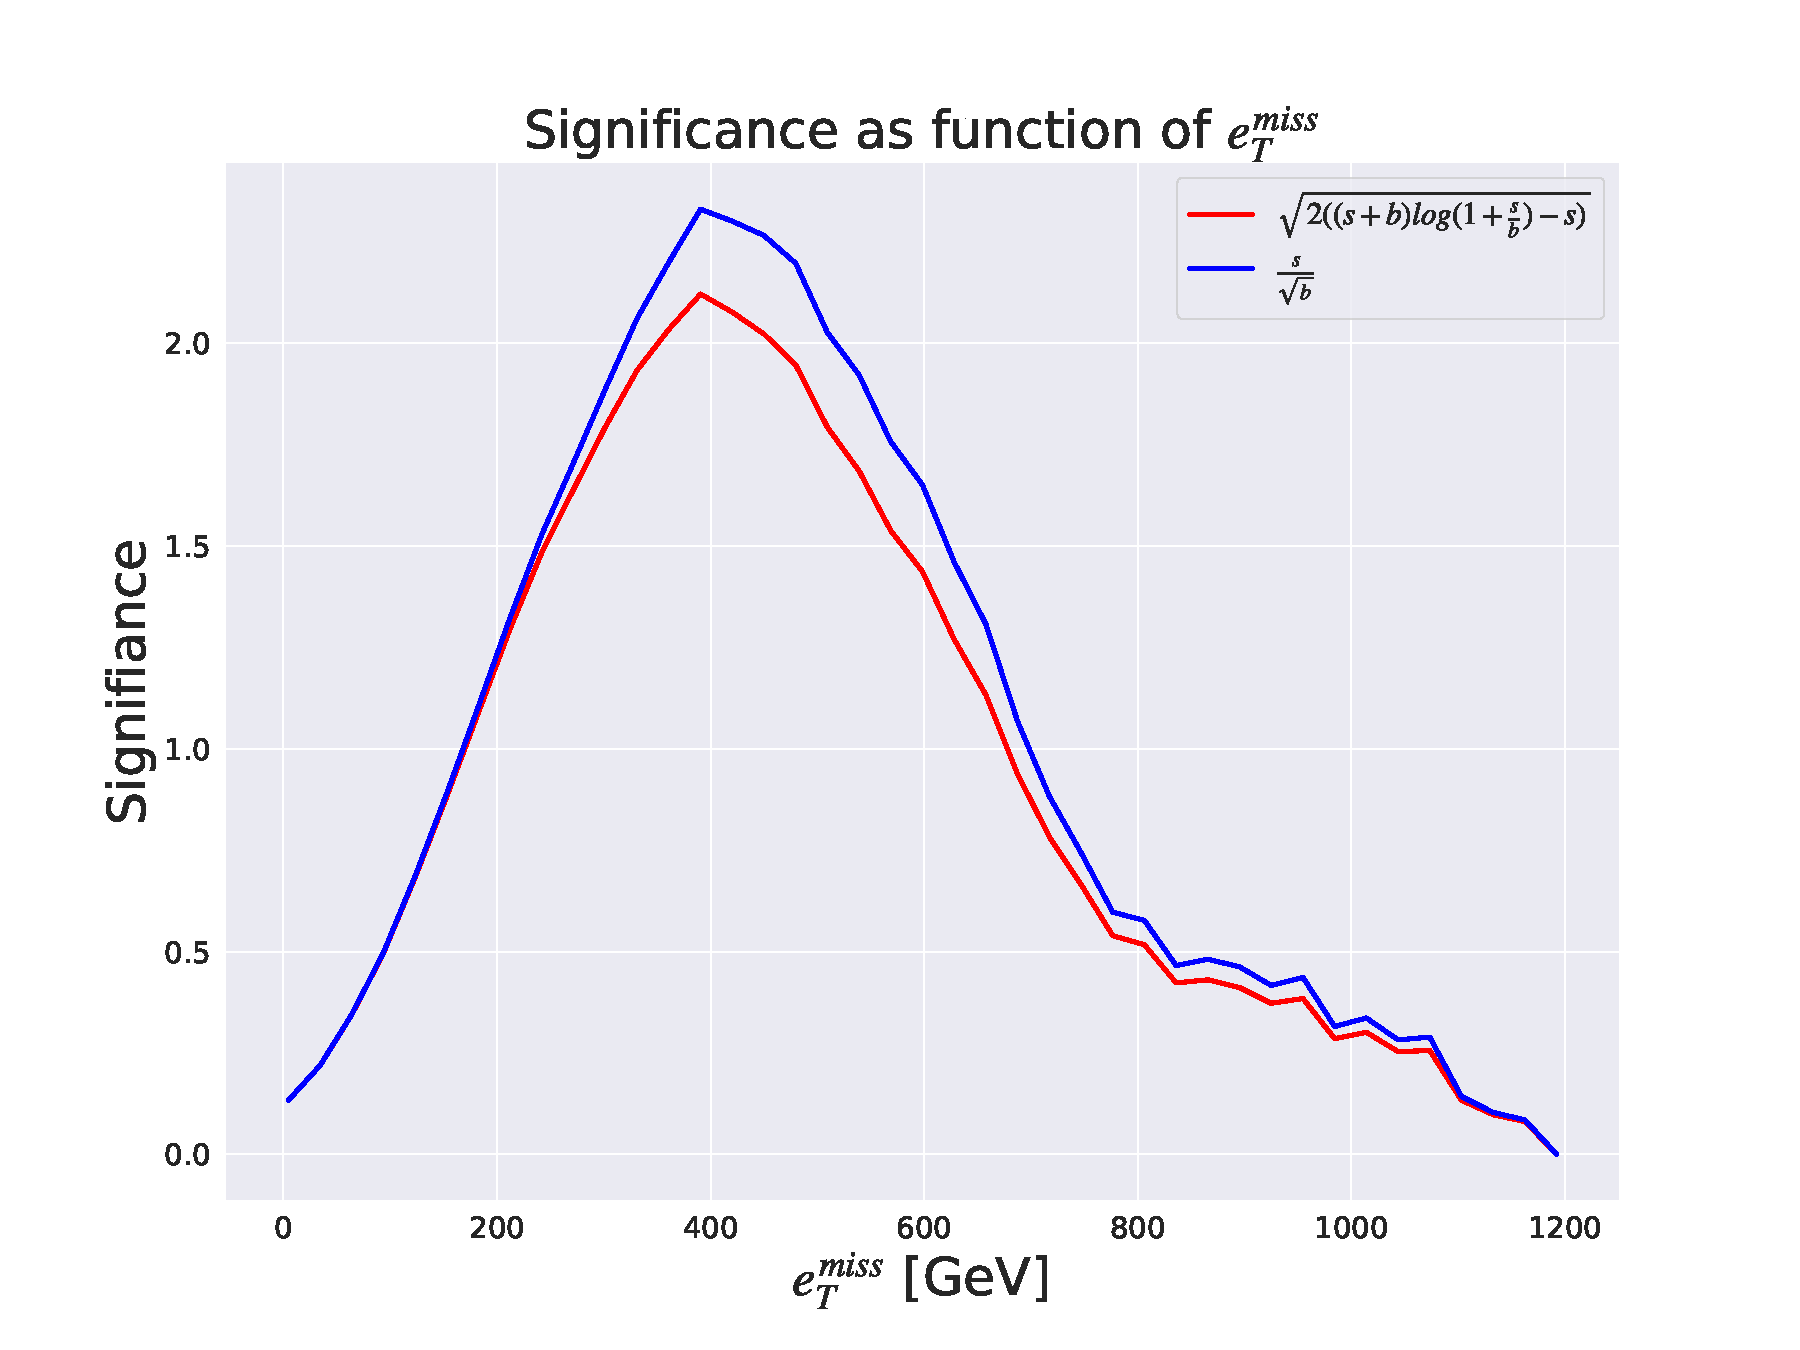
\includegraphics[width=\textwidth]{Figures/VAE_testing/small/3lep/significance_etmiss_450p0p0300_-0.7957779204248656.pdf}
        \caption{}
        \label{fig:VAE_3lep_small_signi_450_2}
    \end{subfigure}
    \hfill      
    \caption[3lep shallow network | $450p300$ | VAE | 2]{Reconstruction error, $e_T^{miss}$ signal region, $m_{lll}$ signal region and significance as function of 
    $e_T^{miss}$ for the shallow variational autoencoder. Here the SUSY $450p300$ model is used.
    Figure \ref{fig:VAE_3lep_small_450_2} shows the reconstruction error 
    distribution for the SM MC and the SUSY signal. Here the autoencoder produce a bell-shape for background and 
    signal with little destinction. The peaks of the two distributions are not separated in reconstruction error. Figure \ref{fig:VAE_3lep_small_etmiss_450_2} 
    shows the $e_T^{miss}$ distribution for the SM MC and the SUSY signal in the signal region. 
    The signal region is made using a cut around $10^{-0.80}$. Some background is removed, and the peaks of the SM MC and signal 
    distributions are separated. Figure \ref{fig:VAE_3lep_small_mlll_450_2} shows the $m_{lll}$ distribution for the SM MC and the SUSY signal. 
    The shape of both distributions are displaying almost the same shape. Figure \ref{fig:VAE_3lep_small_signi_450_2} shows the significance as 
    function of $e_T^{miss}$. The peak is put around a cut of about 400 GeV in the $e_T^{miss}$, with a significance of around $2.6$.}
    \label{fig:VAE_3lep_small_rec_sig_signi_450_2}
\end{figure}








\begin{figure}[H]
    \centering
    \begin{subfigure}{.40\textwidth}
        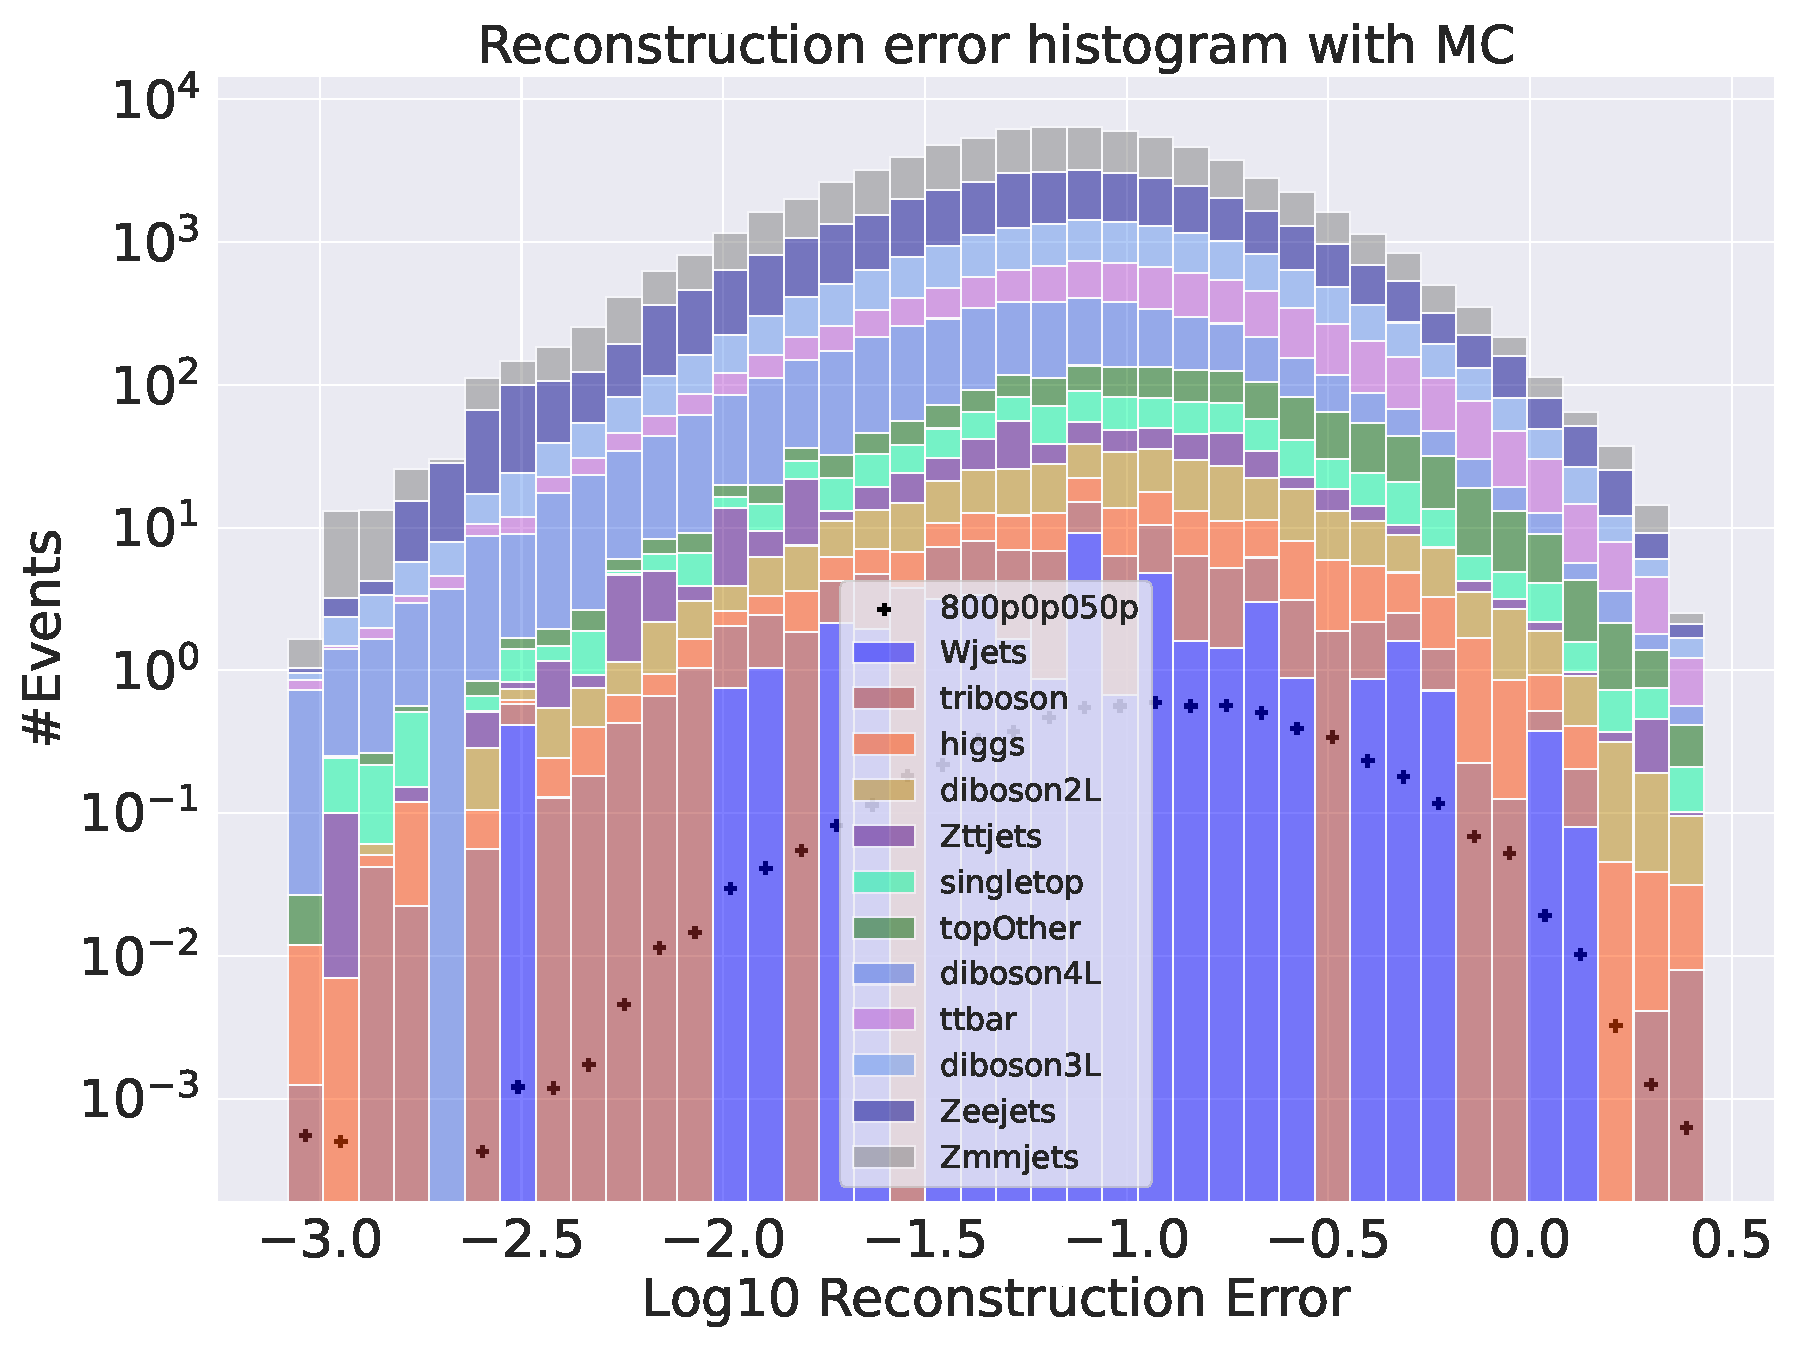
\includegraphics[width=\textwidth]{Figures/VAE_testing/big/3lep/b_data_recon_big_rm3_feats_sig_800p0p050p.pdf}
        \caption{ }
        \label{fig:VAE_3lep_big_800_2}
    \end{subfigure}
    \hfill
    \begin{subfigure}{.40\textwidth}
        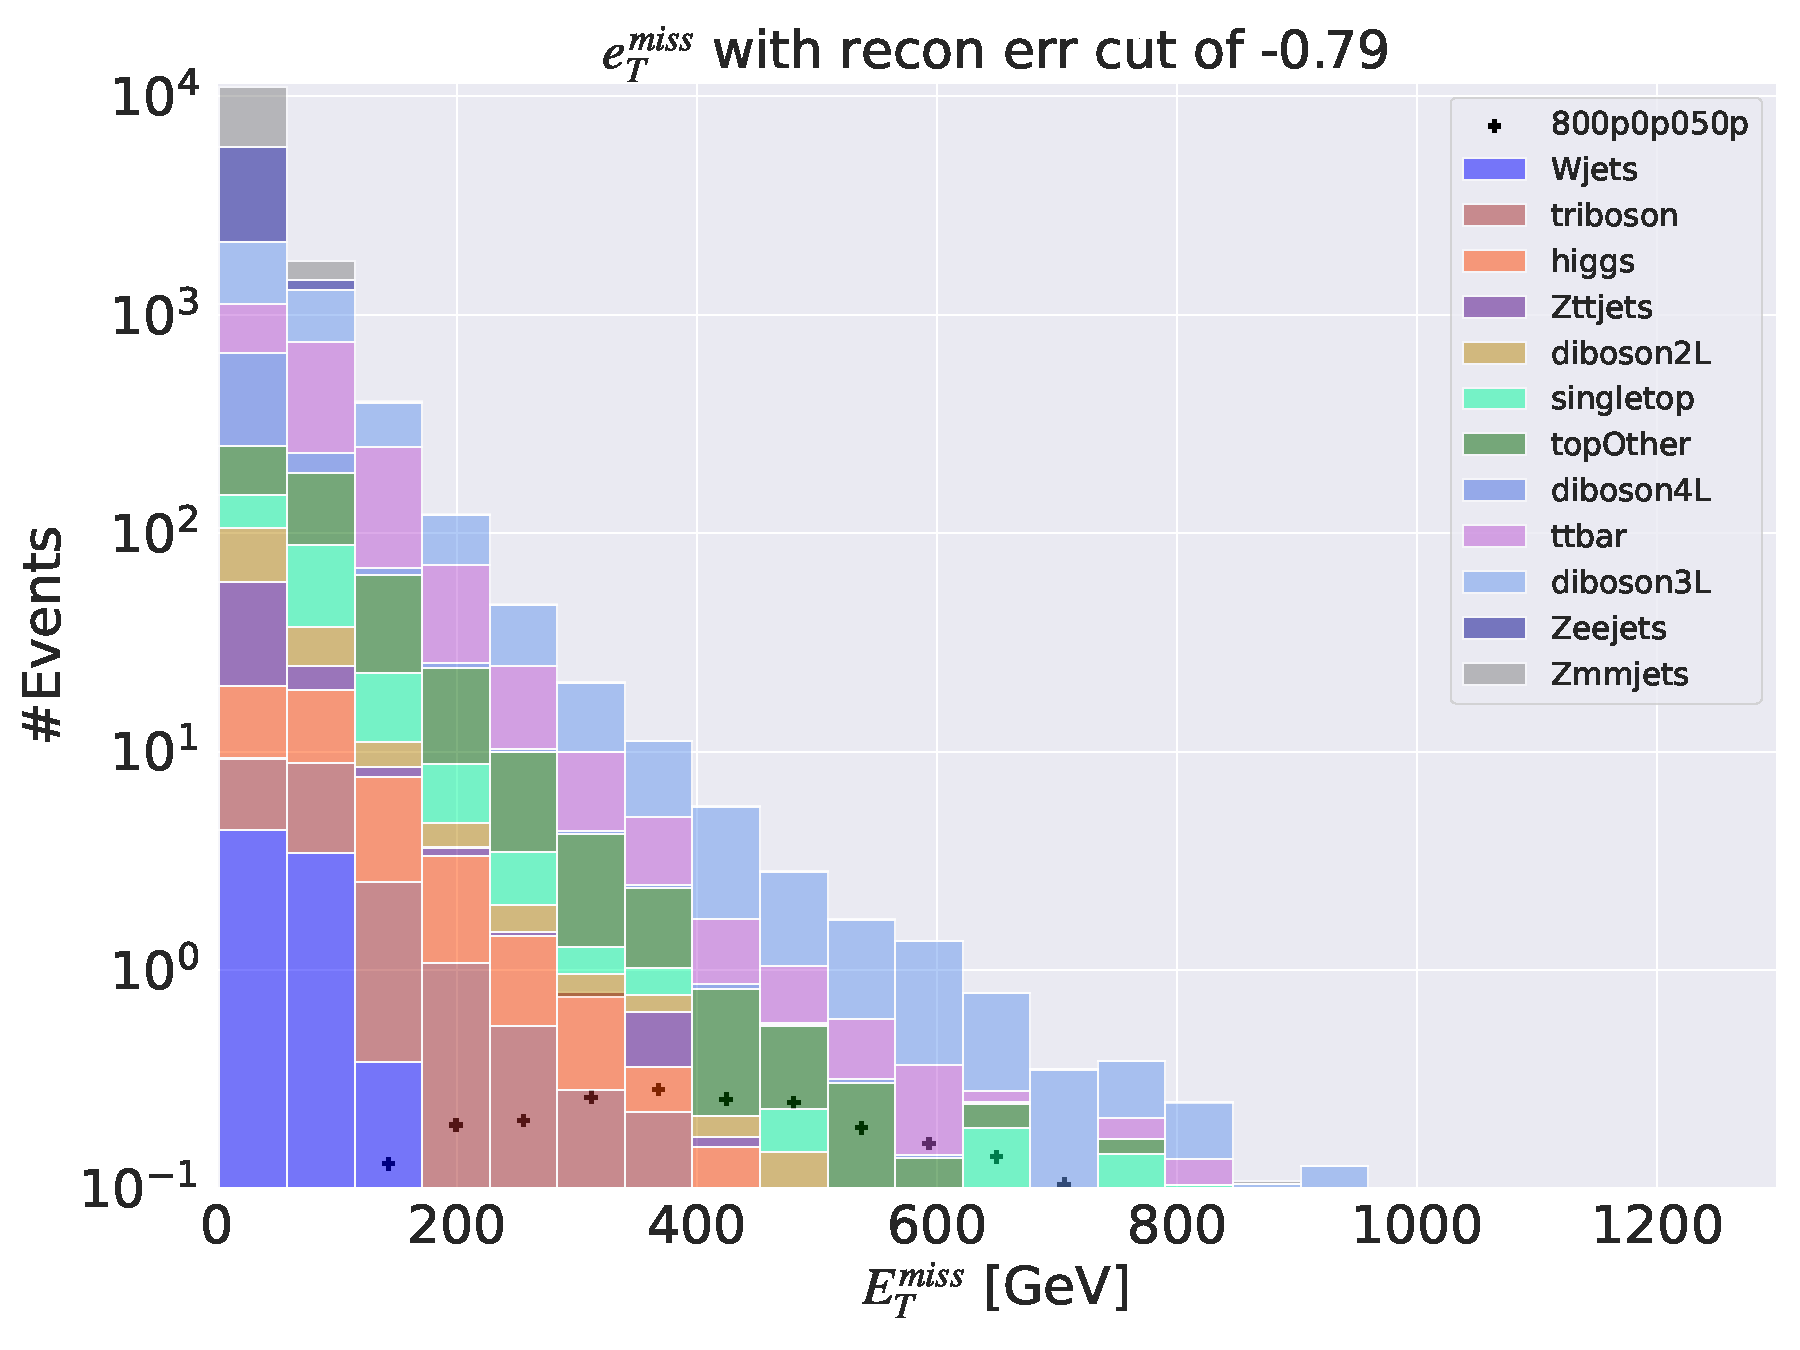
\includegraphics[width=\textwidth]{Figures/VAE_testing/big/3lep/b_data_recon_big_rm3_feats_sig_800p0p050p_etmiss_recon_errcut_-0.79.pdf}
        \caption{}
        \label{fig:VAE_3lep_big_etmiss_800_2}
    \end{subfigure}
    \hfill
    \begin{subfigure}{.40\textwidth}
        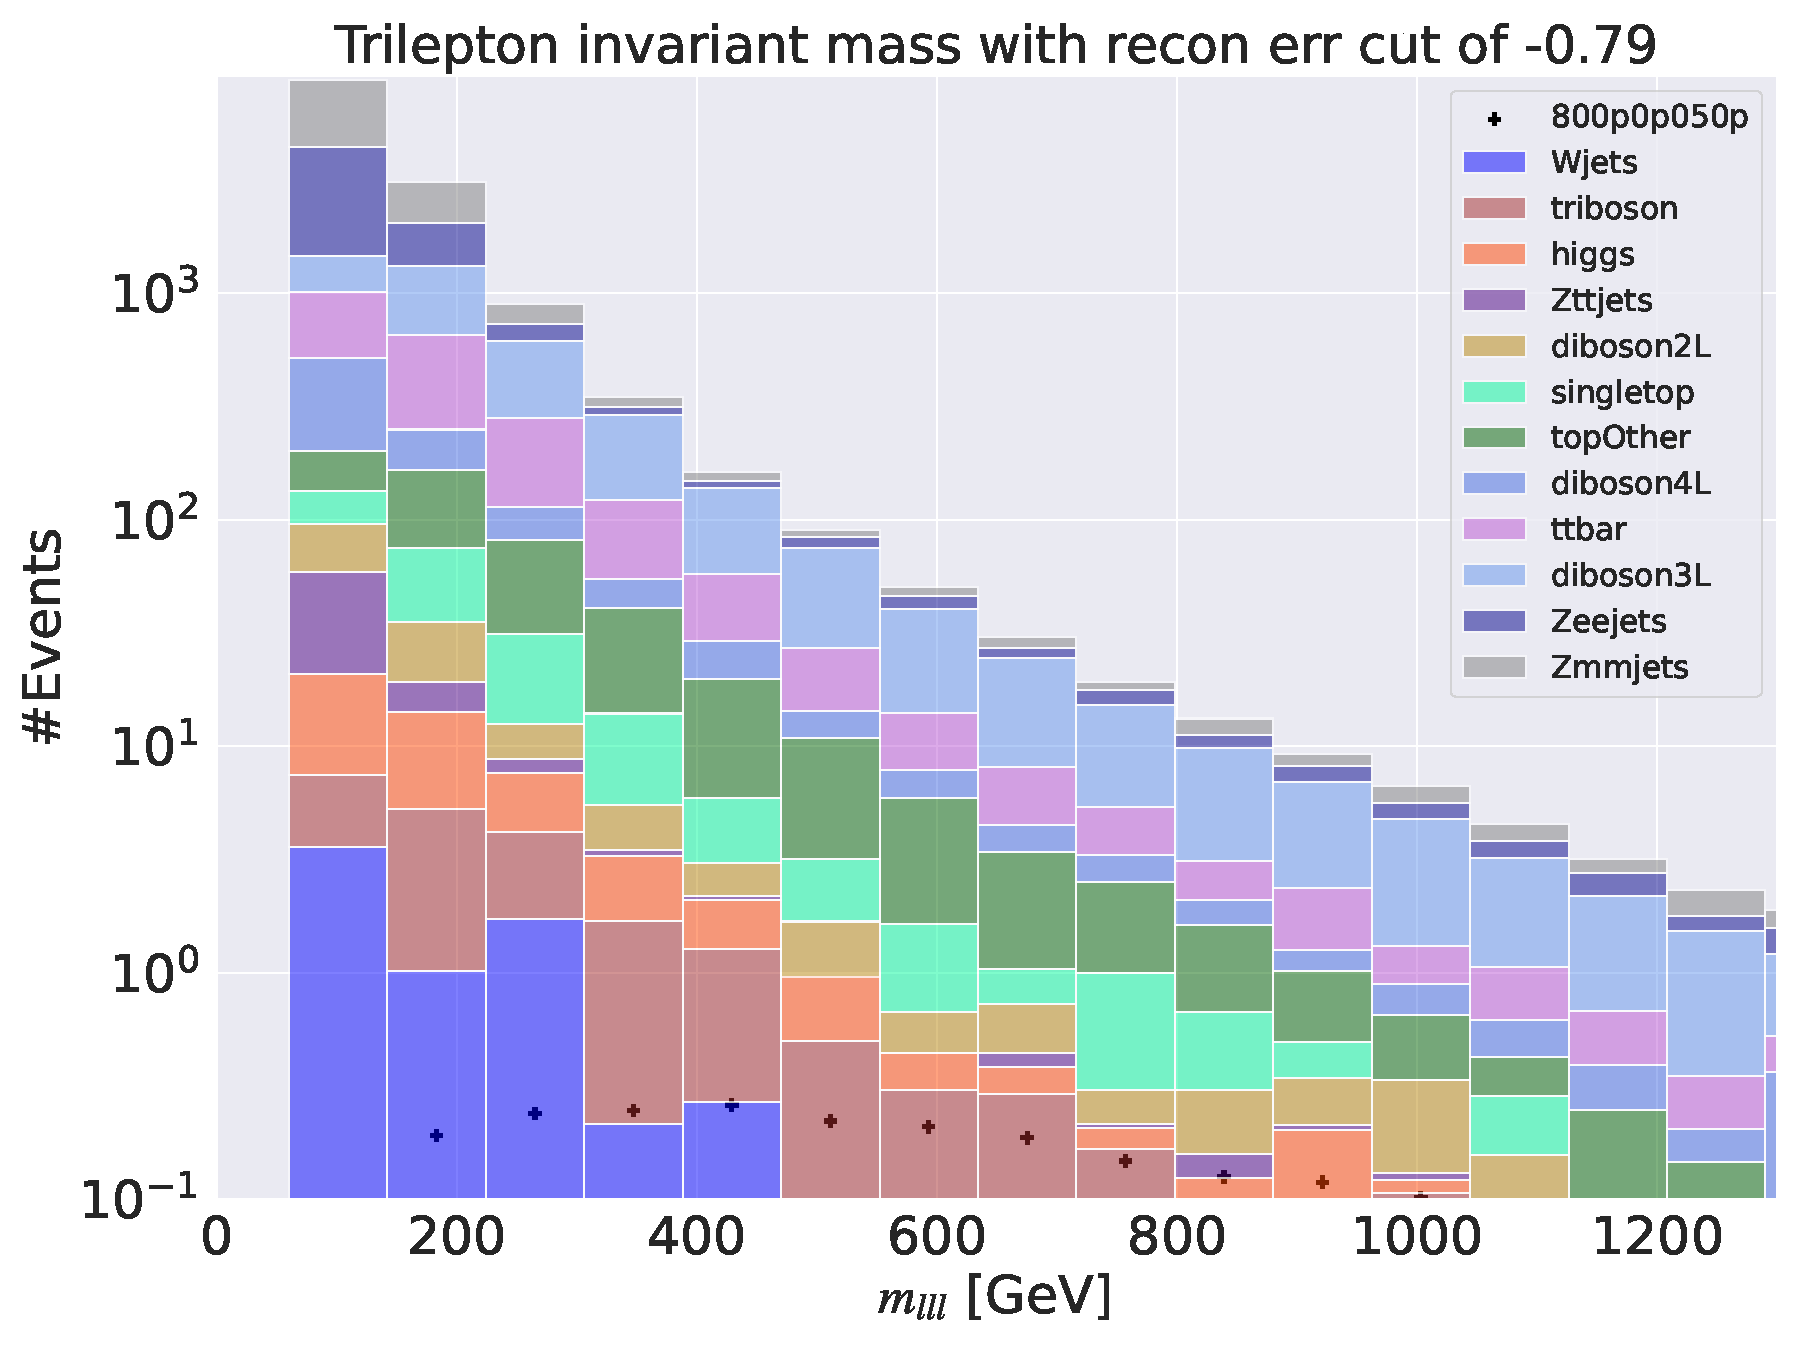
\includegraphics[width=\textwidth]{Figures/VAE_testing/big/3lep/b_data_recon_big_rm3_feats_sig_800p0p050p_mlll_recon_errcut_-0.79.pdf}
        \caption{}
        \label{fig:VAE_3lep_big_mlll_800_2}
    \end{subfigure}
    \hfill   
    \begin{subfigure}{.40\textwidth}
        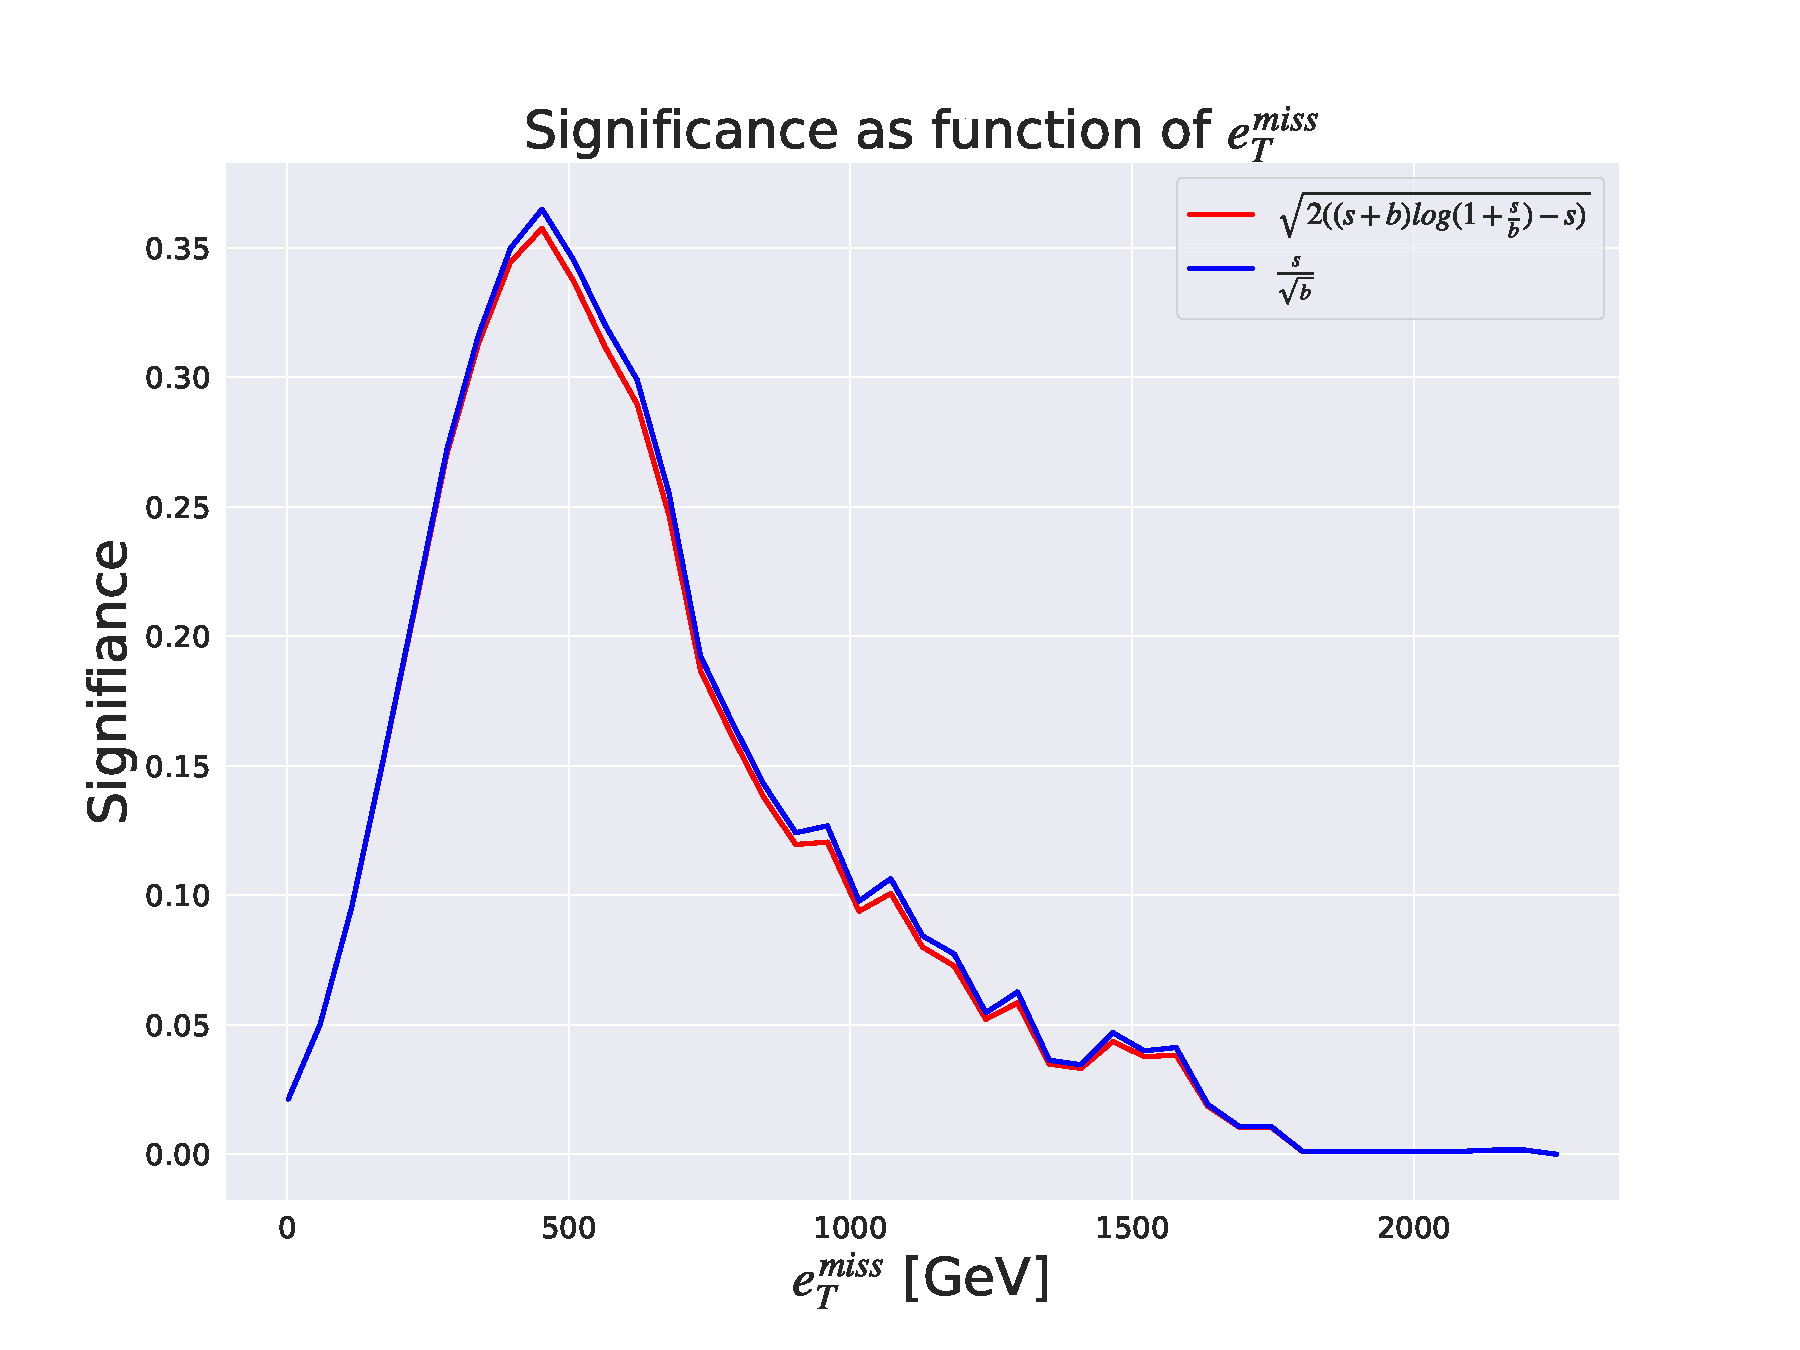
\includegraphics[width=\textwidth]{Figures/VAE_testing/big/3lep/significance_etmiss_800p0p050p_-0.7941392653620614.pdf}
        \caption{}
        \label{fig:VAE_3lep_big_signi_800_2}
    \end{subfigure}
    \hfill      
    \caption[3lep deep network | $800p50$ | VAE | 2]{Reconstruction error, $e_T^{miss}$ signal region, $m_{lll}$ signal region and significance as function of 
    $e_T^{miss}$ for the deep variational autoencoder. Here the SUSY $450p300$ model is used. 
    Figure \ref{fig:VAE_3lep_big_800_2} shows the reconstruction error 
    distribution for the SM MC and the SUSY signal. Here the autoencoder produce a bell-shape for background and 
    signal with little destinction. The peaks of the two distributions are not separated in reconstruction error. Figure \ref{fig:VAE_3lep_big_etmiss_800_2} 
    shows the $e_T^{miss}$ distribution for the SM MC and the SUSY signal in the signal region. 
    The signal region is made using a cut around $10^{-0.79}$. Some background is removed, and the peaks of the SM MC and signal 
    distributions are separated. Figure \ref{fig:VAE_3lep_big_mlll_800_2} shows the $m_{lll}$ distribution for the SM MC and the SUSY signal. 
    The shape of both distributions are displaying almost the same shape. Figure \ref{fig:VAE_3lep_big_signi_800_2} shows the significance as 
    function of $e_T^{miss}$. The peak is put around a cut of about 400 GeV in the $e_T^{miss}$, with a significance of around $3.3$.}
    \label{fig:VAE_3lep_big_rec_sig_signi_800_2}
\end{figure}

\begin{figure}[H]
    \centering
    \begin{subfigure}{.40\textwidth}
        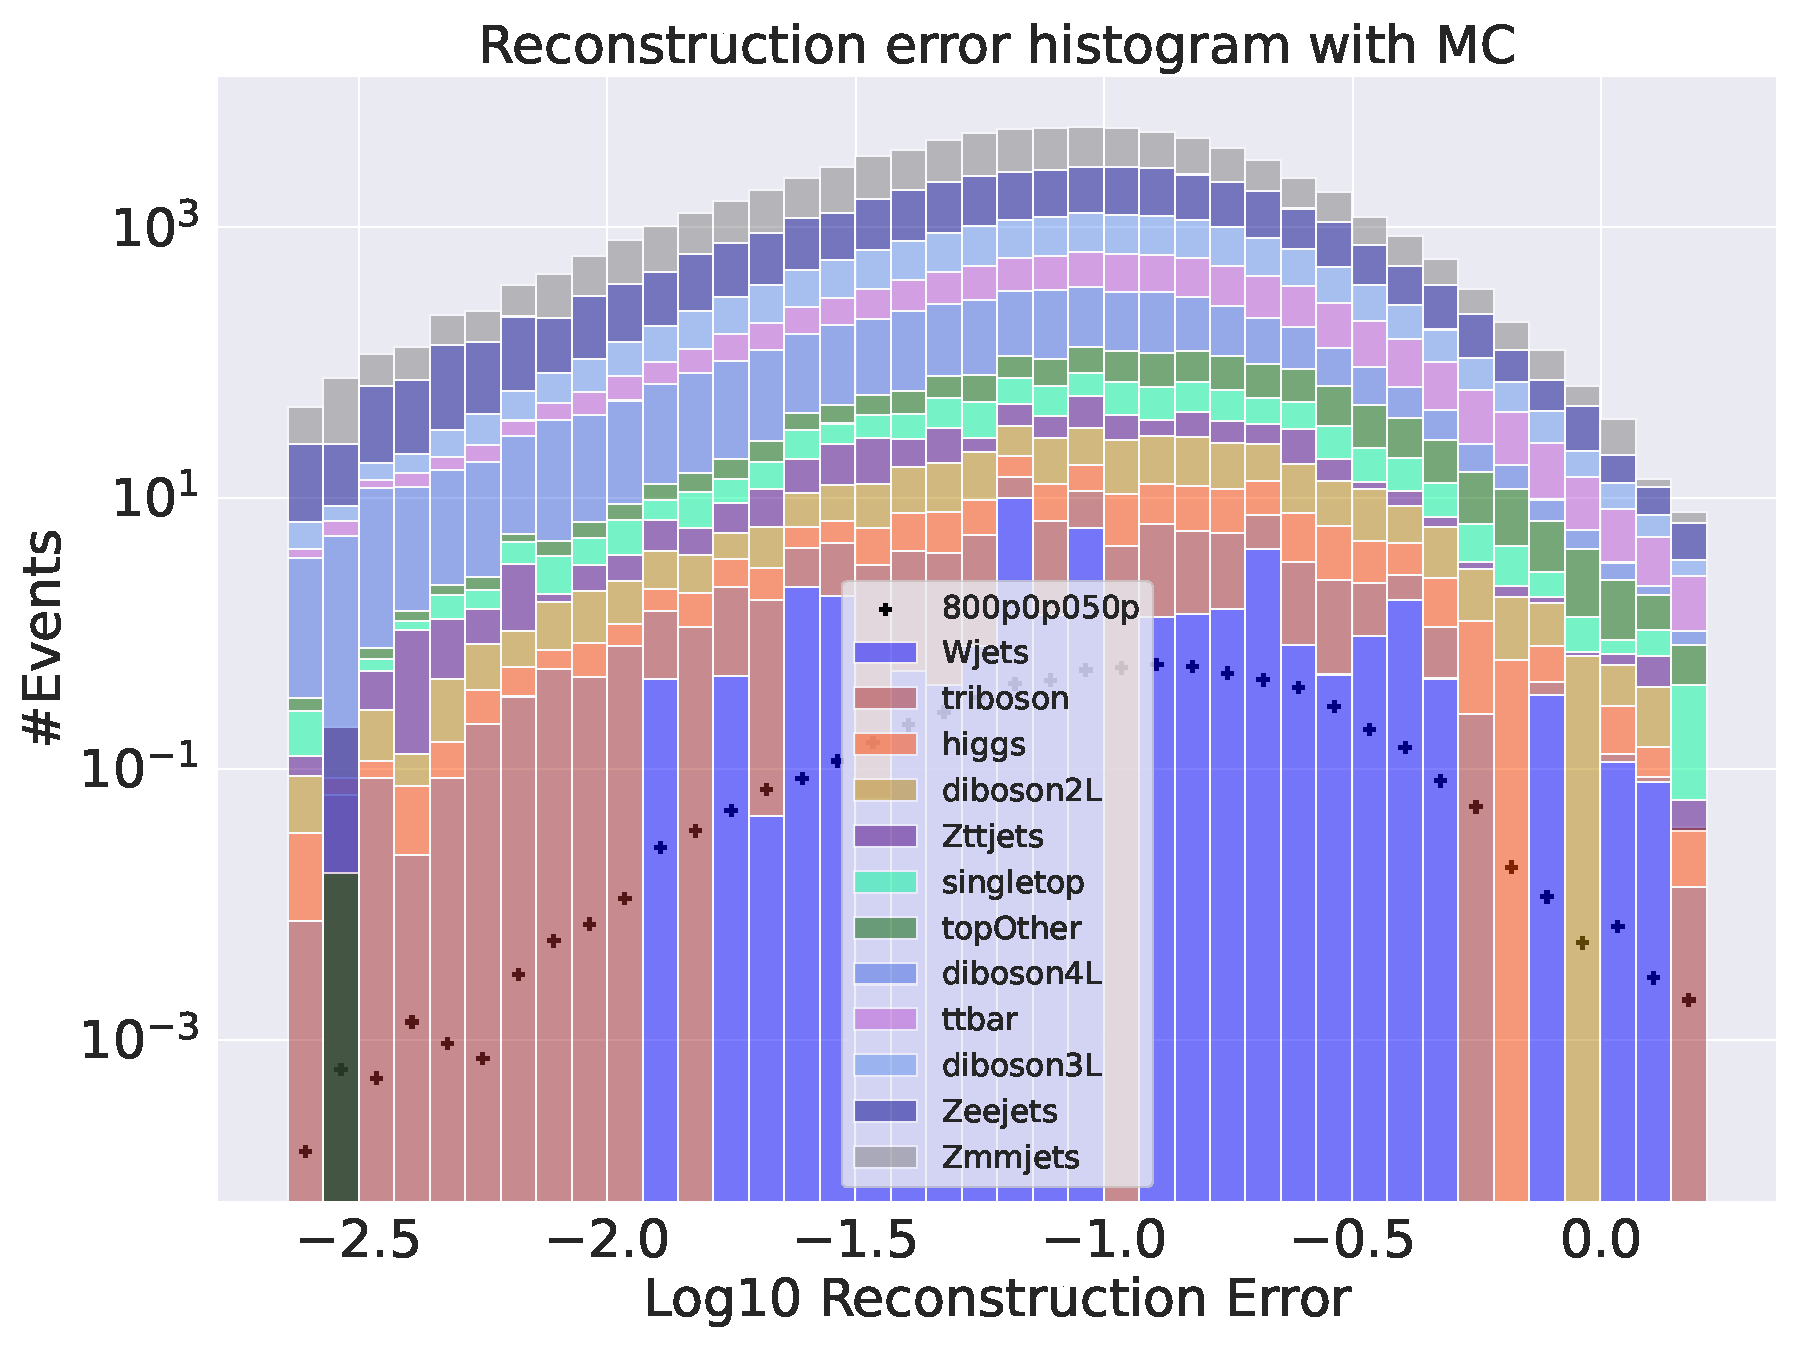
\includegraphics[width=\textwidth]{Figures/VAE_testing/small/3lep/b_data_recon_big_rm3_feats_sig_800p0p050p.pdf}
        \caption{ }
        \label{fig:VAE_3lep_small_800_2}
    \end{subfigure}
    \hfill
    \begin{subfigure}{.40\textwidth}
        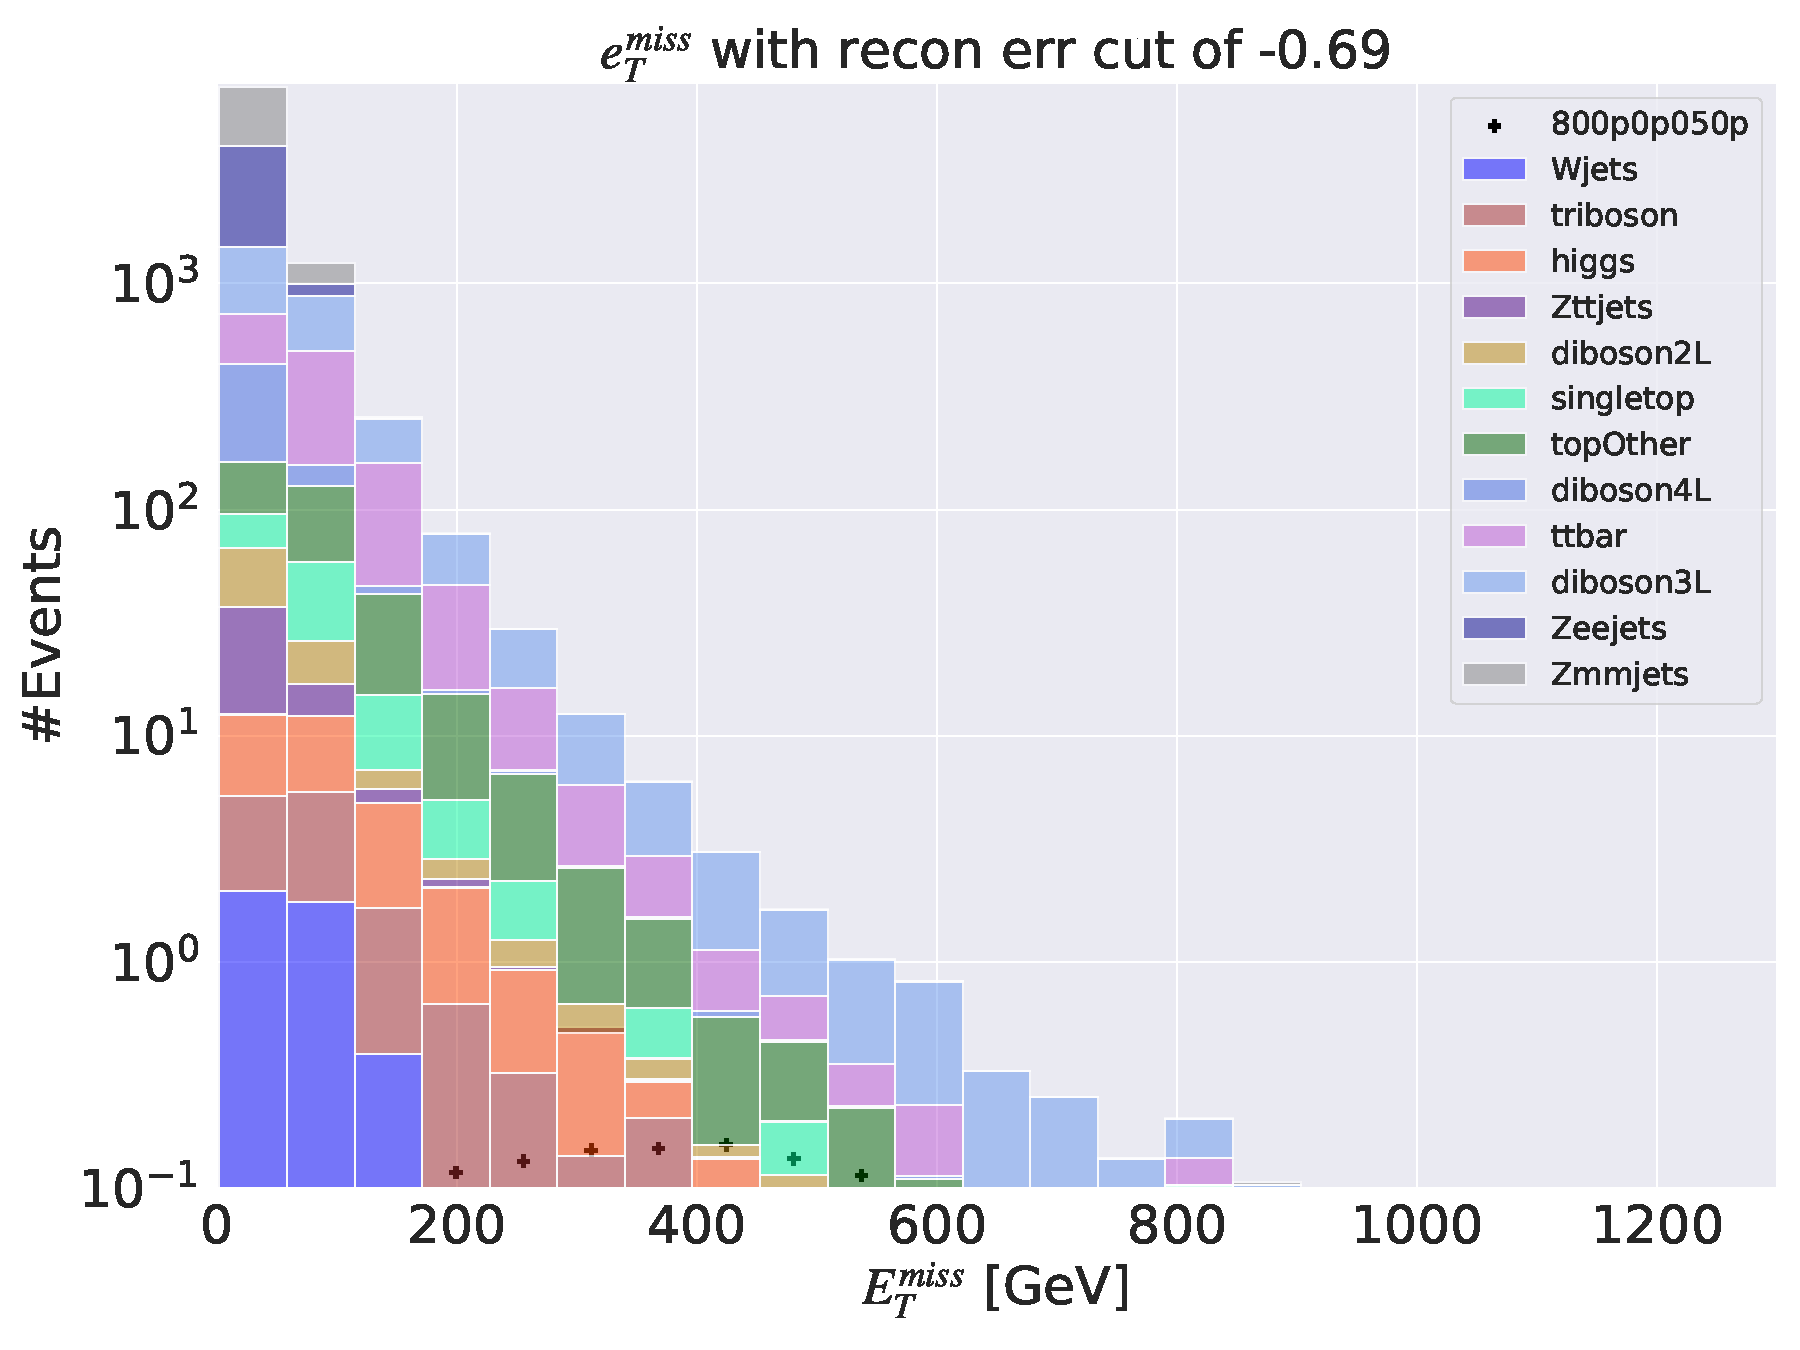
\includegraphics[width=\textwidth]{Figures/VAE_testing/small/3lep/b_data_recon_big_rm3_feats_sig_800p0p050p_etmiss_recon_errcut_-0.69.pdf}
        \caption{}
        \label{fig:VAE_3lep_small_etmiss_800_2}
    \end{subfigure}
    \hfill
    \begin{subfigure}{.40\textwidth}
        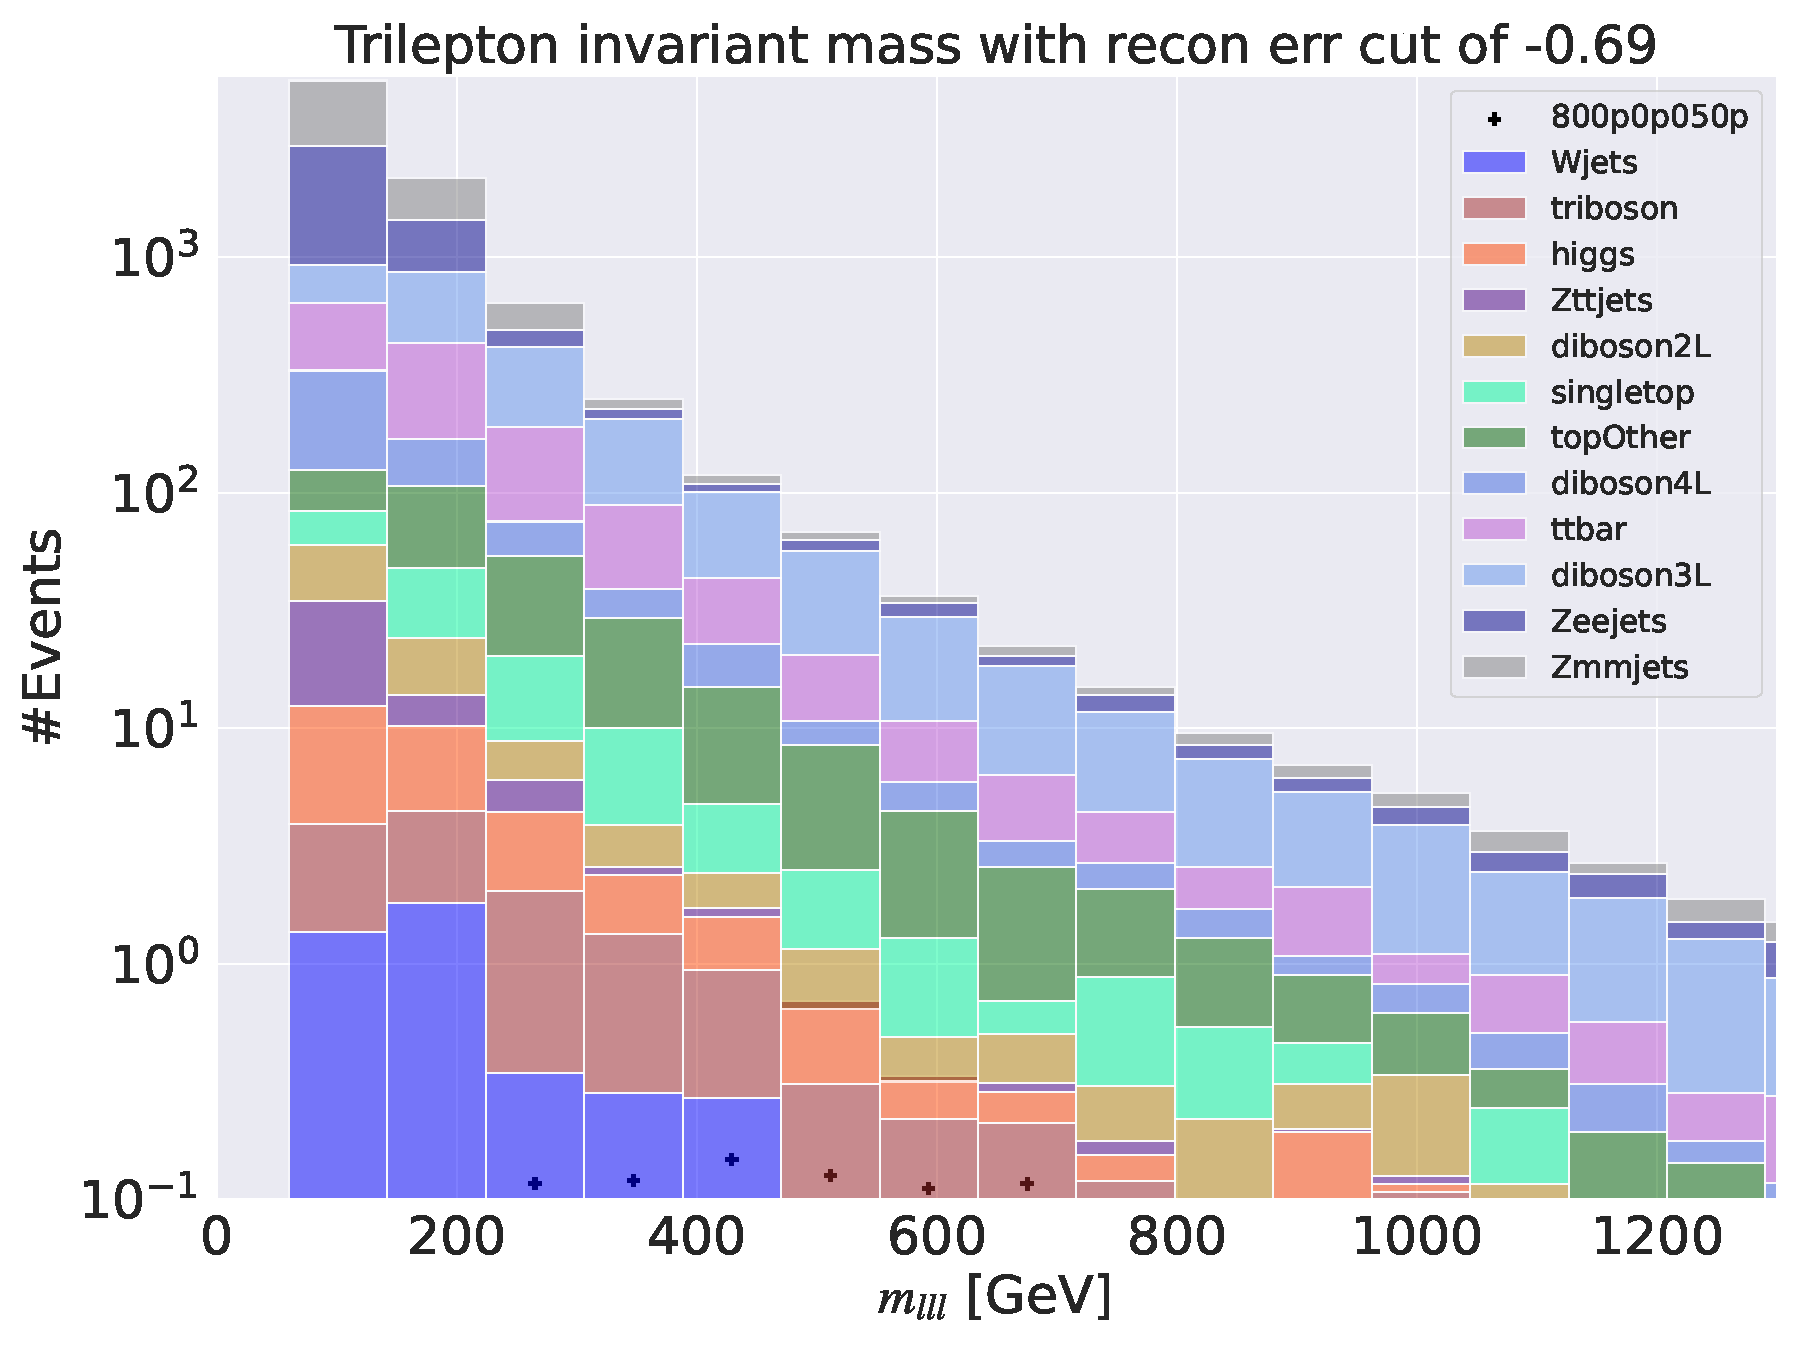
\includegraphics[width=\textwidth]{Figures/VAE_testing/small/3lep/b_data_recon_big_rm3_feats_sig_800p0p050p_mlll_recon_errcut_-0.69.pdf}
        \caption{}
        \label{fig:VAE_3lep_small_mlll_800_2}
    \end{subfigure}
    \hfill   
    \begin{subfigure}{.40\textwidth}
        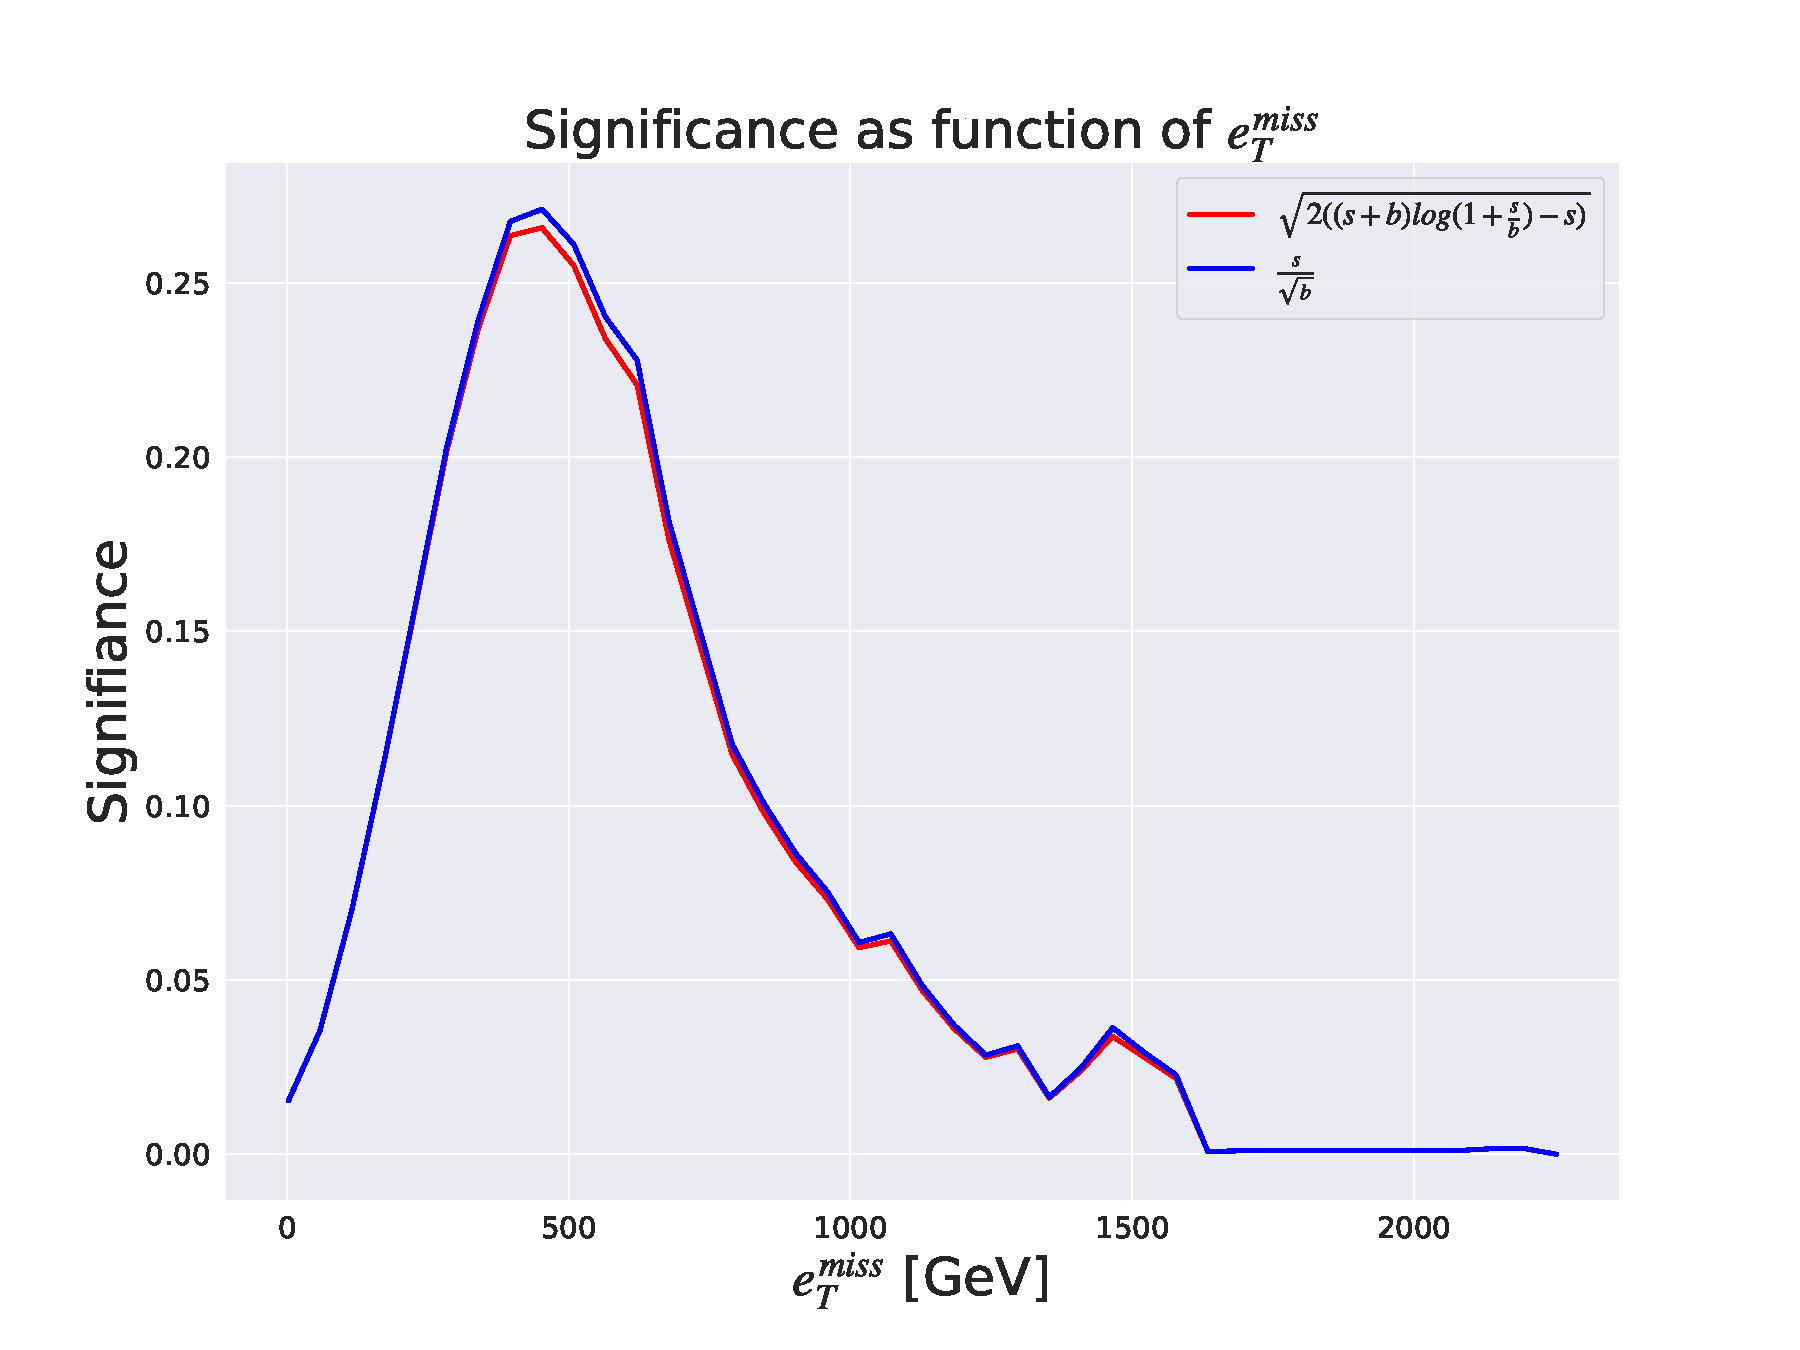
\includegraphics[width=\textwidth]{Figures/VAE_testing/small/3lep/significance_etmiss_800p0p050p_-0.6856921439167579.pdf}
        \caption{}
        \label{fig:VAE_3lep_small_signi_800_2}
    \end{subfigure}
    \hfill      
    \caption[3lep shallow network | $800p50$ | VAE | 2]{Reconstruction error, $e_T^{miss}$ signal region, $m_{lll}$ signal region and significance as function of 
    $e_T^{miss}$ for the shallow variational autoencoder. Here the SUSY $450p300$ model is used.
    Figure \ref{fig:VAE_3lep_small_800_2} shows the reconstruction error 
    distribution for the SM MC and the SUSY signal. Here the autoencoder produce a bell-shape for background and 
    signal with little destinction. The peaks of the two distributions are not separated in reconstruction error. Figure \ref{fig:VAE_3lep_small_etmiss_800_2} 
    shows the $e_T^{miss}$ distribution for the SM MC and the SUSY signal in the signal region. 
    The signal region is made using a cut around $10^{-0.69}$. Some background is removed, and the peaks of the SM MC and signal 
    distributions are separated. Figure \ref{fig:VAE_3lep_small_mlll_800_2} shows the $m_{lll}$ distribution for the SM MC and the SUSY signal. 
    The shape of both distributions are displaying almost the same shape. Figure \ref{fig:VAE_3lep_small_signi_800_2} shows the significance as 
    function of $e_T^{miss}$. The peak is put around a cut of about 450 GeV in the $e_T^{miss}$, with a significance of around $0.27$.}
    \label{fig:VAE_3lep_small_rec_sig_signi_800_2}
\end{figure}












\begin{figure}[H]
    \centering
    \begin{subfigure}{.40\textwidth}
        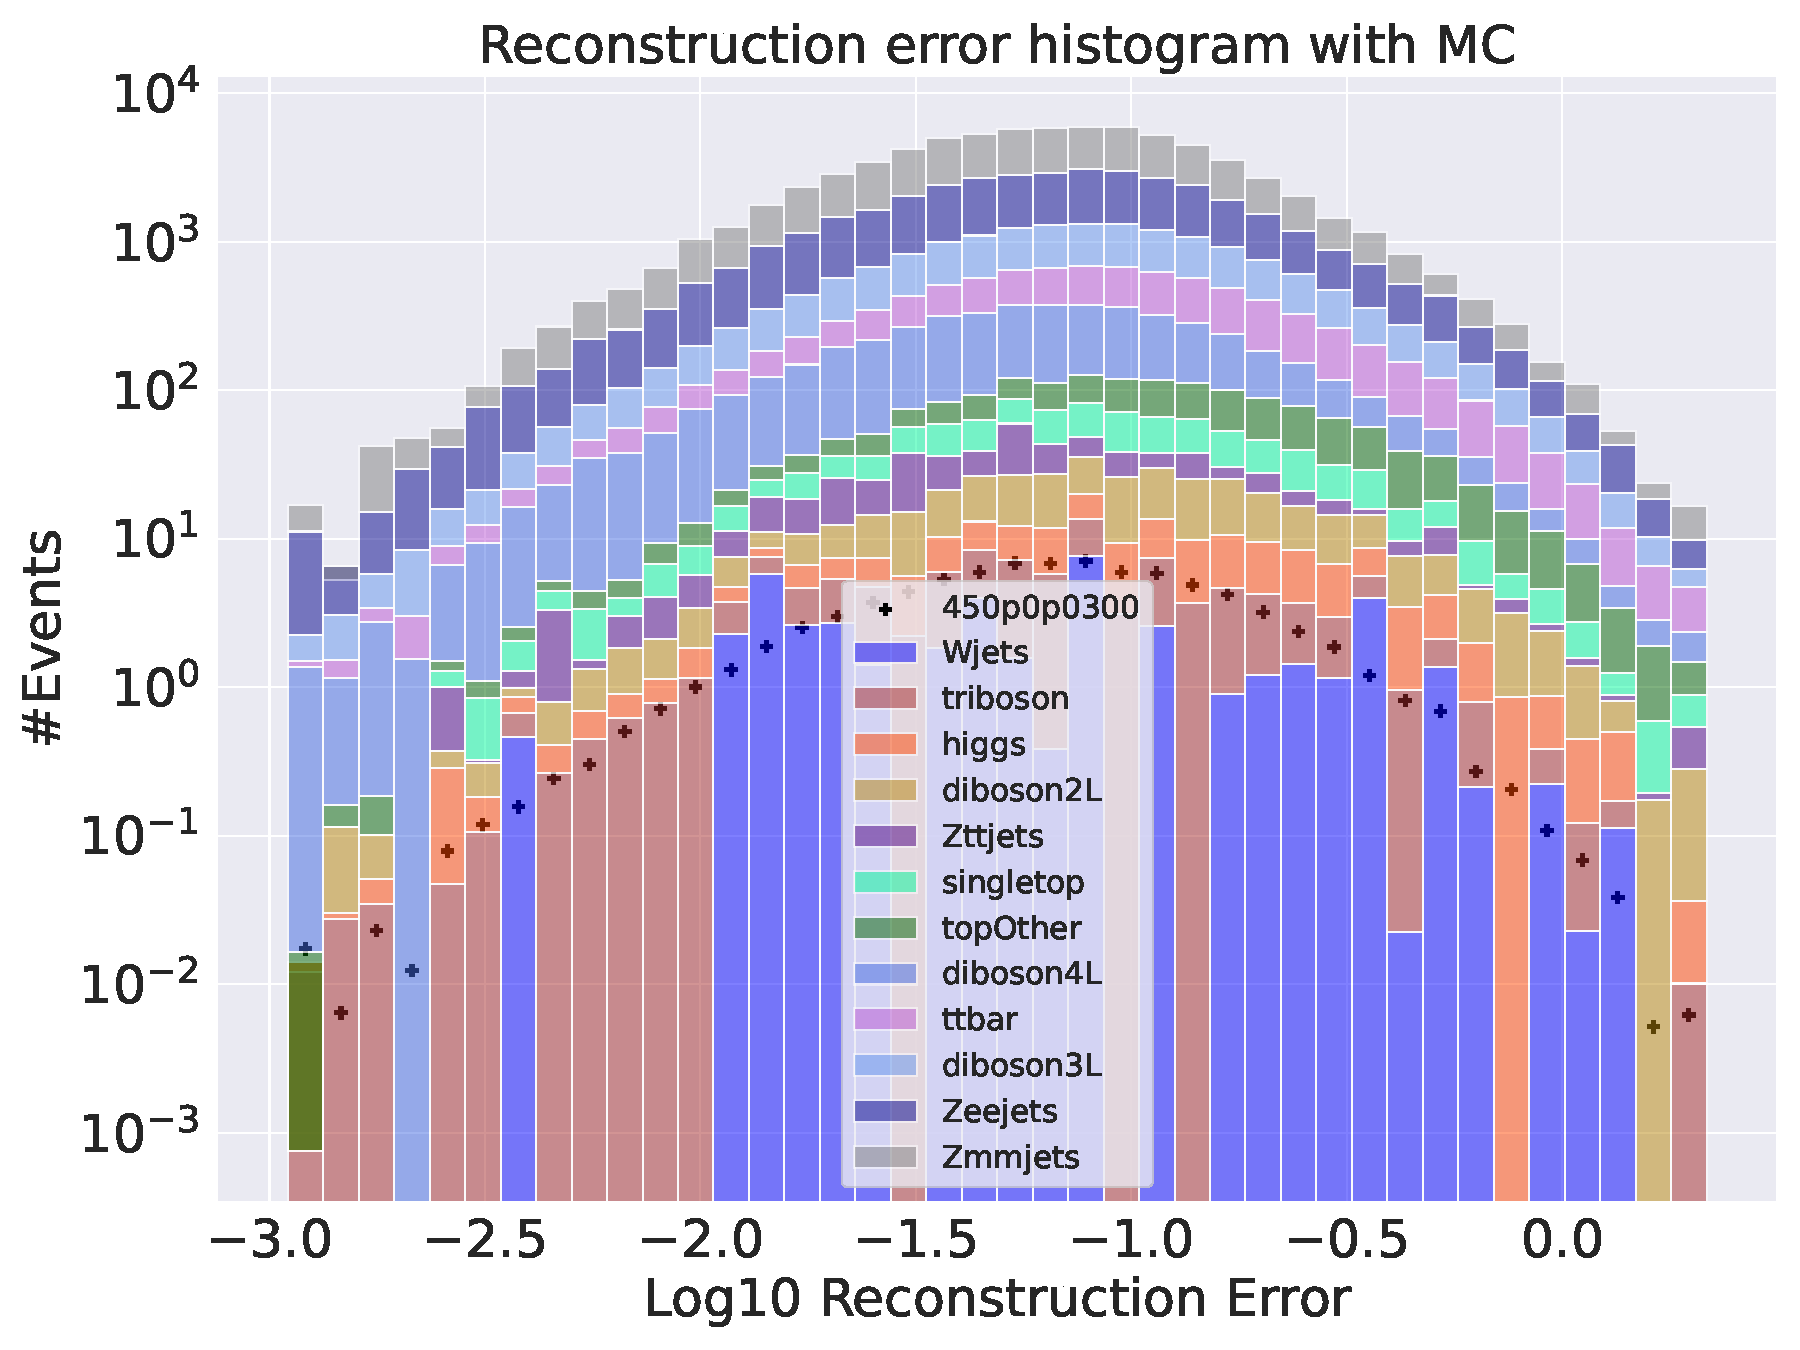
\includegraphics[width=\textwidth]{Figures/VAE_testing/big/3lep/b_data_recon_big_rm3_feats_sig_450p0p0300.pdf}
        \caption{ }
        \label{fig:VAE_3lep_big_450_3}
    \end{subfigure}
    \hfill
    \begin{subfigure}{.40\textwidth}
        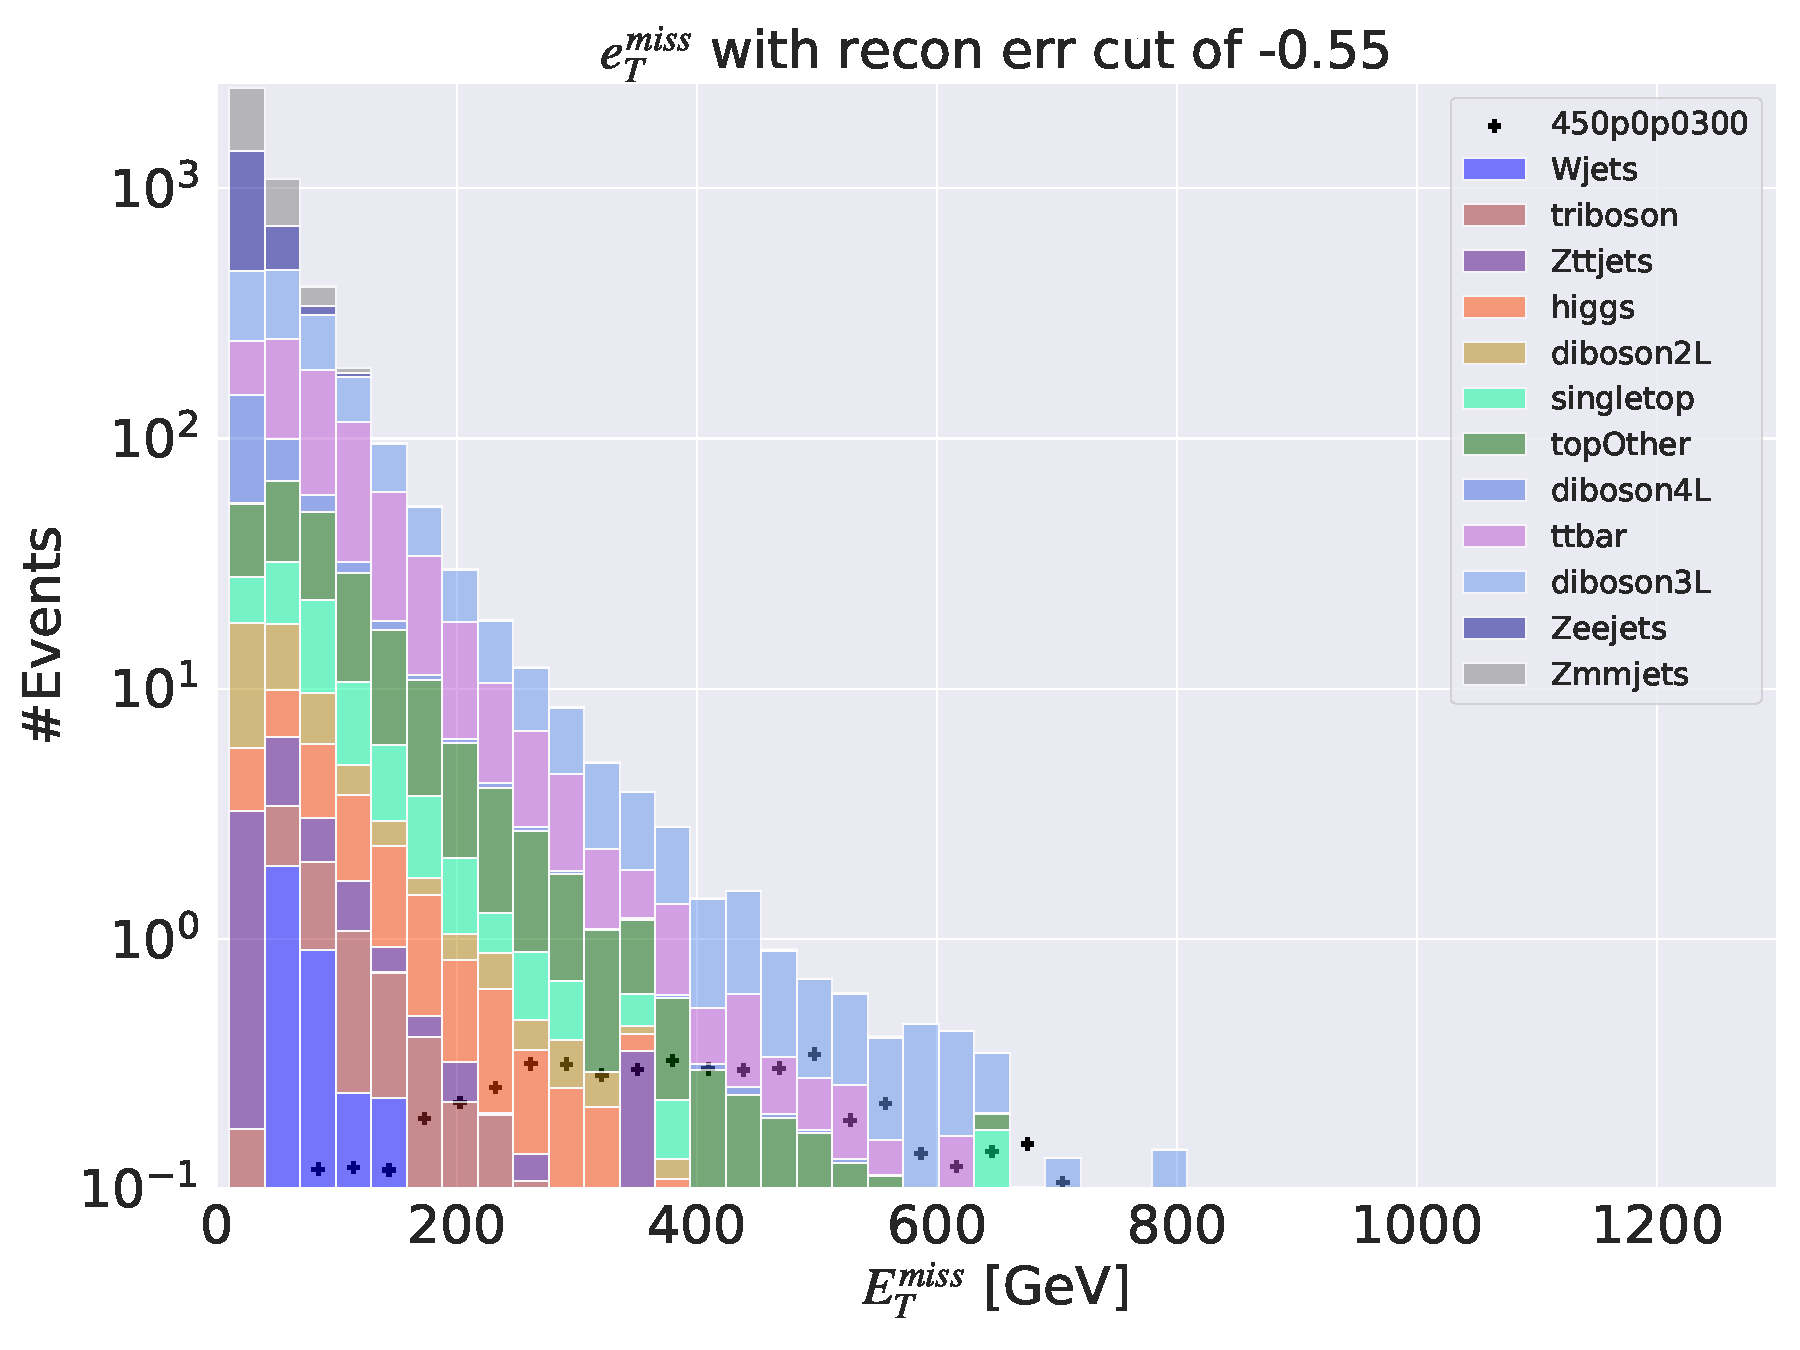
\includegraphics[width=\textwidth]{Figures/VAE_testing/big/3lep/b_data_recon_big_rm3_feats_sig_450p0p0300_etmiss_recon_errcut_-0.55.pdf}
        \caption{}
        \label{fig:VAE_3lep_big_etmiss_450_3}
    \end{subfigure}
    \hfill
    \begin{subfigure}{.40\textwidth}
        \includegraphics[width=\textwidth]{Figures/VAE_testing/big/3lep/b_data_recon_big_rm3_feats_sig_450p0p0300_mlll_recon_errcut_-0.55.pdf}
        \caption{}
        \label{fig:VAE_3lep_big_mlll_450_3}
    \end{subfigure}
    \hfill   
    \begin{subfigure}{.40\textwidth}
        \includegraphics[width=\textwidth]{Figures/VAE_testing/big/3lep/significance_etmiss_450p0p0300_-0.5484574357785665.pdf}
        \caption{}
        \label{fig:VAE_3lep_big_signi_450_3}
    \end{subfigure}
    \hfill      
    \caption[3lep deep network | $450p300$ | VAE | 3]{Reconstruction error, $e_T^{miss}$ signal region, $m_{lll}$ signal region and significance as function of 
    $e_T^{miss}$ for the deep variational autoencoder. Here the SUSY $450p300$ model is used.
    Figure \ref{fig:VAE_3lep_big_450_3} shows the reconstruction error 
    distribution for the SM MC and the SUSY signal. Here the autoencoder produce a bell-shape for background and 
    signal with little destinction. The peaks of the two distributions are not separated in reconstruction error. Figure \ref{fig:VAE_3lep_big_etmiss_450_3} 
    shows the $e_T^{miss}$ distribution for the SM MC and the SUSY signal in the signal region. 
    The signal region is made using a cut around $10^{-0.55}$. Some background is removed, and the peaks of the SM MC and signal 
    distributions are separated. Figure \ref{fig:VAE_3lep_big_mlll_450_3} shows the $m_{lll}$ distribution for the SM MC and the SUSY signal. 
    The shape of both distributions are displaying almost the same shape. Figure \ref{fig:VAE_3lep_big_signi_450_3} shows the significance as 
    function of $e_T^{miss}$. The peak is put around a cut of about 400 GeV in the $e_T^{miss}$, with a significance of around $0.94$.}
    \label{fig:VAE_3lep_big_rec_sig_signi_450_3}
\end{figure}

\begin{figure}[H]
    \centering
    \begin{subfigure}{.40\textwidth}
        \includegraphics[width=\textwidth]{Figures/VAE_testing/small/3lep/b_data_recon_big_rm3_feats_sig_450p0p0300.pdf}
        \caption{ }
        \label{fig:VAE_3lep_small_450_3}
    \end{subfigure}
    \hfill
    \begin{subfigure}{.40\textwidth}
        \includegraphics[width=\textwidth]{Figures/VAE_testing/small/3lep/b_data_recon_big_rm3_feats_sig_450p0p0300_etmiss_recon_errcut_-0.53.pdf}
        \caption{}
        \label{fig:VAE_3lep_small_etmiss_450_3}
    \end{subfigure}
    \hfill
    \begin{subfigure}{.40\textwidth}
        \includegraphics[width=\textwidth]{Figures/VAE_testing/small/3lep/b_data_recon_big_rm3_feats_sig_450p0p0300_mlll_recon_errcut_-0.53.pdf}
        \caption{}
        \label{fig:VAE_3lep_small_mlll_450_3}
    \end{subfigure}
    \hfill   
    \begin{subfigure}{.40\textwidth}
        \includegraphics[width=\textwidth]{Figures/VAE_testing/small/3lep/significance_etmiss_450p0p0300_-0.530518613616577.pdf}
        \caption{}
        \label{fig:VAE_3lep_small_signi_450_3}
    \end{subfigure}
    \hfill      
    \caption[3lep shallow network | $450p300$ | VAE | 3]{Reconstruction error, $e_T^{miss}$ signal region, $m_{lll}$ signal region and significance as function of 
    $e_T^{miss}$ for the shallow variational autoencoder. Here the SUSY $450p300$ model is used. 
    Figure \ref{fig:VAE_3lep_small_450_3} shows the reconstruction error 
    distribution for the SM MC and the SUSY signal. Here the autoencoder produce a bell-shape for background and 
    signal with little destinction. The peaks of the two distributions are not separated in reconstruction error. Figure \ref{fig:VAE_3lep_small_etmiss_450_3} 
    shows the $e_T^{miss}$ distribution for the SM MC and the SUSY signal in the signal region. 
    The signal region is made using a cut around $10^{-0.53}$. Some background is removed, and the peaks of the SM MC and signal 
    distributions are separated. Figure \ref{fig:VAE_3lep_small_mlll_450_3} shows the $m_{lll}$ distribution for the SM MC and the SUSY signal. 
    The shape of both distributions are displaying almost the same shape. Figure \ref{fig:VAE_3lep_small_signi_450_3} shows the significance as 
    function of $e_T^{miss}$. The peak is put around a cut of about 450 GeV in the $e_T^{miss}$, with a significance of around $0.81$.}
    \label{fig:VAE_3lep_small_rec_sig_signi_450_3}
\end{figure}








\begin{figure}[H]
    \centering
    \begin{subfigure}{.40\textwidth}
        \includegraphics[width=\textwidth]{Figures/VAE_testing/big/3lep/b_data_recon_big_rm3_feats_sig_800p0p050p.pdf}
        \caption{ }
        \label{fig:VAE_3lep_big_800_3}
    \end{subfigure}
    \hfill
    \begin{subfigure}{.40\textwidth}
        \includegraphics[width=\textwidth]{Figures/VAE_testing/big/3lep/b_data_recon_big_rm3_feats_sig_800p0p050p_etmiss_recon_errcut_-0.53.pdf}
        \caption{}
        \label{fig:VAE_3lep_big_etmiss_800_3}
    \end{subfigure}
    \hfill
    \begin{subfigure}{.40\textwidth}
        \includegraphics[width=\textwidth]{Figures/VAE_testing/big/3lep/b_data_recon_big_rm3_feats_sig_800p0p050p_mlll_recon_errcut_-0.53.pdf}
        \caption{}
        \label{fig:VAE_3lep_big_mlll_800_3}
    \end{subfigure}
    \hfill   
    \begin{subfigure}{.40\textwidth}
        \includegraphics[width=\textwidth]{Figures/VAE_testing/big/3lep/significance_etmiss_800p0p050p_-0.529426176908041.pdf}
        \caption{}
        \label{fig:VAE_3lep_big_signi_800_3}
    \end{subfigure}
    \hfill      
    \caption[3lep deep network | $800p50$ | VAE | 3]{Reconstruction error, $e_T^{miss}$ signal region, $m_{lll}$ signal region and significance as function of 
    $e_T^{miss}$ for the deep variational autoencoder. Here the SUSY $450p300$ model is used. 
    Figure \ref{fig:VAE_3lep_big_800_3} shows the reconstruction error 
    distribution for the SM MC and the SUSY signal. Here the autoencoder produce a bell-shape for background and 
    signal with little destinction. The peaks of the two distributions are not separated in reconstruction error. Figure \ref{fig:VAE_3lep_big_etmiss_800_3} 
    shows the $e_T^{miss}$ distribution for the SM MC and the SUSY signal in the signal region. 
    The signal region is made using a cut around $10^{-0.53}$. Some background is removed, and the peaks of the SM MC and signal 
    distributions are separated. Figure \ref{fig:VAE_3lep_big_mlll_800_3} shows the $m_{lll}$ distribution for the SM MC and the SUSY signal. 
    The shape of both distributions are displaying almost the same shape. Figure \ref{fig:VAE_3lep_big_signi_800_3} shows the significance as 
    function of $e_T^{miss}$. The peak is put around a cut of about 480 GeV in the $e_T^{miss}$, with a significance of around $0.21$.}
    \label{fig:VAE_3lep_big_rec_sig_signi_800_3}
\end{figure}

\begin{figure}[H]
    \centering
    \begin{subfigure}{.40\textwidth}
        \includegraphics[width=\textwidth]{Figures/VAE_testing/small/3lep/b_data_recon_big_rm3_feats_sig_800p0p050p.pdf}
        \caption{ }
        \label{fig:VAE_3lep_small_800_3}
    \end{subfigure}
    \hfill
    \begin{subfigure}{.40\textwidth}
        \includegraphics[width=\textwidth]{Figures/VAE_testing/small/3lep/b_data_recon_big_rm3_feats_sig_800p0p050p_etmiss_recon_errcut_-0.46.pdf}
        \caption{}
        \label{fig:VAE_3lep_small_etmiss_800_3}
    \end{subfigure}
    \hfill
    \begin{subfigure}{.40\textwidth}
        \includegraphics[width=\textwidth]{Figures/VAE_testing/small/3lep/b_data_recon_big_rm3_feats_sig_800p0p050p_mlll_recon_errcut_-0.46.pdf}
        \caption{}
        \label{fig:VAE_3lep_small_mlll_800_3}
    \end{subfigure}
    \hfill   
    \begin{subfigure}{.40\textwidth}
        \includegraphics[width=\textwidth]{Figures/VAE_testing/small/3lep/significance_etmiss_800p0p050p_-0.4571280959445052.pdf}
        \caption{}
        \label{fig:VAE_3lep_small_signi_800_3}
    \end{subfigure}
    \hfill      
    \caption[3lep shallow network | $800p50$ | VAE | 3]{Reconstruction error, $e_T^{miss}$ signal region, $m_{lll}$ signal region and significance as function of 
    $e_T^{miss}$ for the shallow variational autoencoder. Here the SUSY $450p300$ model is used. 
    Figure \ref{fig:VAE_3lep_small_800_3} shows the reconstruction error 
    distribution for the SM MC and the SUSY signal. Here the autoencoder produce a bell-shape for background and 
    signal with little destinction. The peaks of the two distributions are not separated in reconstruction error. Figure \ref{fig:VAE_3lep_small_etmiss_800_3} 
    shows the $e_T^{miss}$ distribution for the SM MC and the SUSY signal in the signal region. 
    The signal region is made using a cut around $10^{-0.46}$. Some background is removed, and the peaks of the SM MC and signal 
    distributions are separated. Figure \ref{fig:VAE_3lep_small_mlll_800_3} shows the $m_{lll}$ distribution for the SM MC and the SUSY signal. 
    The shape of both distributions are displaying almost the same shape. Figure \ref{fig:VAE_3lep_small_signi_800_3} shows the significance as 
    function of $e_T^{miss}$. The peak is put around a cut of about 480 GeV in the $e_T^{miss}$, with a significance of around $0.11$.}
    \label{fig:VAE_3lep_small_rec_sig_signi_800_3}
\end{figure}

